\documentclass[12pt,a4paper]{article}

\usepackage[T1]{fontenc}
\usepackage{lmodern}
%\usepackage{newtxtext}
\usepackage[scaled=.95]{newpxtext}
\usepackage{textcomp}
\usepackage{amsfonts}
\usepackage{amssymb}
\usepackage{mathtools}
\usepackage{bm}
\usepackage[all]{xy}
\usepackage{microtype}
\usepackage[svgnames]{xcolor}
\usepackage[margin=2.5cm]{geometry}
\usepackage{sectsty}
\allsectionsfont{\sffamily\color{Red}}
\paragraphfont{\sffamily}
\subparagraphfont{\sffamily}
\usepackage[font={sf,small},labelfont={bf,color=Red},labelsep=quad]{caption}
\usepackage{graphicx}
\graphicspath{{./fig/}}
\usepackage{booktabs}
\usepackage{enumitem}
\usepackage{natbib}
\usepackage{hyperxmp}
\usepackage[
bookmarks=true,bookmarksopen=true,
backref=page,colorlinks,allcolors=MidnightBlue,
]{hyperref}

\linespread{1.05}

%\renewcommand{\familydefault}{\sfdefault}

\newcommand{\email}[1]{\href{mailto:#1}{\texttt{#1}}}
\newcommand{\twitter}[1]{\href{https://twitter.com/#1}{\texttt{@#1}}}

\newcommand{\www}{\colorbox{MediumBlue}{\textcolor{White}{\textbf{\textsf{www}}}}}

\newcommand{\Section}[1]{%
\section*{#1}
\addcontentsline{toc}{section}{#1}}

\newcommand{\Subsection}[1]{%
\subsection*{#1}
\addcontentsline{toc}{subsection}{#1}}

\newcommand{\erratum}[1]{%
\subsubsection*{#1}
\addcontentsline{toc}{subsection}{#1}}

% TODO:
% Split lengthy paragraphs into shorter ones and use paragraph headers where appropriate to help
% the reader better understand the organization of the text.
\newcommand{\parhead}[1]{%
\paragraph{#1}
\addcontentsline{toc}{subsubsection}{#1}}

\title{More PRML Errata}
\author{Yousuke Takada \\ \email{yousuketakada@gmail.com}}
\date{\today}

\hypersetup{
pdftitle = {More PRML Errata},
pdfauthor = {Yousuke Takada},
pdfsubject = {Some more errata and additional comments for PRML},
pdfkeywords = {PRML, errata, Bishop, machine learning},
}

\begin{document}
\maketitle

\Section{Preface}
This report is an unofficial list of errata for \emph{Pattern Recognition and Machine Learning} or
PRML by \citet*{Bishop:PRML}.
In this report, I have compiled only errata
that are not (yet) listed in the official errata document~\citep{Svensen:PRML_errata}
at the time of this writing.
Currently, there are three versions of the official errata document,
corresponding to the first (2006), second (2007), and third (2009) printings of PRML;
consult the
\href{https://www.microsoft.com/en-us/research/people/cmbishop/\#prml-book}{support page}
for how to identify which printing your copy of PRML is from.\footnote{%
The last line but one of the bibliographic information page
(the page immediately preceding the dedication page) of my copy of PRML
reads ``9 8 7 (corrected at 6th printing 2007).''
Note that, although it says it is from the ``6th printing,''
it is actually from the \emph{second} printing according to
the official errata document~\citep{Svensen:PRML_errata}
so that I refer to Version~2 of the official errata.}

I have tried to follow the terminology and the notation used in PRML and the official errata
as closely as possible.
In particular, when specifying the location of an error,
I follow the notational conventions (such as ``Paragraph~2, Line~\textminus1'')
adopted by \citet{Svensen:PRML_errata}.
As the official errata document ``is intended to be complete,''
this report also tries to correct even trivial typographical errors as well.

PRML is arguably such a great textbook in the field of machine learning
that it is extremely helpful and easier to understand than any other similar account.
That said, there are a few subtleties
that some readers might have hard time to appreciate.
In hopes to help such readers get out of struggle or
obtain a better grasp on some important concepts,
I have also included in this report some comments and suggestions for improving the readability
to which I would have liked to refer when I first read PRML.

It should be noted that the readers of the Japanese edition of PRML will find its
\href{http://ibisforest.org/index.php?PRML}{support page} (in Japanese) useful.
Along with other information such as the contents,
it lists errata specific to the Japanese edition as well as
some additional errata for the English edition,
which have also been included in this report for the reader's convenience.

I welcome all comments and suggestions regarding this report;
please send me any such feedback via email or, preferably,
by creating an ``issue'' or a ``pull request'' at the following GitHub repository
\begin{center}
\url{https://github.com/yousuketakada/prml\_errata}
\end{center}
where you can find the source code of this report
as well as other supporting material.

\Subsection{Acknowledgements}
I would like to thank those who have informed me of yet more errata and clarifications
incorporated in this report.
In particular, I am grateful to
Christopher Sahnwaldt and
Mark-Jan Nederhof
for their helpful comments and discussions.

\Section{Corrections and Comments}

\erratum{Page~xi}
% See https://github.com/yousuketakada/prml_errata/pull/1
Paragraph~\textminus2, Line~1:
$\left|f(x)/g(x)\right|$ should read $\left|g(x)/f(x)\right|$ (with the functions swapped).
Moreover, the limit we take is \emph{not} necessarily the one specified in the text,
i.e., $x \to \infty$,
but is often implied by the context as follows.

\parhead{Big O notation}
The big O notation~$g(x) = O\left(f(x)\right)$ generally denotes that
$\left|g(x)/f(x)\right|$ is bounded as $x \to c$
where, if $c$ is not given explicitly,
$c = 0$ for a Taylor series such as (2.299) or (D.1); or
$c = \infty$ for an asymptotic series such as (10.241) or
for computational complexity (see, e.g., Section~5.2.3),
for example.
See \citet{NIST:DLMF} for other asymptotic and order notations.

\erratum{Page~5}
Equation~(1.1):
The lower ellipsis ($\ldots$) should be centered ($\cdots$).\footnote{%
The \LaTeX{} command~\texttt{\char`\\cdots} or,
with the \texttt{amsmath} or \texttt{mathtools} package,
\texttt{\char`\\dots} (in most cases) will do.}
Specifically, (1.1) should read
\begin{equation}
y(x, \mathbf{w}) = w_0 + w_1 x + w_2 x^2 + \dots + w_M x^M = \sum_{j=0}^{M} w_j x^j .
\end{equation}

\erratum{Page~10}
The text after (1.4):
The lower ellipsis ($\ldots$) should be centered ($\cdots$).

\erratum{Page~18}
Equation~(1.27):
It should be noted that
the transformation~$g : \mathcal{Y} \to \mathcal{X}$ must be \emph{bijective} or, equivalently,
\emph{invertible} in order for the change of variables~(1.27) to be meaningful
where $\mathcal{X}$ and $\mathcal{Y}$ are the domains of
the distributions~$p_x(\cdot)$ and $p_y(\cdot)$, respectively.\footnote{%
A function~$f : \mathcal{X} \to \mathcal{Y}$ is said to be \emph{bijective}
(or \emph{one-to-one correspondence})
if, for any $y \in \mathcal{Y}$, there exists a unique $x \in \mathcal{X}$ such that $y = f(x)$.
Note also that bijectivity is equivalent to invertibility:
A function~$f : \mathcal{X} \to \mathcal{Y}$ is bijective if and only if $f$ is \emph{invertible},
i.e., there exists an inverse function~$f^{-1} : \mathcal{Y} \to \mathcal{X}$
(which is, of course, also bijective)
such that $f^{-1} \circ f$ is the identity function on $\mathcal{X}$,
meaning that $x = f^{-1}(f(x))$ for any $x \in \mathcal{X}$.}
This can be easily understood by noting that, if we have
\begin{align}
\int_{\mathcal{X}_0} p_x(x) \, \mathrm{d}x &=
\int_{\mathcal{Y}_0} p_x(x)
\left| \frac{\mathrm{d}x}{\mathrm{d}y} \right| \mathrm{d}y
\\
&=
\int_{\mathcal{Y}_0} p_x(g(y))
\left| g'(y) \right| \mathrm{d}y
\end{align}
for any pair of $\mathcal{X}_0 \subset \mathcal{X}$ and $\mathcal{Y}_0 \subset \mathcal{Y}$
such that $\mathcal{X}_0 = g(\mathcal{Y}_0)$ or $\mathcal{Y}_0 = g^{-1}(\mathcal{X}_0)$,\footnote{%
Let $f : \mathcal{X} \to \mathcal{Y}$ be
some function from the set~$\mathcal{X}$ to the set~$\mathcal{Y}$.
The image of a subset~$\mathcal{X}_0 \subset \mathcal{X}$ under $f$ is denoted by
$f(\mathcal{X}_0) \subset \mathcal{Y}$.}
then we can identify the integrand of the right hand side as $p_y(y)$.

\parhead{Multivariate change of variables}
Similarly, the multivariate version of the change of variables formula is given by
\begin{equation}
p(\mathbf{y}) =
p(\mathbf{x})
\left|
\operatorname{det}\left(\frac{\partial\mathbf{x}}{\partial\mathbf{y}}\right)
\right|
\label{eq:multivariate_change_of_variables}
\end{equation}
where the transformation between $\mathbf{x}$ and $\mathbf{y}$ is again assumed to be bijective.

\erratum{Page~42}
% Due to Mark-Jan Nederhof
Paragraph~1, Line~1:
``the class~$j$'' should read ``class~$\mathcal{C}_j$.''

\erratum{Page~44}
% Due to Mark-Jan Nederhof
Paragraph~2, Line~\textminus3:
Insert a space before the sentence starting ``There has been\dots''
(\emph{the third printing only}).\footnote{%
Something strange must have happened in the third (2009) printing,
leading to some spacing issues where a sentence ends with a reference number
such as ``Figure~1.27.''
We can also find other ``regression'' errors in the third printing.
Such errors are marked ``\emph{the third printing only}'' in this report.}

\erratum{Page~46}
Equation~(1.85):
A period (.) should terminate (1.85).

\erratum{Page~47}
Paragraph~1, Line~\textminus1:
$\mathbb{E}_{t}\left[\mathbf{t}\middle|\mathbf{x}\right]$
should read
$\mathbb{E}_{\mathbf{t}}\left[\mathbf{t}\middle|\mathbf{x}\right]$
(the subscript should be the vector~$\mathbf{t}$).

\erratum{Page~47}
Equation~(1.90):
The quantity~$\operatorname{var}\left[ t \middle| \mathbf{x} \right]$ is
a \emph{conditional variance},
which is defined similarly to the \emph{conditional expectation}~(1.37) so that
\begin{equation}
\operatorname{var}\left[ t \middle| \mathbf{x} \right] =
\mathbb{E}\left[
\left( t - \mathbb{E}\left[t\middle|\mathbf{x}\right] \right)^2 \middle| \mathbf{x}
\right]
\end{equation}
where we have omitted the subscript~$t$ in what should be
$\mathbb{E}_{t}\left[\cdot\middle|\mathbf{x}\right]$

\erratum{Page~51}
Equation~(1.98):
Following the notation~(1.93) for \emph{entropy},
we should write the left hand side of (1.98) as
$\operatorname{H}[X]$ instead of $\operatorname{H}[p]$ so that
\begin{equation}
\operatorname{H}[X] = - \sum_{i} p(x_{i}) \ln p(x_{i}) .
\label{eq:entropy_in_nats}
\end{equation}
As suggested in the first paragraph of Appendix~D on Page~703,
if we regard the (differential) entropy~$\operatorname{H}[\cdot]$ as a \emph{functional},
then we see that
``the entropy could equally well have been written as $\operatorname{H}[p]$.''
However, it is probably better to maintain the notational consistency here.

\erratum{Page~56}
Equation~(1.116):
In general, we cannot interpret $\lambda_i$ in \emph{Jensen's inequality}~(1.115) as
the probability distribution over a discrete random variable~$x$
such that $\lambda_i \equiv p(x = x_i)$
because, since (1.115) holds for any $\left\{x_i\right\}$,
we can take, say, $x_i = x_j$ and $\lambda_i \neq \lambda_j$ where $i \neq j$,
assigning different probabilities for the same value of $x$.
Actually, (1.116) is a special case of (1.115).
An equivalent of (1.115) in terms of random variables can be derived as follows.

\parhead{Jensen's inequality in terms of random variables}
In order to interpret (1.115) probabilistically,
we instead introduce another set of underlying random variables~$\mathbf{z}$
such that $\lambda_i \equiv p(\mathbf{z} = \mathbf{z}_i)$ and
a function~$\xi(\cdot)$ such that $x_i \equiv \xi(\mathbf{z}_i)$,
giving a result slightly more general than (1.116)
\begin{equation}
f\left(\mathbb{E}_{\mathbf{z}}\left[\xi(\mathbf{z})\right]\right)
\leqslant \mathbb{E}_{\mathbf{z}}\left[f\left(\xi(\mathbf{z})\right)\right]
\label{eq:Jensen_inequality_expectation_with_z}
\end{equation}
where $f(\cdot)$ is a convex function but $\xi(\cdot)$ can be any.
Moreover, if $f(\cdot)$ is strictly convex,
the equality in \eqref{eq:Jensen_inequality_expectation_with_z} holds if and only if
$\xi(\cdot)$ is \emph{essentially constant},
meaning that there exists some constant~$\xi_0$ and
$\xi(\mathbf{z}) = \xi_0$ for almost\footnote{%
Here, the term~``almost'' means that there may be some exceptions
but they can occur only with probability zero so that we can safely ignore them;
it is formally defined in a branch of mathematics called \emph{measure theory},
which however ``lies outside the scope of [PRML]'' (Page~19, Paragraph~3, Line~\textminus5).
As in PRML, we omit the term~``almost'' for brevity in the rest of this report.}
all $\mathbf{z}$ such that $p(\mathbf{z}) > 0$
(in other words, if we regard $\xi = \xi(\mathbf{z})$ as a random variable,
we have $\xi = \xi_0$ almost surely, i.e., with probability one),
in which case we have $\mathbb{E}_{\mathbf{z}}\left[\xi(\mathbf{z})\right] = \xi_0$
and the both sides of \eqref{eq:Jensen_inequality_expectation_with_z} equal $f(\xi_0)$.
See Figure~\ref{fig:Jensen_inequality} for an intuitive, physical ``proof'' of
the inequality~\eqref{eq:Jensen_inequality_expectation_with_z}.

\begin{figure}
\centering
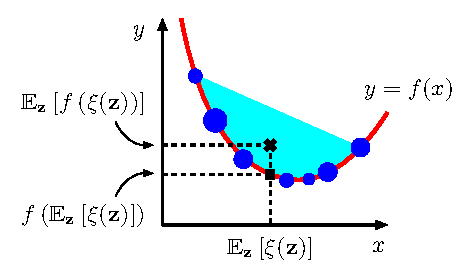
\includegraphics{jensen_inequality.eps}
\caption{A physical ``proof'' of
Jensen's inequality~\citep{MacKay:Information}.
Let us suppose that we have a set of point masses~$m_i = p(\mathbf{z}=\mathbf{z}_i)$,
denoted by filled blue circles ({\large\textcolor{blue}{$\bullet$}})
with areas proportional to $m_i$,
and place them at the corresponding
locations~$(x, y) = \left(\xi(\mathbf{z}_i), f(\xi(\mathbf{z}_i))\right)$
on a convex curve~$y = f(x)$.
The center of gravity of those masses, which is $\left(
\mathbb{E}_{\mathbf{z}}\left[\xi(\mathbf{z})\right],
\mathbb{E}_{\mathbf{z}}\left[f\left(\xi(\mathbf{z})\right)\right]
\right)$, denoted by a cross sign ($\boldsymbol{\times}$),
must lie above the convex curve and thus right above the point~$\left(
\mathbb{E}_{\mathbf{z}}\left[\xi(\mathbf{z})\right],
f\left(\mathbb{E}_{\mathbf{z}}\left[\xi(\mathbf{z})\right]\right)
\right)$ on the curve, denoted by a filled square ($\blacksquare$),
showing Jensen's inequality~\eqref{eq:Jensen_inequality_expectation_with_z}.
One can also see that, if $f(\cdot)$ is strictly convex,
the equality in \eqref{eq:Jensen_inequality_expectation_with_z}
implies that $\xi(\cdot)$ is essentially constant
(it is trivial to show that the converse is true).}
\label{fig:Jensen_inequality}
\end{figure}

Since the random variables~$\mathbf{z}$ as well as their probability~$p(\mathbf{z})$ can be chosen
arbitrarily,
it makes sense to write $\mathbf{z}$ implicit in \eqref{eq:Jensen_inequality_expectation_with_z},
giving a simpler form of Jensen's inequality
\begin{equation}
f\left(\mathbb{E}\left[\xi\right]\right)
\leqslant \mathbb{E}\left[f\left(\xi\right)\right] .
\end{equation}
For continuous random variables, we have
\begin{equation}
f\left(\int\xi(\mathbf{x}) p(\mathbf{x}) \,\mathrm{d}\mathbf{x}\right) \leqslant
\int f\left(\xi(\mathbf{x})\right) p(\mathbf{x}) \,\mathrm{d}\mathbf{x}
\label{eq:Jensen_inequality_continuous}
\end{equation}
where we have used $\mathbf{x}$ to denote the underlying random variables
for which we take the expectations.
By making use of \eqref{eq:Jensen_inequality_continuous},
one can show that
the \emph{Kullback-Leibler divergence}~$\operatorname{KL}\left( p \middle\| q \right)$
given by (1.113) satisfies \emph{Gibbs's inequality}
\begin{equation}
\operatorname{KL}\left( p \middle\| q \right) \geqslant 0
\label{eq:Gibbs_inequality}
\end{equation}
with equality if and only if $p(\mathbf{x}) = q(\mathbf{x})$ almost everywhere.
See the following erratum for more details.

\erratum{Page~56}
Equation~(1.118):
There are some difficulties in the derivation~(1.118) of
Gibbs's inequality~\eqref{eq:Gibbs_inequality}.
First, the quantity~$\xi(\mathbf{x}) = q(\mathbf{x})/p(\mathbf{x})$ is undefined for $\mathbf{x}$
such that $p(\mathbf{x}) = 0$.
Second, the convex function~$f(\xi) = -\ln\xi$ is undefined for $\xi = 0$,
which occurs where $q(\mathbf{x}) = 0$ and $p(\mathbf{x}) > 0$.
In order to avoid these difficulties,
we should take a different approach~\citep{MacKay:Information,KullbackLeibler:Information}
in which we make use of Jensen's inequality~\eqref{eq:Jensen_inequality_continuous}
with respect to $q(\mathbf{x})$ where
we identify $f(\xi) = \xi\ln\xi$ and
$\xi(\mathbf{x}) = p(\mathbf{x})/q(\mathbf{x})$.
Note that we can safely proceed with this approach
because we can assume $q(\mathbf{x}) > 0$
without loss of generality as we shall see in the following.

\parhead{A proof of Gibbs's inequality}
Let us first examine the behavior of the integrand of
the Kullback-Leibler divergence~$\operatorname{KL}\left( p \middle\| q \right)$
\begin{equation}
p(\mathbf{x}) \ln p(\mathbf{x}) - p(\mathbf{x}) \ln q(\mathbf{x})
\label{eq:integrand_of_KL}
\end{equation}
where $q(\mathbf{x})$ or $p(\mathbf{x})$ vanishes.
We notice that, if $q(\mathbf{x}) \to 0$ for $\mathbf{x}$ such that $p(\mathbf{x}) > 0$,
the integrand~\eqref{eq:integrand_of_KL} diverges so that
$\operatorname{KL}\left( p \middle\| q \right) \to \infty$.
On the other hand, the integrand~\eqref{eq:integrand_of_KL} always vanishes for $\mathbf{x}$
such that $p(\mathbf{x}) = 0$ regardless of the values of $q(\mathbf{x})$.\footnote{%
Recall that we have defined $0 \log_2 0 \equiv 0$ or, equivalently, $0 \ln 0 \equiv 0$
(Page~49, Paragraph~2, Line~\textminus2) so that
the entropy in ``bits''~(1.93) or ``nats''~\eqref{eq:entropy_in_nats} is well-defined.}
Therefore, in order for $\operatorname{KL}\left( p \middle\| q \right)$ to be well-defined,
one must have $p(\mathbf{x}) = 0$ wherever $q(\mathbf{x}) = 0$;
this property is called \emph{zero-forcing} (see also Section~10.1.2).

Assuming the zero-forcing condition, that is,
$p(\mathbf{x}) = 0$ for all $\mathbf{x}$ such that $q(\mathbf{x}) = 0$,
we can consider the integration in $\operatorname{KL}\left( p \middle\| q \right)$
only over the \emph{support}~$\Omega = \{ \mathbf{x} \mid q(\mathbf{x}) > 0 \}$ of $q(\mathbf{x})$.
Identifying $f(\xi) = \xi\ln\xi$ (see Figure~\ref{fig:x_ln_x}) and
$\xi(\mathbf{x}) = p(\mathbf{x})/q(\mathbf{x})$,
we have
\begin{align}
\operatorname{KL}\left( p \middle\| q \right)
&= \int_{\Omega} q(\mathbf{x})
\frac{p(\mathbf{x})}{q(\mathbf{x})}
\ln \left\{\frac{p(\mathbf{x})}{q(\mathbf{x})}\right\}
\mathrm{d}\mathbf{x} \\
&= \int_{\Omega} q(\mathbf{x})
f\left(\xi(\mathbf{x})\right)
\mathrm{d}\mathbf{x} \\
&\geqslant f\left(
\int_{\Omega} q(\mathbf{x}) \xi(\mathbf{x}) \, \mathrm{d}\mathbf{x}
\right) \\
&= f\left(\int_{\Omega} p(\mathbf{x}) \, \mathrm{d}\mathbf{x} \right) \\
&= f(1) = 0
\end{align}
where we have used \eqref{eq:Jensen_inequality_continuous} with respect to $q(\mathbf{x})$
(instead of $p(\mathbf{x})$).
Note that, since $q(\mathbf{x}) > 0$ over $\Omega$, we see that
$\xi(\mathbf{x}) = p(\mathbf{x})/q(\mathbf{x}) \geqslant 0$ is well-defined over $\Omega$ and
so is $f\left(\xi(\mathbf{x})\right) = \xi(\mathbf{x})\ln\xi(\mathbf{x})$.
Since $f(\xi)$ is strictly convex,
the equality~$\operatorname{KL}\left( p \middle\| q \right) = 0$ holds if and only if
$\xi(\mathbf{x}) = p(\mathbf{x})/q(\mathbf{x})$ is constant over $\Omega$,
which, together with the zero-forcing condition, yields the equality condition that
$p(\mathbf{x}) = q(\mathbf{x})$ for all $\mathbf{x}$.

\begin{figure}
\centering
\input{fig/x_ln_x_plot.tex}
\caption{Plot of $f(x) = x \ln x$.
The function~$f(x)$ is a strictly convex function defined over $\left[0, \infty\right)$
where we have defined $f(0) = 0 \ln 0 \equiv 0$.
The curve~$y = f(x)$ takes the minimum at $(x, y) = \left(e^{-1}, -e^{-1}\right)$.
The roots (the values of $x$ such that $f(x) = 0$) are $x = 0$ and $x = 1$.}
\label{fig:x_ln_x}
\end{figure}

\erratum{Page~59}
% Due to Mark-Jan Nederhof
Exercise~1.7, Line~2:
``To do this consider, the\dots'' should be
``To do this, consider the\dots''

\erratum{Page~61}
% Due to Mark-Jan Nederhof
Exercise~1.15, Line~\textminus1:
Add a period (.) at the end of the last sentence.

\erratum{Page~62}
Exercise~1.18, the text after (1.142):
``Gamma'' should read ``gamma'' (without capitalization).

\erratum{Page~64}
% Due to Mark-Jan Nederhof
Exercise~1.28, Line~1:
In Section~1.6,
the quantity~$h(x)$ is introduced as a measure of the information gained on observing
the random variable~$x$,
whereas the \emph{entropy} is the average of $h(x)$ over $x$.
The first sentence should thus read, e.g.,
``In Section~1.6, we introduced the idea of entropy as
the average of the information~$h(x)$ gained\dots''

\erratum{Page~64}
% Due to Mark-Jan Nederhof
Exercise~1.28, Lines~3 and 4:
``the entropy functions are additive, so that\dots'' should read, e.g.,
``the information~$h(\cdot)$ is additive so that\dots''
(see also the previous erratum).

\erratum{Page~70}
Paragraph~\textminus1, Line~\textminus1:
The lower ellipsis ($\ldots$) should be centered ($\cdots$).

\erratum{Page~76}
Equations~(2.34) and (2.35):
The \emph{multinomial coefficient}~(2.35) is better written as
\begin{equation}
\binom{N}{m_1, m_2, \dots, m_K} \equiv
\frac{N!}{m_1 ! \, m_2 ! \cdots m_K !}
\label{eq:multinomial_coefficient}
\end{equation}
where $m_1, m_2, \dots, m_K$ are comma separated in the left hand side
so as not to be confused with a function of the product of $m_1, m_2, \dots, m_K$.
Also, the lower ellipsis ($\ldots$) in the right hand side of (2.35)
should be centered ($\cdots$) as shown in \eqref{eq:multinomial_coefficient}.

\erratum{Page~78}
The caption of Figure~2.5:
``$\left\{ \alpha_k \right\} = 0.1$'' should read ``$\alpha_k = 0.1$ for all $k$'' and so on.

\erratum{Page~80}
Equation~(2.52):
We usually take eigenvectors~$\mathbf{u}_{i}$ to be the columns of $\mathbf{U}$ as in (C.37).
If we follow this convention, (2.52) and the following text should read
\begin{equation}
\mathbf{y} = \mathbf{U}^{\operatorname{T}} (\mathbf{x} - \bm{\mu})
\label{eq:change_of_variable_x_to_y}
\end{equation}
where $\mathbf{U}$ is a matrix whose columns are given by $\mathbf{u}_{i}$ so that
$\mathbf{U} = \left( \mathbf{u}_{1}, \dots,  \mathbf{u}_{D}\right)$.
From (2.46) it follows that $\mathbf{U}$ is an \emph{orthogonal} matrix, i.e.,
it satisfies $\mathbf{U}^{\operatorname{T}}\mathbf{U} = \mathbf{I}$ and hence also
$\mathbf{U}\mathbf{U}^{\operatorname{T}} = \mathbf{I}$ where $\mathbf{I}$ is the identity matrix.

\erratum{Page~81}
Equations~(2.53) and (2.54):
If we write the change of variable from $\mathbf{x}$ to $\mathbf{y}$ as
\eqref{eq:change_of_variable_x_to_y} instead of (2.52),
the Jacobian matrix~$\mathbf{J} = \left( J_{ij} \right)$ is simply given by $\mathbf{U}$.
Equation~(2.53) should read
\begin{equation}
J_{ij} = \frac{\partial x_i}{\partial y_j} = U_{ij}
\end{equation}
where $U_{ij}$ is the $(ij)$-th element of $\mathbf{U}$.
The square of the determinant of the Jacobian matrix~(2.54) can then be evaluated as
\begin{equation}
\left| \mathbf{J} \right|^{2} = \left| \mathbf{U} \right|^{2}
= \left| \mathbf{U}^{\operatorname{T}} \right| \left| \mathbf{U} \right|
= \left| \mathbf{U}^{\operatorname{T}} \mathbf{U} \right|
= \left| \mathbf{I} \right| = 1.
\end{equation}

\erratum{Page~81}
The text after (2.54):
Since the Jacobian matrix~$\mathbf{J}$ is only assumed to be orthogonal here,
the determinant of $\mathbf{J}$ can be either positive or negative so that
we should write $\left| \mathbf{J} \right| = \pm 1$
instead of $\left| \mathbf{J} \right| = 1$.

\erratum{Page~82}
Equation~(2.56):
We should take the absolute value of the determinant for the same reason given above so that
the factor~$\left| \mathbf{J} \right|$ should read
$\left| \operatorname{det}\left( \mathbf{J} \right) \right|$.
Note however that it is not recommended to write $\left|\left| \mathbf{J} \right|\right|$ to mean
$\left| \operatorname{det}\left( \mathbf{J} \right) \right|$
because $\left|\left| \mathbf{J} \right|\right|$ is confusingly similar to
the \emph{matrix norm}~$\left\| \mathbf{J} \right\|$,
which usually refers to the largest singular value of $\mathbf{J}$~\citep{GvL:MC}.
This notational inconsistency is caused by the abuse of the notation~$|\cdot|$ for
both the absolute value and the matrix determinant;
if we always use $\operatorname{det}(\cdot)$ for the determinant, confusion will not arise
and the notation be consistent.

\parhead{Notation for absolute determinant}
An alternative solution to the problem of notational inconsistency mentioned above would be
to explicitly define $\left| \mathbf{A} \right|$ as the absolute value of the determinant of
a square matrix~$\mathbf{A}$, i.e.,
\begin{equation}
\left| \mathbf{A} \right| \equiv \left| \operatorname{det}\left( \mathbf{A} \right) \right|
\label{eq:abs_of_matrix_determinant}
\end{equation}
so that we have $\left|\mathbf{J}\right| = 1$ and (2.56) holds as is.
Note also that this notation~\eqref{eq:abs_of_matrix_determinant} is mostly consistent
in other part of PRML because we have
$\left| \mathbf{A} \right| = \operatorname{det}\left( \mathbf{A} \right)$
for any positive-semidefinite matrix~$\mathbf{A} \succeq 0$ (see Appendix~C) and
most matrices for which we take determinants are in fact positive definite.\footnote{%
In this report, we assume as customary that
the concept of positive/negative (semi)definiteness is restricted to symmetric matrices.
For example, when we say ``$\mathbf{A}$ is positive definite'' or $\mathbf{A} \succ 0$,
we implicitly assume that $\mathbf{A}$ is also symmetric so that
$\mathbf{A}^{\operatorname{T}} = \mathbf{A}$,
though we still sometimes say ``$\mathbf{A}$ is symmetric positive definite'' to avoid confusion.}
Such positive-definite matrices include
the covariance~$\bm{\Sigma}$ or the precision~$\bm{\Lambda}$ of
the multivariate Gaussian distribution and
the scale matrix~$\mathbf{W}$ of the Wishart distribution (see Appendix~B).

\erratum{Page~82}
Two lines above (2.59):
``the term in $\mathbf{z}$ in the factor~$(\mathbf{z} + \bm{\mu})$''
should read
``the term~$\mathbf{z}$ in the factor~$(\mathbf{z} + \bm{\mu})$''
(Remove the first occurrence of ``in'').

\erratum{Page~90}
Paragraph~\textminus1, Line~2:
The partitioned vector should read
$\mathbf{x} = \left(
\mathbf{x}_a^{\operatorname{T}}, \mathbf{x}_b^{\operatorname{T}}
\right)^{\operatorname{T}}$.

\erratum{Page~91}
% Due to Mark-Jan Nederhof
Paragraph~1, Line~1:
``linear Gaussian'' should read ``linear-Gaussian'' (with hyphenation)
for consistency with other part of PRML (see, e.g., Section~8.1.4).

\erratum{Page~93}
Equation~(2.120):
The vector derivative operator~$\frac{\partial}{\partial \bm{\mu}}$ should read
the \emph{gradient}~$\nabla_{\bm{\mu}}$
if we use the notation~\eqref{eq:gradient_of_vector_wrt_vector} we adopt in this report.

\erratum{Pages~93 and 94}
Equations~(2.121) and (2.122):
We obtain the maximum likelihood solutions~$\bm{\mu}_\text{ML}$ and $\bm{\Sigma}_\text{ML}$
for the Gaussian by setting the derivatives of
the log likelihood function~$\ln p\left(\mathbf{X}\middle| \bm{\mu}, \bm{\Sigma}\right)$
given by (2.118) with respect to $\bm{\mu}$ and $\bm{\Sigma}$ equal to zero,
which, however, only implies that $\bm{\mu}_\text{ML}$ and $\bm{\Sigma}_\text{ML}$ are
stationary points.
We should also show that
$\bm{\mu}_\text{ML}$ and $\bm{\Sigma}_\text{ML}$ indeed maximize the likelihood
as discussed in the following.

\parhead{Maximum likelihood for Gaussian}
Let us first maximize the likelihood function with respect to the mean~$\bm{\mu}$.
This can be easily done by noting that
the log likelihood~(2.118) is quadratic in $\bm{\mu}$ so that
\begin{equation}
\ln p\left(\mathbf{X}\middle| \bm{\mu}, \bm{\Sigma}\right) =
-\frac{N}{2}
\left(\bm{\mu} - \bm{\mu}_{\text{ML}}\right)^{\operatorname{T}} \bm{\Sigma}^{-1}
\left(\bm{\mu} - \bm{\mu}_{\text{ML}}\right)
+ \text{const}
\label{eq:log_likelihood_wrt_mu}
\end{equation}
where $\bm{\mu}_{\text{ML}}$ is given by (2.121)
and the terms independent of $\bm{\mu}$ have been absorbed into ``$\text{const}$.''
Since the covariance~$\bm{\Sigma}$ is positive definite and so is its inverse~$\bm{\Sigma}^{-1}$,
we see that the log likelihood~\eqref{eq:log_likelihood_wrt_mu} is concave
with respect to $\bm{\mu}$ and
that $\bm{\mu}_\text{ML}$ indeed maximizes the likelihood.

Next, we consider maximization with respect to the covariance~$\bm{\Sigma}$.
The maximum likelihood solution~$\bm{\Sigma}_\text{ML}$ given by (2.122) can be obtained by solving
\begin{equation}
\nabla_{\bm{\Sigma}} \ln p\left(\mathbf{X}\middle| \bm{\mu}_\text{ML}, \bm{\Sigma}\right)
= \mathbf{O}
\label{eq:maximum_likelihood_equation_for_covariance}
\end{equation}
where $\nabla_{\mathbf{A}}$ is the gradient operator with respect to a matrix~$\mathbf{A}$
defined by \eqref{eq:gradient_of_scalar_wrt_matrix} and
$\mathbf{O}$ is a zero matrix.
Making use of the eigenvalue expansion~(2.48) of $\bm{\Sigma}$,
we can write the log likelihood~(2.118) in terms of the eigenvalues~$\{\lambda_i\}$ so that
\begin{equation}
\ln p\left(\mathbf{X}\middle| \bm{\mu}, \bm{\Sigma}\right) =
-\frac{N}{2} \sum_{i=1}^{D} \left\{
\ln \lambda_i
+ \frac{S_i}{\lambda_i}
\right\}
+ \text{const}
\label{eq:log_likelihood_in_terms_of_eigenvalues}
\end{equation}
where
\begin{equation}
S_{i} = \frac{1}{N} \sum_{n=1}^{N} y_{ni}^{2}, \qquad
y_{ni} = \mathbf{u}_{i}^{\operatorname{T}}\left(\mathbf{x}_n - \bm{\mu}\right) .
\end{equation}
Although the log likelihood~\eqref{eq:log_likelihood_in_terms_of_eigenvalues} is
not a concave function of $\bm{\Sigma}$
(one can easily see this by considering the univariate case),
one can observe that $\ln p\left(\mathbf{X}\middle| \bm{\mu}, \bm{\Sigma}\right) \to -\infty$
if $\bm{\Sigma}$ approaches the boundary of the space of symmetric positive-definite matrices,
i.e., if $\lambda_i \to 0$ or $\lambda_i \to \infty$ for any $i$.
Therefore, if \eqref{eq:maximum_likelihood_equation_for_covariance}
has a unique solution~$\bm{\Sigma}_\text{ML} \succ 0$,
then $\bm{\mu}_\text{ML}$ and $\bm{\Sigma}_\text{ML}$ jointly maximize the likelihood.

Note that a similar observation holds when we maximize the log likelihood in terms of
the precision~$\bm{\Lambda} \equiv \bm{\Sigma}^{-1}$,
in which case the corresponding log likelihood for $\bm{\Lambda}$ is given by
\begin{equation}
\ln p\left(\mathbf{X}\middle|\bm{\mu}_\text{ML}, \bm{\Lambda}\right)
= \frac{N}{2} \ln\left|\bm{\Lambda}\right|
- \frac{N}{2}\operatorname{Tr}\left(\bm{\Sigma}_\text{ML} \bm{\Lambda}\right)
+ \text{const} .
\label{eq:log_likelihood_in_terms_of_precision}
\end{equation}
Setting the derivative of \eqref{eq:log_likelihood_in_terms_of_precision}
with respect to $\bm{\Lambda}$ equal to zero,
we indeed obtain $\bm{\Lambda}_\text{ML} = \bm{\Sigma}_\text{ML}^{-1}$.
One can also see that \eqref{eq:log_likelihood_in_terms_of_precision} is actually
a strictly concave function of $\bm{\Lambda}$
due to the strict concavity of $\ln\left|\bm{\Lambda}\right|$
for $\bm{\Lambda} \succ 0$~\citep{MagnusNeudecker:MDC}
together with the linearity of $\operatorname{Tr}\left(\bm{\Sigma}_\text{ML} \bm{\Lambda}\right)$.
See \citet{Anderson:MaximumLikelihood} for further discussions.

\erratum{Page~100}
Equations~(2.147) and (2.148):
In addition to the mean~$\mathbb{E}[\lambda]$ and
the variance~$\operatorname{var}[\lambda]$, given by (2.147) and (2.148), respectively,
we are also interested in
the \emph{log expectation}~$\mathbb{E}\left[ \ln\lambda \right]$, given by (B.30),
of the gamma distribution~(2.146),
which is necessary to evaluate
the entropy~$\operatorname{H}\left[ \lambda \right]$, given by (B.31).
Note that the log expectation of the Dirichlet distribution~(2.38) is
derived in Exercise~2.11 by differentiating its probability with respect to the parameters
(the mean and the covariance are concerned in Exercise~2.10).
Applying this technique of differentiation,
we can calculate the log expectation of the gamma distribution.
Here, I would like to state the technique in more general terms
(see Section~2.4 for even more general exposition in terms of the \emph{exponential family}),
after which we show (B.30).
We also find an alternative form of the log expectation~$\mathbb{E}\left[ \ln\lambda \right]$
in terms of the logarithm of the mean~$\ln\mathbb{E}[\lambda]$ and
an interesting function related to the digamma function, namely,
the \emph{log minus digamma function}.

\parhead{Score function}
For a correctly normalized probability distribution~$p\left(\mathbf{x}\middle|\bm{\theta}\right)$
over some random variables~$\mathbf{x}$ parameterized by parameters~$\bm{\theta}$
and differentiable with respect to $\bm{\theta}$,
let us consider how $p\left(\mathbf{x}\middle|\bm{\theta}\right)$ changes
under perturbations in $\bm{\theta}$.
Specifically, the first-order relative difference in the direction~$\bm{\eta}$ is given by
\begin{equation}
\frac{1}{p\left(\mathbf{x}\middle|\bm{\theta}\right)}
\lim_{\epsilon \to 0}
\left\{
\frac{
p\left(\mathbf{x}\middle|\bm{\theta} + \epsilon\bm{\eta}\right)
- p\left(\mathbf{x}\middle|\bm{\theta}\right)
}{\epsilon}
\right\}
= \bm{\eta}^{\operatorname{T}} \mathbf{g}(\bm{\theta}, \mathbf{x})
\label{eq:first_order_relative_difference_wrt_parameters}
\end{equation}
where we have assumed that $p\left(\mathbf{x}\middle|\bm{\theta}\right)$
remains correctly normalized under sufficiently small perturbations in $\bm{\theta}$;
and defined the \emph{score function}, denoted by $\mathbf{g}(\bm{\theta}, \mathbf{x})$, as
the derivative of the log probability with respect to $\bm{\theta}$ so that
\begin{equation}
\mathbf{g}(\bm{\theta}, \mathbf{x})
\equiv \nabla_{\bm{\theta}} \ln p\left(\mathbf{x}\middle|\bm{\theta}\right)
= \frac{
\nabla_{\bm{\theta}} \, p\left(\mathbf{x}\middle|\bm{\theta}\right)
}{p\left(\mathbf{x}\middle|\bm{\theta}\right)} .
\label{eq:score_function}
\end{equation}
Note that the score function~\eqref{eq:score_function} is called the Fisher score~(6.32) in PRML.
In fact,
the first-order relative difference~\eqref{eq:first_order_relative_difference_wrt_parameters}
is zero on average in whatever the direction~$\bm{\eta}$
because the expectation of the score function~\eqref{eq:score_function}
vanishes so that
\begin{equation}
\mathbb{E}_{\mathbf{x}} \left[
\mathbf{g}(\bm{\theta}, \mathbf{x})
\middle|
\bm{\theta} \right]
= \mathbf{0}
\label{eq:expected_score_function_vanishes}
\end{equation}
where $\mathbb{E}_\mathbf{x} \left[ \cdot \middle| \bm{\theta} \right]$ denotes
the conditional expectation~(1.37) so that
the above expectation is taken with respect to $p\left(\mathbf{x}\middle|\bm{\theta}\right)$.

We can show the general identity~\eqref{eq:expected_score_function_vanishes}
by differentiating the both sides of the integral identity
\begin{equation}
\int p\left(\mathbf{x}\middle|\bm{\theta}\right) \mathrm{d}\mathbf{x} = 1
\end{equation}
with respect to $\bm{\theta}$, giving
\begin{align}
\nabla_{\bm{\theta}} \int p\left(\mathbf{x}\middle|\bm{\theta}\right) \mathrm{d}\mathbf{x}
&= \mathbf{0}
\label{eq:differentiating_integral_identity_wrt_parameters}
\\
\int \nabla_{\bm{\theta}} \, p\left(\mathbf{x}\middle|\bm{\theta}\right) \mathrm{d}\mathbf{x}
&= \mathbf{0} \\
\int p\left(\mathbf{x}\middle|\bm{\theta}\right)
\nabla_{\bm{\theta}} \ln p\left(\mathbf{x}\middle|\bm{\theta}\right) \mathrm{d}\mathbf{x}
&= \mathbf{0}
\end{align}
where we have assumed that we can interchange the order of the derivative and the integral;
and used the \emph{log derivative identity}
\begin{equation}
\nabla f = f \, \nabla \ln f .
\end{equation}
Although we have assumed here that the variables $\mathbf{x}$ are continuous,
the same discussion holds if some or all of $\mathbf{x}$ are discrete
by replacing the integrations with summations as required.

At this moment, I would like to point out a subtlety in
the identity~\eqref{eq:expected_score_function_vanishes}.
Recall that, when we introduce the score function~\eqref{eq:score_function},
we have assumed that sufficiently small perturbations in $\bm{\theta}$ do not affect
the correct normalization of $p\left(\mathbf{x}\middle|\bm{\theta}\right)$.
This assumption is required to show \eqref{eq:expected_score_function_vanishes}
because otherwise
the right hand side of \eqref{eq:differentiating_integral_identity_wrt_parameters}
would not vanish.
Let us take
the \emph{multinoulli} distribution~$\operatorname{Mult}\left(\mathbf{x}\middle|\bm{\mu}\right)$
defined by \eqref{eq:multinoulli_distribution}
as an example.
Since we cannot change a single parameter~$\mu_k$
(the normalized probability of observing $x_k = 1$)
independently of the others~$\mu_j$ where $j \neq k$
due to the sum-to-one constraint~$\sum_k \mu_k = 1$,
it is \emph{not} valid to substitute
$\nabla_{\mu_k} \ln \operatorname{Mult}\left(\mathbf{x}\middle|\bm{\mu}\right)$
into \eqref{eq:expected_score_function_vanishes}.
Instead, we should consider the derivatives with respect to \emph{independent} parameters.
The unnormalized probabilities~$\widetilde{\mu}_k$
related to $\mu_k$ through \eqref{eq:normalized_mu_from_unnormalized_mu}
are among such parameters;
the corresponding score function is given by
\begin{equation}
\nabla_{\widetilde{\mu}_k} \ln \operatorname{Mult}\left(\mathbf{x}\middle|\bm{\mu}\right)
= \frac{x_k}{\widetilde{\mu}_k} - \frac{1}{\sum_j \widetilde{\mu}_j} .
\label{eq:score_function_of_multinoulli}
\end{equation}
Substituting \eqref{eq:score_function_of_multinoulli} into
\eqref{eq:expected_score_function_vanishes},
we indeed obtain a valid result that $\mathbb{E}[x_k] = \mu_k$.

\parhead{Log expectation of gamma distribution}
Now, let us return to the gamma distribution~(2.146).
The derivative of the log probability with respect to $a$ is given by
\begin{equation}
\frac{\partial}{\partial a} \ln\operatorname{Gam}\left(\lambda\middle|a, b\right)
= \ln\lambda - \psi(a) + \ln b
\label{eq:derivative_of_log_gamma_distribution_wrt_a}
\end{equation}
where $\psi(\cdot)$ is the \emph{digamma function} given by \eqref{eq:digamma_function}.
Substituting \eqref{eq:derivative_of_log_gamma_distribution_wrt_a} into
\eqref{eq:expected_score_function_vanishes},
we obtain
\begin{equation}
\mathbb{E}\left[ \ln \lambda \right] = \psi(a) - \ln b
\end{equation}
showing (B.30).
Similarly, one can reproduce the result~(2.147) for the mean~$\mathbb{E}\left[ \lambda \right]$
by substituting the derivative of the log probability with respect to $b$
into \eqref{eq:expected_score_function_vanishes}.

\parhead{Log minus digamma function}
It follows from Jensen's inequality~\eqref{eq:Jensen_inequality_expectation_with_z} that
the log expectation~$\mathbb{E}\left[ \ln \lambda \right]$ is less than
the logarithm of the mean $\ln \mathbb{E}\left[ \lambda \right]$
because $\ln\xi$ is strictly concave where $\xi > 0$
so that we have
\begin{equation}
\mathbb{E}\left[ \ln \lambda \right] < \ln \mathbb{E}\left[ \lambda \right] = \ln \frac{a}{b} .
\end{equation}
The difference between $\ln \mathbb{E}\left[ \lambda \right]$ and
$\mathbb{E}\left[ \ln \lambda \right]$
can be evaluated analytically in this case so that
\begin{equation}
\mathbb{E}\left[ \ln \lambda \right] = \ln \mathbb{E}\left[ \lambda \right] - \varphi(a)
\end{equation}
where $\varphi(a) > 0$ is what we call the \emph{log minus digamma function} defined by
\begin{equation}
\varphi(a) \equiv \ln a - \psi(a) .
\label{eq:log_minus_digamma_function}
\end{equation}
The log minus digamma function~\eqref{eq:log_minus_digamma_function} naturally arises also in
deriving the maximum likelihood solution for the gamma distribution as we shall see shortly.

%\parhead{Some properties of log minus digamma function}
% TODO: define complete monotonicity
% TODO: asymptotic expansion of the log gamma function
% TODO: complete monotonicity of the residual of the asymptotic expansion
% TODO: complete monotonicity of the log minus digamma function
% TODO: log minus digamma function is convex; $a_{\text{ML}}$ indeed maximizes the likelihood
% TODO: log minus digamma function is bijective and thus invertible
% TODO: numerical solution for the inverse of the log minus digamma function
% TODO: add figure for log minus digamma function

\erratum{Page~102}
Figure~2.14:
Since no contour labels are given,
this contour plot alone does not convey very useful information
regarding the shape of the distribution.
For a better grasp, we can use the contour and the surface plots in combination as shown in
Figure~\ref{fig:gaussian_gamma_contour_and_surface}.

\begin{figure}
\centering
\vspace{-3em}
\raisebox{-0.5\height}{\input{fig/gaussian_gamma_2d.tex}}\hspace{-3em}%
\raisebox{-0.5\height}{\input{fig/gaussian_gamma_3d.tex}}\hspace{-3em}
\vspace{-1em}
\caption{Contour and surface plots of the Gaussian-gamma (normal-gamma) distribution~(2.154)
where $\mu_0 = 0$, $\beta = 2$, $a = 5$, and $b = 6$.
Contours are plotted at densities from $0.1$ (the outermost contour, shown in blue) to
$0.5$ (innermost, red) with an equal step of $0.1$.}
\label{fig:gaussian_gamma_contour_and_surface}
\end{figure}

\erratum{Page~102}
Equation~(2.155):
Although an interpretation for the parameters of the gamma distribution~(2.146) has been given,
no such an interpretation for the parameters of the Wishart distribution~(2.155) is given here
nor in Exercise~2.45.
Generally speaking, when we construct a probabilistic model with priors,
we must choose some reasonable (initial) values for their parameters,
known as \emph{hyperparameters};
this calls for an intuitive interpretation for the parameters of such priors.
We can give an interpretation for the parameters of the Wishart distribution as follows.

\parhead{Interpreting parameters of Wishart}
Let us consider a simple Bayesian inference problem in which,
given a set of $N$ observations~$\mathbf{X} =
\left\{ \mathbf{x}_1, \dots, \mathbf{x}_N \right\}$ for a zero-mean Gaussian random variable,
we infer the covariance matrix~$\bm{\Sigma}$ or, equivalently,
the precision matrix~$\bm{\Lambda} \equiv \bm{\Sigma}^{-1}$.
The likelihood~$p\left(\mathbf{X}\middle|\bm{\Lambda}\right)$
in terms of the precision~$\bm{\Lambda}$ is given by
\begin{equation}
p\left(\mathbf{X}\middle|\bm{\Lambda}\right) =
\prod_{n=1}^{N} p\left(\mathbf{x}_n\middle|\bm{\Lambda}\right) =
\prod_{n=1}^{N} \mathcal{N}\left(\mathbf{x}_n\middle|\mathbf{0}, \bm{\Lambda}^{-1}\right) .
\end{equation}
If we choose the prior~$p\left(\bm{\Lambda}\right)$ over $\bm{\Lambda}$ to be
a Wishart distribution so that
\begin{equation}
p\left(\bm{\Lambda}\right) = \mathcal{W}\left(\bm{\Lambda}\middle|\mathbf{W}_0, \nu_0\right)
\label{eq:wishart_prior}
\end{equation}
our analysis can be simplified because it is the conjugate prior.
In fact, the posterior~$p\left(\bm{\Lambda}\middle|\mathbf{X}\right)$ is given by
\begin{align}
p\left(\bm{\Lambda}\middle|\mathbf{X}\right) &\propto
p\left(\mathbf{X}\middle|\bm{\Lambda}\right) p\left(\bm{\Lambda}\right) \\
&\propto \left|\bm{\Lambda}\right|^{N/2}
\exp\left\{-\frac{1}{2}\sum_{n=1}^{N}\mathbf{x}_n^{\operatorname{T}}\bm{\Lambda}\mathbf{x}_n\right\}
\left|\bm{\Lambda}\right|^{(\nu_0 - D - 1)/2}
\exp\left\{-\frac{1}{2}\operatorname{Tr}\left(\mathbf{W}_0^{-1}\bm{\Lambda}\right)\right\} \\
&= \left|\bm{\Lambda}\right|^{(\nu_N - D - 1)/2}
\exp\left\{-\frac{1}{2}\operatorname{Tr}\left(\mathbf{W}_N^{-1}\bm{\Lambda}\right)\right\}
\end{align}
where
\begin{align}
\nu_N &= \nu_0 + N \\
\mathbf{W}_N^{-1} &=
\mathbf{W}_0^{-1} + \sum_{n=1}^{N}\mathbf{x}_n\mathbf{x}_n^{\operatorname{T}} .
\end{align}
Reinstating the normalization constant, we indeed see that the posterior becomes again
a Wishart distribution of the form
\begin{equation}
p\left(\bm{\Lambda}\middle|\mathbf{X}\right) =
\mathcal{W}\left(\bm{\Lambda}\middle|\mathbf{W}_N, \nu_N\right) .
\end{equation}

This result suggests us how we can interpret the parameters of
the Wishart distribution~(2.155), namely
the scale matrix~$\mathbf{W}$ and the number of degrees of freedom~$\nu$.
Since observing $N$ data points increases the number of degrees of freedom~$\nu$ by $N$,
we can interpret $\nu_0$ in the prior~\eqref{eq:wishart_prior} as
the number of ``effective'' prior observations.
The $N$ observations also contribute $N\bm{\Sigma}_{\text{ML}}$ to
the inverse of the scale matrix~$\mathbf{W}$
where $\bm{\Sigma}_{\text{ML}}$ is the maximum likelihood estimate for the covariance of
the observations given by
\begin{equation}
\bm{\Sigma}_{\text{ML}} = \frac{1}{N} \sum_{n=1}^{N}\mathbf{x}_n\mathbf{x}_n^{\operatorname{T}}
\end{equation}
suggesting an interpretation of $\mathbf{W}$ in terms of the ``covariance'' parameter
\begin{equation}
\bm{\Sigma} \equiv \left(\nu\mathbf{W}\right)^{-1} .
\label{eq:covariance_parameter}
\end{equation}
More specifically, we can interpret $\bm{\Sigma}_0 = \left(\nu_0\mathbf{W}_0\right)^{-1}$ as
the covariance of the $\nu_0$ ``effective'' prior observations.
Note that this interpretation is in accordance with another observation that
the expectation of $\bm{\Lambda}$ with respect to
the prior~\eqref{eq:wishart_prior} is indeed given by
$\mathbb{E}\left[\bm{\Lambda}\right] = \nu_0\mathbf{W}_0 = \bm{\Sigma}_0^{-1}$
where we have used (B.80).

\erratum{Page~102}
Equation~(2.157):
Again, no interpretation is given for the parameters of the Gaussian-Wishart distribution~(2.157)
nor for those of the Gaussian-gamma distribution~(2.154).
Since the Gaussian-gamma can be obtained as a special case of the Gaussian-Wishart
where the dimension is one so that $D=1$,
we shall make an interpretation only for the parameters of the Gaussian-Wishart here.

\parhead{Interpreting parameters of Gaussian-Wishart}
Let us consider a problem of inferring the mean~$\bm{\mu}$ and the precision~$\bm{\Lambda}$ given
the Gaussian likelihood
\begin{equation}
p\left(\mathbf{X}\middle|\bm{\mu}, \bm{\Lambda}\right) =
\prod_{n=1}^{N} \mathcal{N}\left(\mathbf{x}_n\middle|\bm{\mu}, \bm{\Lambda}^{-1}\right)
\end{equation}
and the Gaussian-Wishart prior
\begin{equation}
p\left(\bm{\mu}, \bm{\Lambda}\right) =
\mathcal{N}\left(\bm{\mu}\middle|\bm{\mu}_0, \left(\beta_0\bm{\Lambda}\right)^{-1}\right)
\mathcal{W}\left(\bm{\Lambda}\middle|\mathbf{W}_0, \nu_0\right) .
\end{equation}
At this moment, we introduce notations for the maximum likelihood estimates for
the mean and the covariance
given the $N$ observations~$\mathbf{X} = \left\{ \mathbf{x}_1, \dots, \mathbf{x}_N \right\}$,
i.e.,
\begin{equation}
\bm{\mu}_{\text{ML}} = \frac{1}{N} \sum_{n=1}^{N} \mathbf{x}_n, \qquad
\bm{\Sigma}_{\text{ML}} =
\frac{1}{N} \sum_{n=1}^{N}
(\mathbf{x}_n - \bm{\mu}_{\text{ML}})
(\mathbf{x}_n - \bm{\mu}_{\text{ML}})^{\operatorname{T}}
\end{equation}
respectively.
Evaluating the posterior, we have
\begin{align}
p\left(\bm{\mu}, \bm{\Lambda}\middle|\mathbf{X}\right) &\propto
p\left(\mathbf{X}\middle|\bm{\mu}, \bm{\Lambda}\right)
p\left(\bm{\mu}, \bm{\Lambda}\right) \\
&\propto
\left|\bm{\Lambda}\right|^{N/2}
\exp\left\{-\frac{1}{2}\sum_{n=1}^{N}
  \left(\mathbf{x}_n - \bm{\mu}\right)^{\operatorname{T}} \bm{\Lambda}
  \left(\mathbf{x}_n - \bm{\mu}\right)
\right\} \nonumber \\
&\phantom{\propto} \times
\left|\bm{\Lambda}\right|^{(\nu_0 - D)/2}
\exp\left\{-\frac{1}{2}\operatorname{Tr}\left(\left\{
\mathbf{W}_{0}^{-1} +
\beta_0\left(\bm{\mu} - \bm{\mu}_0\right)\left(\bm{\mu} - \bm{\mu}_0\right)^{\operatorname{T}}
\right\}\bm{\Lambda}\right)\right\}
\label{eq:Gaussian-Wishart_posterior_expanded} \\
&=
\left|\bm{\Lambda}\right|^{(\nu_N - D)/2}
\exp\left\{-\frac{1}{2}\operatorname{Tr}\left(\left\{
\mathbf{W}_{N}^{-1} +
\beta_N\left(\bm{\mu} - \bm{\mu}_N\right)\left(\bm{\mu} - \bm{\mu}_N\right)^{\operatorname{T}}
\right\}\bm{\Lambda}\right)\right\}
\end{align}
where\footnote{%
The form~\eqref{eq:Gaussian-Wishart_W_N} of $\mathbf{W}_N^{-1}$ is a little tricky to obtain
so that I would like to show a more detailed derivation here.
Collecting and evaluating the coefficients of $\bm{\Lambda}$ inside $\operatorname{Tr}(\cdot)$
in the posterior~\eqref{eq:Gaussian-Wishart_posterior_expanded},
we have
\begin{align}
&
\mathbf{W}_0^{-1} +
\sum_{n=1}^{N}
\left(\mathbf{x}_n - \bm{\mu}\right)
\left(\mathbf{x}_n - \bm{\mu}\right)^{\operatorname{T}} +
\beta_0\left(\bm{\mu} - \bm{\mu}_0\right)\left(\bm{\mu} - \bm{\mu}_0\right)^{\operatorname{T}}
\\
&=
\mathbf{W}_0^{-1} +
N \bm{\Sigma}_{\text{ML}} +
N \left(\bm{\mu} - \bm{\mu}_{\text{ML}}\right)
\left(\bm{\mu} - \bm{\mu}_{\text{ML}}\right)^{\operatorname{T}} +
\beta_0\left(\bm{\mu} - \bm{\mu}_0\right)\left(\bm{\mu} - \bm{\mu}_0\right)^{\operatorname{T}}
\\
&=
\mathbf{W}_0^{-1} +
N \bm{\Sigma}_{\text{ML}} +
\beta_N
\left(\bm{\mu} - \bm{\mu}_N\right)
\left(\bm{\mu} - \bm{\mu}_N\right)^{\operatorname{T}}
- \beta_N \bm{\mu}_N \bm{\mu}_N^{\operatorname{T}}
+ N \bm{\mu}_{\text{ML}} \bm{\mu}_{\text{ML}}^{\operatorname{T}}
+ \beta_0 \bm{\mu}_0 \bm{\mu}_0^{\operatorname{T}}
\\
&=
\mathbf{W}_0^{-1} +
N \bm{\Sigma}_{\text{ML}} +
\beta_N
\left(\bm{\mu} - \bm{\mu}_N\right)
\left(\bm{\mu} - \bm{\mu}_N\right)^{\operatorname{T}} +
\frac{\beta_0 N}{\beta_0 + N}
\left(\bm{\mu}_{\text{ML}} - \bm{\mu}_0\right)
\left(\bm{\mu}_{\text{ML}} - \bm{\mu}_0\right)^{\operatorname{T}} .
\end{align}
}
\begin{align}
\beta_N &= \beta_0 + N \\
\beta_N\bm{\mu}_N &= \beta_0\bm{\mu}_0 + N\bm{\mu}_{\text{ML}} \\
\nu_N &= \nu_0 + N \\
\mathbf{W}_{N}^{-1} &= \mathbf{W}_{0}^{-1} +
N \left[
\bm{\Sigma}_{\text{ML}} +
\frac{\beta_0}{\beta_N}
\left(\bm{\mu}_{\text{ML}} - \bm{\mu}_0\right)
\left(\bm{\mu}_{\text{ML}} - \bm{\mu}_0\right)^{\operatorname{T}}
\right] .
\label{eq:Gaussian-Wishart_W_N}
\end{align}
Thus, we find that the posterior is again a Gaussian-Wishart of the form
\begin{equation}
p\left(\bm{\mu}, \bm{\Lambda}\middle|\mathbf{X}\right) =
\mathcal{N}\left(\bm{\mu}\middle|\bm{\mu}_N, \left(\beta_N\bm{\Lambda}\right)^{-1}\right)
\mathcal{W}\left(\bm{\Lambda}\middle|\mathbf{W}_N, \nu_N\right) .
\end{equation}
Note that a similar result is obtained in Section~10.2.1 for a Bayesian mixture of Gaussians model
in which we assume a Gaussian-Wishart prior for each Gaussian component.

From the above result, we see that
the parameters~$\beta_0$ and $\bm{\mu}_0$ for the mean~$\bm{\mu}$ can be interpreted
somewhat independently of those~$\nu_0$ and $\mathbf{W}_0$ for the precision~$\bm{\Lambda}$.
We can interpret $\beta_0$ as the number of ``effective'' prior observations for $\bm{\mu}$ and
$\bm{\mu}_0$ as the mean of the $\beta_0$ prior observations.
The interpretation of $\nu_0$ and $\mathbf{W}_0$ is similar to
the one we have made in the previous erratum except that
we have in \eqref{eq:Gaussian-Wishart_W_N} a term due to the uncertainty in $\bm{\mu}$,
that is, a term involving the outer product of
the difference between the maximum likelihood mean~$\bm{\mu}_{\text{ML}}$ and
the prior mean~$\bm{\mu}_0$, scaled by $\beta_0/\beta_N$.

\erratum{Page~102}
Paragraph~\textminus1, Line~\textminus2:
``Gamma'' should read ``gamma'' (without capitalization).

\erratum{Page~103}
Figure~2.15: The tails of Student's t-distributions are too high;
one can easily see that, if compared to the corresponding Gaussian distribution
labeled $\nu\to\infty$,
the t-distributions are not correctly normalized.
Figure~\ref{fig:Student_t_densities} gives the correct plot.

\begin{figure}
\centering
\input{fig/student_t_plots.tex}~%
\input{fig/student_t_plots_log.tex}
\caption{Plot of Student's t-distribution density
functions~$\operatorname{St}\left(x\middle|\mu, \lambda, \nu\right)$ (left) and
corresponding log density
functions~$\ln\operatorname{St}\left(x\middle|\mu, \lambda, \nu\right)$ (right)
for various values of $\nu$ where we have fixed $\mu = 0$ and $\lambda = 1$.}
\label{fig:Student_t_densities}
\end{figure}

\erratum{Page~103}
Paragraph~\textminus1, Line~\textminus3:
As pointed out in the text,
the maximum likelihood solution for Student's t-distribution can be most easily found by
the \emph{expectation maximization} (EM) algorithm,
which we study for discrete and continuous latent variables
in Chapters~9 and 12, respectively;
it is not until Exercise~12.24
that we apply the EM algorithm to the problem of maximum likelihood for
the (multivariate) Student's t-distribution~(2.162).
Although we have to defer the derivation of the above mentioned EM algorithm for some time,
it is useful to have considered a related problem of
maximum likelihood for the gamma distribution~(2.146) here in advance,
because, since the t-distribution is obtained by marginalizing over
a gamma distributed precision as we have seen in (2.158),
we need to estimate the gamma distribution
as a subproblem of the EM for the t-distribution.

\parhead{Maximum likelihood for gamma distribution}
Given a data set~$\bm{\mathsf{x}} = \left\{ x_1, \dots, x_N \right\}$,
we consider a likelihood function of the form
\begin{equation}
p\left(\bm{\mathsf{x}} \middle| a, b \right)
= \prod_{n=1}^{N} \operatorname{Gam} \left( x_n \middle| a, b \right)
\end{equation}
where the gamma distribution~$\operatorname{Gam} \left( \lambda \middle| a, b \right)$
is given by (2.146).
The log likelihood is given by
\begin{equation}
\ln p\left(\bm{\mathsf{x}} \middle| a, b \right)
= N
\left\{
- \ln \Gamma(a) + a \ln b + (a - 1) \ln \widehat{x} - b \overline{x}
\right\}
\label{eq:log_likelihood_for_gamma}
\end{equation}
where $\overline{x}$ and $\widehat{x}$ denote
the \emph{arithmetic mean} and the \emph{geometric mean}, respectively, so that
\begin{equation}
\overline{x} = \frac{1}{N} \sum_{n=1}^{N} x_n, \qquad
\ln\widehat{x} = \frac{1}{N} \sum_{n=1}^{N} \ln x_n .
\end{equation}

We see from \eqref{eq:log_likelihood_for_gamma} that
$\overline{x}$ and $\ln\widehat{x}$ are the sufficient statistics of the gamma distribution.
Here, we assume that $x_n > 0$ for all $n$
(which holds with probability one if $x_n$ has been drawn from a gamma distribution)
so that we have $\overline{x} > 0$ and $\widehat{x} > 0$.

Let us first assume that $a > 0$ is known.
It is easy to see that the log likelihood~\eqref{eq:log_likelihood_for_gamma} is
a strictly concave function of $b > 0$.
We can maximize the likelihood by setting the derivative of \eqref{eq:log_likelihood_for_gamma}
with respect to $b$ equal to zero, which gives $b = a/\overline{x}$.
Back substituting this into \eqref{eq:log_likelihood_for_gamma},
we have
\begin{equation}
\left. \ln p\left(\bm{\mathsf{x}} \middle| a, b \right) \right|_{b = a/\overline{x}}
= N
\left\{
-\ln\Gamma(a) + a \ln a - a \ln\overline{x} + (a - 1) \ln\widehat{x} - a
\right\} .
\label{eq:log_likelihood_for_gamma_in_terms_of_a}
\end{equation}

Next we maximize \eqref{eq:log_likelihood_for_gamma_in_terms_of_a} with respect to $a > 0$.
This can be done by setting the derivative of \eqref{eq:log_likelihood_for_gamma_in_terms_of_a}
with respect to $a$ equal to zero, which gives a nonlinear equation of the form
\begin{equation}
\varphi(a) = \ln\overline{x} - \ln\widehat{x}
\label{eq:nonlinear_equation_for_a_ML}
\end{equation}
where $\varphi(\cdot)$ is the \emph{log minus digamma function} given by
\eqref{eq:log_minus_digamma_function}.
One can see that \eqref{eq:log_likelihood_for_gamma_in_terms_of_a} is again
a strictly concave function of $a > 0$
because $\varphi(a)$ is a strictly monotonically decreasing function
so that $\varphi'(a) < 0$.

It follows from Jensen's inequality~\eqref{eq:Jensen_inequality_expectation_with_z}
that $\ln \overline{x} \geqslant \ln \widehat{x}$
(which implies $\overline{x} \geqslant \widehat{x}$ because of the monotonicity of the logarithm).
Here, we further assume that the strict inequality~$\ln \overline{x} > \ln \widehat{x}$ holds
so that the right hand side of \eqref{eq:nonlinear_equation_for_a_ML} lies
among $(0, \infty)$.
Since the log minus digamma function~$\varphi: (0, \infty) \to (0, \infty)$ is bijective
and thus has the inverse function~$\varphi^{-1}: (0, \infty) \to (0, \infty)$,
we can solve \eqref{eq:nonlinear_equation_for_a_ML} uniquely for $a > 0$.
Substituting this into $b = a/\overline{x}$,
we finally obtain the maximum likelihood solution for the gamma distribution
\begin{equation}
a_{\text{ML}} = \varphi^{-1}\left( \ln\overline{x} - \ln\widehat{x} \right), \qquad
b_{\text{ML}} = \frac{a_{\text{ML}}}{\overline{x}} .
\end{equation}

% TODO: add cross refs to the corresponding properties of the log minus digamma function

\erratum{Page~104}
Paragraph~1, Line~4:
In practical applications, the importance of
\emph{robustness to outliers} cannot be overemphasized.
Here, I would like to point out that,
particularly in the context of robust regression,
there exist historically a number of heuristic approaches to robustness such as
\emph{M-estimators}~\citep{Press:NR,Szeliski:ComputerVision},
in which the standard least squares method is modified so as to use
a more ``robust'' cost function.
In this respect, the robust regression in terms of Student's t-distribution can be regarded as
an M-estimator where the cost function is derived from its negative log likelihood.

An M-estimator can be solved iteratively by approximating the cost functions successively
in terms of quadratic bounds.
Called \emph{iteratively reweighted least squares} or IRLS,
this algorithm closely resembles the EM algorithm.
In fact, one can identify the IRLS and the EM for
the robust regression in terms of Student's t-distribution.
Note also that the successive quadratic approximation in IRLS can be regarded as
a \emph{local variational method} discussed in Chapter~10.
% TODO: expand on robust regression

Although we are free to choose from a broad class of cost functions in M-estimators,
such a heuristic choice makes our Bayesian analysis difficult.
For instance, M-estimators need a separate evaluation data set for selecting hyperparameters.
On the other hand, probabilistic models such as
the robust regression model in terms of Student's t-distribution
allow us to perform model selection
in a consistent way without the need for an evaluation data set,
while they, in principle, do not suffer from overfitting.

\erratum{Page~104}
The text after (2.160):
The Gaussian~$\mathcal{N}\left(\mathbf{x}\middle|\bm{\mu}, \mathbf{\Lambda}\right)$
should read $\mathcal{N}\left(\mathbf{x}\middle|\bm{\mu}, \mathbf{\Lambda}^{-1}\right)$.

\erratum{Page~110}
% Due to Mark-Jan Nederhof
Paragraph~\textminus1, Line~3:
Insert a space before the sentence starting ``This is known\dots''
(\emph{the third printing only}).

\erratum{Page~112}
% Due to Mark-Jan Nederhof
Paragraph~\textminus1, Line~3:
Insert a comma ($,$) after the ellipsis ($\dots$).

\erratum{Page~116}
Equation~(2.224):
The right hand side should be a zero vector~$\mathbf{0}$ (instead of a scalar zero~$0$).
Furthermore, I would like to point out that
the gradient operator~$\nabla$, which is first used here in PRML, has not been properly defined.
Actually, although Appendix~C introduces
the ``vector derivative''~$\frac{\partial}{\partial \mathbf{x}}$,
which is (perhaps confusingly) used interchangeably with the gradient~$\nabla_{\mathbf{x}}$
throughout PRML,
the gradient itself is not defined anywhere in PRML.
Moreover, the vector derivatives given in Appendix~C are not well-defined
(we shall come back to this issue later in this report).
See \eqref{eq:gradient_of_vector_wrt_vector} for the definition of the gradient~$\nabla$
we adopt in this report.

\erratum{Page~119}
% Due to Mark-Jan Nederhof
The line before (2.239):
``for choices'' should be ``for all choices.''

\erratum{Page~126}
% See http://ibisforest.org/index.php?PRML%2Ferrata1
The caption of Figure~2.28:
The red, green, and blue points correspond to
the ``homogeneous,'' ``annular,'' and ``laminar'' (or ``stratified'') classes, respectively.

\erratum{Page~127}
% Due to Mark-Jan Nederhof
Paragraph~2, Lines~1 and 2:
Remove the two commas before and after the phrase~``and the kernel density estimator.''

\erratum{Page~128}
% Due to Mark-Jan Nederhof
Exercise~2.4, Line~3:
``the mean of $n$'' should be ``the mean of $m$.''

\erratum{Page~129}
Exercise~2.9, Line~1:
Remove the period (.) after \www.

\erratum{Page~129}
% Due to Mark-Jan Nederhof
Equation~(2.275):
Insert a comma ($,$) between $\mu_j$ and $\mu_l$
so that the left hand side of (2.275) reads
$\operatorname{cov}\left[\mu_j, \mu_l\right]$.

\erratum{Page~130}
Equation~(2.277):
In order to be consistent with the mathematical notation in PRML,
the differential operator~$d$ should be an upright~$\mathrm{d}$.
Specifically, the \emph{digamma function} is given by
\begin{equation}
\psi(a) \equiv \frac{\mathrm{d}}{\mathrm{d}a} \ln \Gamma(a) = \frac{\Gamma'(a)}{\Gamma(a)} .
\label{eq:digamma_function}
\end{equation}
Note that the digamma function~\eqref{eq:digamma_function} is
also known as the \emph{psi function}~\citep{AS:Handbook,NIST:DLMF}.

\erratum{Page~132}
% Due to Mark-Jan Nederhof
Exercise~2.28, Line~\textminus2:
``given (2.99)'' should be ``given by (2.99).''

\erratum{Page~133}
% Due to Mark-Jan Nederhof
Exercise~2.35, Line 1:
Remove the comma in ``the results~(2.59), and (2.62).''

\erratum{Page~138}
Equation~(3.1):
The lower ellipsis ($\ldots$) should be centered ($\cdots$).

\erratum{Page~141}
Equation~(3.13):
The use of the gradient operator~$\nabla$ is not consistent here.
As in, e.g., (2.224), the gradient of a scalar function is usually defined as a column vector
of derivatives so that (3.13) should read\footnote{%
Note that we use a different typeface (from a $D$-dimensional target variable~$\mathbf{t}$)
for the $N$-dimensional vector~%
$\bm{\mathsf{t}} = \left( t_1, \dots, t_N \right)^{\operatorname{T}}$
consisting of one-dimensional target variables~$\left\{t_n\right\}$
where $n = 1, \dots, N$.
See also ``Mathematical Notation'' for PRML on Pages~xi--xii.}
\begin{equation}
\nabla_{\mathbf{w}} \ln p \left( \bm{\mathsf{t}} \middle| \mathbf{w}, \beta \right) =
\beta \sum_{n=1}^{N}
\left\{ t_n - \mathbf{w}^{\operatorname{T}} \bm{\phi}\left( \mathbf{x}_n \right) \right\}
\bm{\phi}\left( \mathbf{x}_n \right)
\label{eq:gradient_of_linear_regression_likelihood}
\end{equation}
where we have written the variable~$\mathbf{w}$ with respect to which we take the gradient
in the subscript of $\nabla$ explicitly.
See \eqref{eq:gradient_of_vector_wrt_vector} for the definition of the gradient operator~$\nabla$
adopted in this report.

\erratum{Page~142}
Equation~(3.14):
The left hand side should be a zero vector~$\mathbf{0}$ instead of a scalar zero~$0$ so that
(3.14) should read
\begin{equation}
\mathbf{0} =
\sum_{n=1}^{N} t_n \bm{\phi}\left( \mathbf{x}_n \right)
- \left( \sum_{n=1}^{N}
\bm{\phi}\left(\mathbf{x}_n\right)\bm{\phi}\left(\mathbf{x}_n\right)^{\operatorname{T}} \right)
\mathbf{w}
\end{equation}
where we have used the gradient of the form~\eqref{eq:gradient_of_linear_regression_likelihood}
instead of (3.13).

\erratum{Page~142}
Equation~(3.16):
Note that the \emph{design matrix}~$\bm{\Phi}$ can be expressed more concisely as
\begin{equation}
\bm{\Phi} = \left( \bm{\phi}_1, \bm{\phi}_2, \dots, \bm{\phi}_N \right)^{\operatorname{T}}
\label{eq:design_matrix_in_terms_of_phi_n}
\end{equation}
where we have written $\bm{\phi}_n = \bm{\phi}(\mathbf{x}_n)$.
Using this representation~\eqref{eq:design_matrix_in_terms_of_phi_n},
one can more easily see that the likelihood function~(3.10) can also be written as
a multivariate Gaussian so that
\begin{equation}
p\left(\bm{\mathsf{t}}\middle|\mathbf{X}, \mathbf{w}, \beta\right)
= \mathcal{N}\left(\bm{\mathsf{t}}\middle|\bm{\Phi}\mathbf{w}, \beta^{-1}\mathbf{I}\right)
\end{equation}
where the target variables~$\left\{t_n\right\}$ have been grouped into a column vector
\begin{equation}
\bm{\mathsf{t}} = \left( t_1, t_2, \dots, t_N \right)^{\operatorname{T}} .
\end{equation}
Similarly, the sum-of-squares error function~(3.12) can be written in the form
\begin{equation}
E_{D}(\mathbf{w}) = \frac{1}{2} \left\| \bm{\mathsf{t}} - \bm{\Phi}\mathbf{w} \right\|^2
\label{eq:sum_of_squares_error}
\end{equation}
where $\left\| \bm{\varepsilon} \right\| =
\sqrt{\bm{\varepsilon}^{\operatorname{T}}\bm{\varepsilon}}$
is the \emph{norm} of a vector~$\bm{\varepsilon}$.
Taking the gradient of \eqref{eq:sum_of_squares_error} with respect to $\mathbf{w}$, we have
\begin{equation}
\nabla_{\mathbf{w}} E_{D}(\mathbf{w}) =
-\bm{\Phi}^{\operatorname{T}} \left( \bm{\mathsf{t}} - \bm{\Phi}\mathbf{w} \right)
\label{eq:gradient_of_sum_of_squares_error}
\end{equation}
where we have used the identity~\eqref{eq:gradient_of_squared_norm} together with
the chain rule~\eqref{eq:chain_rule_for_gradient} and
the identity~\eqref{eq:gradient_of_matrix_vector_product}.
Setting the gradient~\eqref{eq:gradient_of_sum_of_squares_error} equal to zero,
we directly obtain the \emph{normal equations}~(3.15).

\erratum{Page~146}
Equation~(3.31):
The left hand side should be $\mathbf{y}\left(\mathbf{x}, \mathbf{W}\right)$ instead of
$\mathbf{y}\left(\mathbf{x}, \mathbf{w}\right)$.

\erratum{Page~147}
Paragraph~\textminus2:
The argument that ``the phenomenon of over-fitting \dots does not arise
when we marginalize over parameters in a Bayesian setting''
is simply an overstatement.
Bayesian methods, like any other machine learning methods, can over-fit
because, in general, the ``true'' model from which the data set has been generated is unknown
so that we cannot calculate the ``true'' model evidence.
Moreover,
(a) the generalization error, which can be measured by cross-validation, and
(b) the model evidence (or the marginal likelihood)
are closely related but different criteria,
although, in practice, a high model evidence often implies a low generalization error and
vice versa.
For more (advanced) discussions, see \citet{Watanabe:WAIC,Watanabe:WBIC}.

\erratum{Page~166}
Paragraph~2, Line~1:
``Gamma'' should read ``gamma'' (without capitalization).

\erratum{Pages~168--169, and 177}
Equations~(3.88), (3.93), and (3.117) as well as the text before (3.93):
The derivative operators should be partial differentials.
For example, (3.117) should read
\begin{equation}
\frac{\partial}{\partial \alpha} \ln \left| \mathbf{A} \right| =
\operatorname{Tr}\left( \mathbf{A}^{-1} \frac{\partial}{\partial \alpha} \mathbf{A} \right) .
\end{equation}

\erratum{Page~170}
Figure~3.15:
The eigenvectors~$\mathbf{u}_{1}$ and $\mathbf{u}_{2}$ are unit vectors so that
their orientations should be shown as in Figure~2.7 on Page~81.
Or, the scaled vectors~$\mathbf{u}_{1}$ and $\mathbf{u}_{2}$ should be labeled as
$\lambda_{1}^{-1/2}\mathbf{u}_{1}$ and $\lambda_{2}^{-1/2}\mathbf{u}_{2}$, respectively.

\erratum{Page~179}
Paragraph~1, Line~\textminus4:
The decision surfaces are defined by linear \emph{equations} of the input vector~$\mathbf{x}$ and
thus are $(D - 1)$-dimensional hyperplanes within the $D$-dimensional input space.

\erratum{Page~186}
% Due to Mark-Jan Nederhof
Paragraph~2, Line~2:
Insert a space before the sentence starting ``This shows a\dots''
(\emph{the third printing only}).

\erratum{Page~190}
Equation~(4.33):
The right hand side should be a zero vector~$\mathbf{0}$ instead of a scalar zero~$0$.

\erratum{Page~205}
Equation~(4.88):
The differential operator~$d$ should be an upright~$\mathrm{d}$.

\erratum{Page~207}
Equation~(4.92):
The gradient and the Hessian in the right hand side,
which are in general functions of the parameter~$\mathbf{w}$,
must be evaluated at the previous estimate~$\mathbf{w}^{\text{old}}$ for the parameter.
Thus, (4.92) should read
\begin{equation}
\mathbf{w}^{\text{new}} = \mathbf{w}^{\text{old}} -
  \left[ \mathbf{H} \left( \mathbf{w}^{\text{old}} \right) \right]^{-1}
  \nabla E \left( \mathbf{w}^{\text{old}} \right)
\end{equation}
where $\mathbf{H}\left(\mathbf{w}\right) \equiv \nabla\nabla E\left(\mathbf{w}\right)$ is
the Hessian matrix whose elements comprise the second derivatives of $E\left(\mathbf{w}\right)$
with respect to the components of $\mathbf{w}$.

\erratum{Page~210}
Equation~(4.110) and the preceding text:
The left hand side of (4.110) is obtained by taking the gradient of $\nabla_{\mathbf{w}_{j}} E$
given in (4.109) with respect to $\mathbf{w}_{k}$ and corresponds to
the $(k, j)$-th block of the Hessian, \emph{not} the $(j, k)$-th.
Thus, (4.110) should read
\begin{equation}
\nabla_{\mathbf{w}_{k}} \nabla_{\mathbf{w}_{j}}
E \left( \mathbf{w}_{1}, \dots, \mathbf{w}_{K} \right)
  = \sum_{n=1}^{N} y_{nj} \left( I_{kj} - y_{nk} \right)
    \bm{\phi}_{n} \bm{\phi}_{n}^{\operatorname{T}}.
\end{equation}
To be clear, we have used the following notation.
If we group all the parameters~$\mathbf{w}_{1}, \dots, \mathbf{w}_{K}$ into
a column vector
\begin{equation}
\mathbf{w} =
  \begin{pmatrix}
  \mathbf{w}_{1} \\
  \vdots \\
  \mathbf{w}_{K}
  \end{pmatrix}
\end{equation}
the gradient and the Hessian of the error function~$E\left(\mathbf{w}\right)$ with respect to
$\mathbf{w}$ are given by
\begin{equation}
\nabla_{\mathbf{w}} E =
  \begin{pmatrix}
  \nabla_{\mathbf{w}_{1}} E \\
  \vdots \\
  \nabla_{\mathbf{w}_{K}} E
  \end{pmatrix} , \qquad
\nabla_{\mathbf{w}} \nabla_{\mathbf{w}} E =
  \begin{pmatrix}
  \nabla_{\mathbf{w}_{1}} \nabla_{\mathbf{w}_{1}} E &
  \cdots &
  \nabla_{\mathbf{w}_{1}} \nabla_{\mathbf{w}_{K}} E \\
  \vdots & \ddots & \vdots \\
  \nabla_{\mathbf{w}_{K}} \nabla_{\mathbf{w}_{1}} E &
  \cdots &
  \nabla_{\mathbf{w}_{K}} \nabla_{\mathbf{w}_{K}} E
  \end{pmatrix}
\end{equation}
respectively.

\erratum{Pages~212--214}
Equations~(4.119), (4.122), (4.126), and (4.128):
The differential operator~$d$ should be an upright~$\mathrm{d}$.

\erratum{Page~213}
% Due to Mark-Jan Nederhof
Paragraph~1, Line~1:
``must related'' should be ``must be related.''

\erratum{Page~218}
Equation~(4.144):
The covariance should be the one~$\mathbf{S}_N$ evaluated at $\mathbf{w}_{\text{MAP}}$.
To make this point clear, we can write the approximate posterior in the form
\begin{equation}
q(\mathbf{w}) =
\mathcal{N}\left(\mathbf{w}\middle|\mathbf{w}_{\text{MAP}}, \mathbf{S}_{\text{MAP}}\right)
\label{eq:approx_posterior_for_Bayesian_logistic_regression}
\end{equation}
where
\begin{equation}
\mathbf{S}_{\text{MAP}} = \left. \mathbf{S}_N \right|_{\mathbf{w} = \mathbf{w}_{\text{MAP}}}
\label{eq:covar_of_approx_posterior_for_Bayesian_logistic_regression}
\end{equation}
and $\mathbf{S}_N$ is given by (4.143).

\erratum{Page~219}
% Due to Mark-Jan Nederhof
Equation~(4.150):
$\mathbf{m}_N$ should read $\mathbf{w}_{\text{MAP}}$.
Note that
the notation $\mathbf{m}_N$ is the one used for the mean~(3.50) of the posterior~(3.49)
for the Bayesian linear regression
whereas $\mathbf{w}_{\text{MAP}}$, which however cannot be represented analytically, is the mean of
the approximate posterior~\eqref{eq:approx_posterior_for_Bayesian_logistic_regression}
for the Bayesian logistic regression.
Furthermore, if we adopt
the notation~\eqref{eq:covar_of_approx_posterior_for_Bayesian_logistic_regression}
for the covariance of
the approximate posterior~\eqref{eq:approx_posterior_for_Bayesian_logistic_regression},
then we have the variance~$\sigma_{a}^2$ in the form
\begin{equation}
\sigma_{a}^2 = \bm{\phi}^{\operatorname{T}} \, \mathbf{S}_{\text{MAP}} \, \bm{\phi} .
\end{equation}

\erratum{Page~237}
Equation~(5.26):
The right hand side should be a zero vector~$\mathbf{0}$ instead of a scalar zero~$0$.

\erratum{Page~237}
Paragraph~4, Line~2:
$\nabla E(\mathbf{w}) = 0$ should read $\nabla E(\mathbf{w}) = \mathbf{0}$
(the right hand side should be a zero vector~$\mathbf{0}$).

\erratum{Page~238}
Paragraph~2, Line~3:
$\nabla E(\mathbf{w}) = 0$ should read $\nabla E(\mathbf{w}) = \mathbf{0}$
(the right hand side should be a zero vector~$\mathbf{0}$).

\erratum{Page~238}
Equation~(5.32):
Since we refer to the right hand side of (5.32) later,
let us write it as, say, $\widetilde{E}(\mathbf{w})$ so that (5.32) reads
\begin{equation}
E(\mathbf{w}) \simeq
\widetilde{E}(\mathbf{w})
\equiv
E(\mathbf{w}^{\star})
+ \frac{1}{2} \left( \mathbf{w} - \mathbf{w}^{\star} \right)^{\operatorname{T}} \mathbf{H}
\left( \mathbf{w} - \mathbf{w}^{\star} \right) .
\label{eq:quadratic_approx_for_error_function}
\end{equation}
Perhaps we should have used different notation
because we use $\widetilde{E}$ differently in Section 5.5.5,
though no big confusion will occur even if we use $\widetilde{E}(\mathbf{w})$ here.

\erratum{Page~238}
% Due to Mark-Jan Nederhof
Equation~(5.36):
The left hand side should read $\widetilde{E}(\mathbf{w})$
where $\widetilde{E}(\mathbf{w})$ is given by \eqref{eq:quadratic_approx_for_error_function}.

\erratum{Page~239}
Figure~5.6:
The eigenvectors~$\mathbf{u}_{1}$ and $\mathbf{u}_{2}$ are unit vectors so that
their orientations should be shown as in Figure~2.7 on Page~81.
Or, the scaled vectors~$\mathbf{u}_{1}$ and $\mathbf{u}_{2}$ should be labeled as
$\lambda_{1}^{-1/2}\mathbf{u}_{1}$ and $\lambda_{2}^{-1/2}\mathbf{u}_{2}$, respectively.

\erratum{Page~246}
% Due to Mark-Jan Nederhof
The line following (5.65):
``$\delta$s'' should read ``$\delta$'s'' for consistency with the line above (5.65).

\erratum{Page~251}
Paragraph~2, Line~1:
The outer product approximation to the Hessian of the form~(5.84) is usually referred to as
the \emph{Gauss-Newton} approximation~\citep{Press:NR},
which not only eliminates the computation of second derivatives
but also guarantees that the Hessian thus approximated is positive (semi)definite,
whereas the \emph{Levenberg-Marquardt} method~\citep{Press:NR} is a method that improves
the numerical stability of (Gauss\nobreakdash-)Newton type iterations
by correcting the Hessian matrix so as to be more diagonal dominant.
Let us now compare the two types of approximation to the Hessian, i.e.,
Gauss-Newton and Levenberg-Marquardt, more specifically in the following.
We first observe that the Gauss-Newton approximation to the Hessian
given in the right hand side of (5.84)
can be written succinctly in terms of matrix product as
\begin{equation}
\mathbf{H}_{\text{GN}} = \mathbf{J}^{\operatorname{T}}\mathbf{J}
\end{equation}
where $\mathbf{J} = \left( \nabla a_1, \dots, \nabla a_N \right)^{\operatorname{T}}$ is
the Jacobian of the activations~$a_1, \dots, a_N$ with respect to the parameters
(weights and biases).
The Levenberg-Marquardt approximation to the above Hessian typically takes the form
\begin{equation}
\mathbf{H}_{\text{LM}} = \mathbf{J}^{\operatorname{T}}\mathbf{J} + \lambda \mathbf{I}
\end{equation}
or
\begin{equation}
\mathbf{H}_{\text{LM}} = \mathbf{J}^{\operatorname{T}}\mathbf{J}
+ \lambda \operatorname{diag}\left( \mathbf{J}^{\operatorname{T}}\mathbf{J} \right)
\end{equation}
where we have introduced an adjustable damping factor~$\lambda \geqslant 0$
(which will be adjusted through the iterations) and defined that,
for a square matrix~$\mathbf{A} = (A_{ij})$, $\operatorname{diag}(\mathbf{A})$ is
a diagonal matrix obtained by setting the off-diagonal elements equal to zero so that
$\operatorname{diag}(\mathbf{A}) = \operatorname{diag}(A_{ii})$.

\erratum{Page~259}
% See http://ibisforest.org/index.php?PRML%2Ferrata1
Paragraph~1, Line~\textminus1:
The parameters rescaling should be
$\lambda_1 \to a^2\lambda_1$ and $\lambda_2 \to c^{-2}\lambda_2$.

\erratum{Page~266}
% Due to Mark-Jan Nederhof
The unlabeled equation following the line starting
``Substituting into the mean error function (5.130)\dots'':\footnote{%
Such an unlabeled equation makes me upset because it is simply difficult to make reference.
Called \emph{Fisher's rule}~\citep{Mermin:what},
it is a good practice to \emph{number all displayed equations}
(including those not referenced therein).}
Add the term~$O\left(\xi^3\right)$ to the right hand side
(\emph{the third printing only}).

\erratum{Page~266}
Equation~(5.132):
The third occurrence of the superscript~$T$ for matrix transpose
should be an upright $\operatorname{T}$.

\erratum{Page~267}
Equation~(5.134):
The superscript~$T$ should be an upright $\operatorname{T}$.

\erratum{Page~275}
The text after (5.154):
The identity matrix~$\mathbf{I}$ should multiply $\sigma_{k}^{2}(\mathbf{x}_{n})$.

\erratum{Page~277}
Equation~(5.160):
The factor~$L$ should multiply $\sigma_{k}^{2}(\mathbf{x})$ because we have
\begin{align}
s^2(\mathbf{x}) &=
  \mathbb{E}\left[
    \operatorname{Tr}\left\{
      \left( \mathbf{t} - \mathbb{E}\left[ \mathbf{t} \middle| \mathbf{x} \right] \right)
      \left( \mathbf{t} - \mathbb{E}\left[ \mathbf{t} \middle| \mathbf{x} \right]
        \right)^{\operatorname{T}} \right\}
  \middle| \mathbf{x} \right] \\
&= \sum_{k=1}^{K} \pi_{k}(\mathbf{x})
  \operatorname{Tr}\left\{ \sigma_{k}^{2}(\mathbf{x})\mathbf{I} +
    \left( \bm{\mu}_{k}(\mathbf{x}) -
      \mathbb{E}\left[ \mathbf{t} \middle| \mathbf{x} \right] \right)
    \left( \bm{\mu}_{k}(\mathbf{x}) -
      \mathbb{E}\left[ \mathbf{t} \middle| \mathbf{x} \right] \right)^{\operatorname{T}}
  \right\} \\
&= \sum_{k=1}^{K} \pi_{k}(\mathbf{x})
  \left\{ L \sigma_{k}^{2}(\mathbf{x}) +
    \left\| \bm{\mu}_{k}(\mathbf{x}) -
      \mathbb{E}\left[ \mathbf{t} \middle| \mathbf{x} \right] \right\|^{2}
  \right\}
\end{align}
where $L$ is the dimensionality of $\mathbf{t}$.

\erratum{Page~279}
Equation~(5.165):
We should add conditioning on $\alpha$ and $\beta$ so that
the left hand side reads $\ln p\left( \mathbf{w} \middle| \mathcal{D}, \alpha, \beta \right)$.

\erratum{Page~279}
Equation~(5.167):
The conditioning on $\mathcal{D}$ (or on any other variable) does not make sense for
an approximate distribution~$q(\cdot)$ unless properly defined.
Hence, the conditioning for $q(\cdot)$ should be removed or
the variables on which the posterior~(5.164) is conditioned should instead be specified
as parameters for $q(\cdot)$
so that the left hand side of (5.167) reads
$q(\mathbf{w})$ or $q(\mathbf{w}; \mathcal{D}, \alpha, \beta)$, respectively.

\erratum{Page~279}
% Due to Mark-Jan Nederhof
Equation~(5.168):
The equality ($=$) should be approximate ($\approx$ or $\simeq$).\footnote{%
Although the sign~$\simeq$ is used for any type of approximate equality in PRML,
I make some (soft) distinction between $\simeq$ and $\approx$ in this report:
I use $\simeq$ for series expansions where approximation can be exact at some point; and
$\approx$ for general (e.g., numerical) approximation including the Laplace approximation.}
Also, we should again add conditioning on $\alpha$ and $\beta$.
Thus, (5.168) should read
\begin{equation}
p\left(t\middle|\mathbf{x}, \mathcal{D}, \alpha, \beta\right) \approx
\int p\left(t\middle|\mathbf{x}, \mathbf{w}, \beta\right) q(\mathbf{w}) \, \mathrm{d}\mathbf{w}
\end{equation}
where we have written the approximate posterior as $q(\mathbf{w})$.

\erratum{Page~279}
Equations~(5.169) and (5.171):
The superscripts~$\mathbf{T}$ (in a bold typeface) should read $\operatorname{T}$
(in a roman typeface).

\erratum{Page~279}
Equation~(5.172):
The equality ($=$) should be approximate ($\approx$).

\erratum{Page~289}
% Due to Mark-Jan Nederhof
Equation~(5.208):
$\delta_{jk}$ should read $I_{jk}$ for consistency with other part of PRML
where $I_{ij}$ is the $(i, j)$-th element of the identity matrix~$\mathbf{I}$.
See also (5.95).

\erratum{Page~295}
Paragraph~1, Line~1:
The vector~$\mathbf{x}$ should be a column vector so that
$\mathbf{x} = \left( x_1, x_2 \right)^{\operatorname{T}}$.

% TODO: give some motivation for the score function and the Fisher information matrix
% TODO: KL and Fisher information
%\erratum{Page~298}
%Equation~(6.34):
%The score function~$\mathbf{g}(\bm{\theta}, \mathbf{x})$ represents the sensitivity
%of the probability~$p\left(\mathbf{x}\middle|\bm{\theta}\right)$
%against the parameter~$\bm{\theta}$ because we have ...

\erratum{Page~300}
% Due to Mark-Jan Nederhof
Paragraph~\textminus1, Line~4:
Remove the comma (,) before the clause~``which retain the\dots''

\erratum{Pages~307 and 314}
% Due to Mark-Jan Nederhof
Equations~(6.62) and (6.75):
$\delta_{nm}$ should read $I_{nm}$ for consistency with other part of PRML.

\erratum{Page~318}
Equations~(6.93) and (6.94)
as well as the text before (6.93):
The text and the equations should read:
We can evaluate the derivative of $a_n^{\star}$ with respect to $\theta_j$ by differentiating
the relation~(6.84) with respect to $\theta_j$ to give
\begin{equation}
\frac{\partial \mathbf{a}_N^{\star}}{\partial \theta_j}
 = \frac{\partial\mathbf{C}_N}{\partial \theta_j} \left( \bm{\mathsf{t}}_N - \bm{\sigma}_N \right)
   - \mathbf{C}_N \mathbf{W}_N \frac{\partial \mathbf{a}_N^{\star}}{\partial \theta_j}
   \label{eq:jacobian_of_a_N_wrt_theta_j}
\end{equation}
where the derivatives are Jacobians defined by (C.16) for a vector and
analogously by \eqref{eq:Jacobian_of_matrix_wrt_scalar} for a matrix.
Rearranging \eqref{eq:jacobian_of_a_N_wrt_theta_j} then gives
\begin{equation}
\frac{\partial \mathbf{a}_N^{\star}}{\partial \theta_j}
 = \left( \mathbf{I} + \mathbf{C}_N \mathbf{W}_N \right)^{-1}
   \frac{\partial\mathbf{C}_N}{\partial \theta_j} \left( \bm{\mathsf{t}}_N - \bm{\sigma}_N \right) .
\end{equation}

\erratum{Page~319}
% Due to Mark-Jan Nederhof
Paragraph~\textminus1, Line~\textminus1:
Insert a comma (,) before the clause~``which breaks translation\dots''

\erratum{Page~326}
% Due to Mark-Jan Nederhof
Paragraph~\textminus1, Line~\textminus3:
Insert a comma (,) before the clause~``who consider a\dots''

\erratum{Page~333}
Equation~(7.29):
$\frac{\partial L}{\partial \mathbf{w}} = 0$ should read $\nabla_{\mathbf{w}} L = \mathbf{0}$.

\erratum{Page~335}
% See http://ibisforest.org/index.php?PRML%2Ferrata2
Paragraph~1, Line~12:
The term ``protected conjugate gradients'' should read
``\emph{projected} conjugate gradients.''

\erratum{Page~341}
Equation~(7.57):
$\frac{\partial L}{\partial \mathbf{w}} = 0$ should read $\nabla_{\mathbf{w}} L = \mathbf{0}$.

\erratum{Page~349}
% Due to Mark-Jan Nederhof
Paragraph~1, Line~2:
Remove the article~``a'' before ``Gaussian processes.''

\erratum{Page~354}
Equation~(7.112):
The mean~$\mathbf{w}^{\star}$ of the Laplace approximation to
the posterior~$p\left(\mathbf{w}\middle|\bm{\mathsf{t}}, \bm{\alpha}\right)$ can only be obtained
iteratively by, say, IRLS as described in the text
so that (7.112) does not represent an explicit solution and is thus best removed.

As we shall see shortly, it is however useful to note that, at the convergence of IRLS,
we have the following implicit equations for $\mathbf{w}^{\star}$
\begin{equation}
\nabla_{\mathbf{w}} \ln p\left(\mathbf{w}^{\star}\middle|\bm{\mathsf{t}}, \bm{\alpha}\right)
= \bm{\Phi}^{\operatorname{T}} (\bm{\mathsf{t}} - \bm{\mathsf{y}}^{\star})
- \mathbf{A}\mathbf{w}^{\star}
= \mathbf{0}
\label{eq:implicit_equations_for_posterior_mode_of_classification_RVM}
\end{equation}
where $\bm{\mathsf{y}}^{\star}$ is $\bm{\mathsf{y}}$ evaluated at $\mathbf{w} = \mathbf{w}^{\star}$
so that
\begin{equation}
\bm{\mathsf{y}}^{\star} = \left.\bm{\mathsf{y}}\right|_{\mathbf{w} = \mathbf{w}^{\star}} .
\end{equation}

\erratum{Page~354}
Equation~(7.113):
Let us note that
the precision (the inverse of the covariance~$\bm{\Sigma}$) of the Laplace approximation to
the posterior~$p\left(\mathbf{w}\middle|\bm{\mathsf{t}}, \bm{\alpha}\right)$
is given by the Hessian of the negative log posterior evaluated at $\mathbf{w}^{\star}$
so that
\begin{equation}
\bm{\Sigma}^{-1}
= - \nabla_{\mathbf{w}} \nabla_{\mathbf{w}}
\ln p\left(\mathbf{w}^{\star}\middle|\bm{\mathsf{t}}, \bm{\alpha}\right) .
\end{equation}
The covariance~$\bm{\Sigma}$ should thus be given by
\begin{equation}
\bm{\Sigma}
= \left( \mathbf{A} + \bm{\Phi}^{\operatorname{T}}\mathbf{B}^{\star}\bm{\Phi}\right)^{-1}
\label{eq:posterior_covariance_of_classification_RVM}
\end{equation}
where $\mathbf{B}^{\star}$ is $\mathbf{B}$ evaluated at $\mathbf{w}^{\star}$
so that
\begin{equation}
\mathbf{B}^{\star} = \left.\mathbf{B}\right|_{\mathbf{w} = \mathbf{w}^{\star}} .
\label{eq:B_of_classification_RVM}
\end{equation}

\erratum{Page~355}
Equation~(7.117):
The typeface of the vector~$\mathbf{y}$ in (7.117) should be that in (7.110), i.e.,
$\bm{\mathsf{y}}$.
Moreover, $\mathbf{B}$ and $\bm{\mathsf{y}}$ should be those evaluated at
$\mathbf{w} = \mathbf{w}^{\star}$
so that $\widehat{\bm{\mathsf{t}}}$ is given by
\begin{equation}
\widehat{\bm{\mathsf{t}}}
= \bm{\Phi}\mathbf{w}^{\star}
+ \left(\mathbf{B}^{\star}\right)^{-1} \left(\bm{\mathsf{t}} - \bm{\mathsf{y}}^{\star}\right) .
\label{eq:target_for_linearized_classification_RVM}
\end{equation}

It should also be noted here that we define $\widehat{\bm{\mathsf{t}}}$ as
\eqref{eq:target_for_linearized_classification_RVM}
in order that we can write
the posterior mean~$\mathbf{w}^{\star}$ in terms of $\widehat{\bm{\mathsf{t}}}$ so that
\begin{equation}
\mathbf{w}^{\star}
= \bm{\Sigma} \bm{\Phi}^{\operatorname{T}} \mathbf{B}^{\star} \widehat{\bm{\mathsf{t}}}
\label{eq:posterior_mean_of_classification_RVM}
\end{equation}
because we have
\begin{align}
\bm{\Sigma} \bm{\Phi}^{\operatorname{T}} \mathbf{B}^{\star} \widehat{\bm{\mathsf{t}}}
&= \bm{\Sigma} \bm{\Phi}^{\operatorname{T}} \mathbf{B}^{\star} \bm{\Phi} \mathbf{w}^{\star}
+ \bm{\Sigma} \bm{\Phi}^{\operatorname{T}} \left(\bm{\mathsf{t}} - \bm{\mathsf{y}}^{\star}\right)
\\
&= \bm{\Sigma} \bm{\Phi}^{\operatorname{T}} \mathbf{B}^{\star} \bm{\Phi} \mathbf{w}^{\star}
+ \bm{\Sigma} \mathbf{A} \mathbf{w}^{\star}
\\
&= \bm{\Sigma}
\left( \mathbf{A} + \bm{\Phi}^{\operatorname{T}} \mathbf{B}^{\star} \bm{\Phi} \right)
\mathbf{w}^{\star}
\\
&= \mathbf{w}^{\star}
\end{align}
where we have made use of
\eqref{eq:target_for_linearized_classification_RVM},
\eqref{eq:implicit_equations_for_posterior_mode_of_classification_RVM}, and
\eqref{eq:posterior_covariance_of_classification_RVM}.
We shall make use of \eqref{eq:posterior_mean_of_classification_RVM}
when we analyze the RVM classification problem (see below).

\erratum{Page~355}
Equation~(7.118):
Although this marginal distribution cannot be obtained directly from
the Laplace approximation~(7.114) to
the marginal~$p\left(\bm{\mathsf{t}}\middle|\bm{\alpha}\right)$ of the RVM classification problem,
it can be shown to be an (approximate) marginal for
a ``linearized'' version of the classification problem
where $\widehat{\bm{\mathsf{t}}}$, given by \eqref{eq:target_for_linearized_classification_RVM},
serves as the target~\citep{Tipping:fast}.
Since the linearized problem can be regarded as
an RVM regression problem having data-dependent precisions,
we first review such a regression problem,
after which we derive the marginal for the linearized classification problem.

\parhead{RVM regression}
The likelihood for the RVM regression problem with
data-dependent precisions~$\bm{\beta} = \left\{ \beta_1, \dots, \beta_N \right\}$ is given by
\begin{align}
p \left( \bm{\mathsf{t}} \middle| \mathbf{w}, \bm{\beta} \right)
&= \prod_{n=1}^{N}
\mathcal{N} \left( t_n \middle| \mathbf{w}^{\operatorname{T}} \bm{\phi}_n, \beta_n^{-1} \right) \\
&= \mathcal{N} \left( \bm{\mathsf{t}} \middle| \bm{\Phi}\mathbf{w}, \mathbf{B}^{-1} \right)
\end{align}
where we have omitted the conditioning on
$\mathbf{X} = \left\{ \mathbf{x}_1, \dots, \mathbf{x}_N \right\}$
to keep the notation uncluttered;
and written $\bm{\phi}_n = \bm{\phi} \left(\mathbf{x}_n\right)$ and
\begin{align}
\bm{\mathsf{t}} &= \left( t_1, \dots, t_N \right)^{\operatorname{T}} \\
\bm{\Phi} &= \left( \bm{\phi}_1, \dots, \bm{\phi}_N \right)^{\operatorname{T}} \\
\mathbf{B} &= \operatorname{diag} \left( \beta_1, \dots, \beta_N \right) .
\end{align}
The prior is the same as (7.80) so that
\begin{align}
p \left( \mathbf{w} \middle| \bm{\alpha} \right)
&= \prod_{i = 1}^{M} \mathcal{N} \left( w_i \middle| 0, \alpha_i^{-1} \right) \\
&= \mathcal{N} \left( \mathbf{w} \middle| \mathbf{0}, \mathbf{A}^{-1} \right)
\end{align}
where
\begin{align}
\mathbf{w} &= \left( w_1, \dots, w_M \right)^{\operatorname{T}} \\
\mathbf{A} &= \operatorname{diag} \left( \alpha_1, \dots, \alpha_M \right) .
\end{align}
The joint distribution is given by a linear-Gaussian model of the form
\begin{align}
p \left( \bm{\mathsf{t}}, \mathbf{w} \middle| \bm{\alpha}, \bm{\beta} \right)
&= p \left( \bm{\mathsf{t}} \middle| \mathbf{w}, \bm{\beta} \right)
p \left( \mathbf{w} \middle| \bm{\alpha} \right) \\
&= \mathcal{N} \left( \bm{\mathsf{t}} \middle| \bm{\Phi}\mathbf{w}, \mathbf{B}^{-1} \right)
\mathcal{N} \left( \mathbf{w} \middle| \mathbf{0}, \mathbf{A}^{-1} \right) .
\end{align}
Making use of the general results~(2.115) and (2.116) for
the marginal and the conditional Gaussians,
we can readily evaluate the marginal and the posterior distributions again as Gaussians.
The posterior is given by
\begin{equation}
p \left( \mathbf{w} \middle| \bm{\mathsf{t}}, \bm{\alpha}, \bm{\beta} \right)
= \mathcal{N} \left( \mathbf{w} \middle| \mathbf{w}^{\star}, \bm{\Sigma} \right)
\end{equation}
where
\begin{align}
\mathbf{w}^{\star} &= \bm{\Sigma} \bm{\Phi}^{\operatorname{T}} \mathbf{B} \bm{\mathsf{t}}
\label{eq:posterior_mean_of_regression_RVM_w_B} \\
\bm{\Sigma} &= \left(
\mathbf{A} + \bm{\Phi}^{\operatorname{T}} \mathbf{B} \bm{\Phi}
\right)^{-1} .
\label{eq:posterior_covariance_of_regression_RVM_w_B}
\end{align}
The marginal is given by
\begin{equation}
p \left( \bm{\mathsf{t}} \middle| \bm{\alpha}, \bm{\beta} \right)
= \mathcal{N} \left( \bm{\mathsf{t}} \middle| \mathbf{0}, \mathbf{C} \right)
\label{eq:marginal_for_RVM_regression}
\end{equation}
where
\begin{equation}
\mathbf{C} = \mathbf{B}^{-1} + \bm{\Phi} \mathbf{A}^{-1} \bm{\Phi}^{\operatorname{T}} .
\end{equation}

\parhead{RVM classification}
Let us now return to the RVM classification problem.
We have already seen that the posterior can be approximated by the Laplace approximation so that
\begin{equation}
p \left( \mathbf{w} \middle| \bm{\mathsf{t}}, \bm{\alpha} \right)
\approx
\mathcal{N}\left( \mathbf{w} \middle| \mathbf{w}^{\star}, \bm{\Sigma} \right)
\label{eq:posterior_for_RVM_classification}
\end{equation}
where the mean~$\mathbf{w}^{\star}$ can be obtained by the IRLS algorithm as we have discussed;
and the covariance~$\bm{\Sigma}$ is given by \eqref{eq:posterior_covariance_of_classification_RVM}.

Here, we note that $\mathbf{w}^{\star}$ can be written
in the form~\eqref{eq:posterior_mean_of_classification_RVM}.
Comparing \eqref{eq:posterior_mean_of_classification_RVM} with
\eqref{eq:posterior_mean_of_regression_RVM_w_B}
and \eqref{eq:posterior_covariance_of_classification_RVM} with
\eqref{eq:posterior_covariance_of_regression_RVM_w_B},
we see that the Laplace approximation locally maps the classification problem to
a regression problem with the data-dependent precision matrix~$\mathbf{B}^{\star}$,
given by \eqref{eq:B_of_classification_RVM},
where the target vector~$\bm{\mathsf{t}}$ is replaced by
the ``linearized'' target~$\widehat{\bm{\mathsf{t}}}$,
given by \eqref{eq:target_for_linearized_classification_RVM}.

Assuming that the distribution over $\widehat{\bm{\mathsf{t}}}$
can be approximated by the Laplace approximation
(as we have done in \eqref{eq:posterior_for_RVM_classification} for $\mathbf{w}$); and
making use of the linear-Gaussian relation,
we can obtain the corresponding marginal for the linearized problem in the form
\begin{equation}
p \left( \widehat{\bm{\mathsf{t}}} \middle| \bm{\alpha} \right)
\approx \mathcal{N}\left( \widehat{\bm{\mathsf{t}}} \middle| \mathbf{0}, \mathbf{C} \right)
\label{eq:marginal_for_linearized_RVM_classification}
\end{equation}
where
\begin{equation}
\mathbf{C}
= \left( \mathbf{B}^{\star} \right)^{-1}
+ \bm{\Phi} \mathbf{A}^{-1} \bm{\Phi}^{\operatorname{T}} .
\label{eq:marginal_covariance_of_linearized_classification_RVM}
\end{equation}
The right hand side of \eqref{eq:marginal_for_linearized_RVM_classification} takes
the same form as the marginal~\eqref{eq:marginal_for_RVM_regression} of the regression problem
so that ``we can apply the same analysis of sparsity and obtain the same fast learning algorithm''
(Page~355, Paragraph~\textminus4, Line~\textminus3).

\erratum{Page~355}
% http://ibisforest.org/index.php?PRML%2Ferrata2
Equation~(7.119):
Both $\mathbf{A}$ and $\mathbf{B}$ should be inverted and,
moreover, $\mathbf{B}$ should be that evaluated at $\mathbf{w} = \mathbf{w}^{\star}$
so that (7.119) should read \eqref{eq:marginal_covariance_of_linearized_classification_RVM}.

\erratum{Page~357}
% Due to Mark-Jan Nederhof
Exercise~7.1, Line~\textminus2:
Remove the second occurrence of ``that.''

\erratum{Page~386}
% Due to Mark-Jan Nederhof
Paragraph~\textminus2, Line~\textminus2:
``involves'' should be ``involve.''

\erratum{Page~390}
% Due to Mark-Jan Nederhof
Paragraph~\textminus1, Line~5:
Insert a space before the sentence starting ``Here the joint\dots''
(\emph{the third printing only}).

\erratum{Page~399}
% Due to Mark-Jan Nederhof
Paragraph~3, Line~3:
Remove the first occurrence of an indefinite article~``a.''

\erratum{Page~403}
% Due to Mark-Jan Nederhof
Paragraph~1, Line~2:
The conjunction~``and'' in the phrase~``\dots, and is equivalent to\dots'' should be replaced by
a relative pronoun~``which.''

\erratum{Page~411}
% Due to Mark-Jan Nederhof
Paragraph~\textminus2, Line~\textminus7:
Insert ``to'' after ``corresponding.''

\erratum{Page~414}
The caption of Figure~8.53, Line~6:
The term~``max-product'' should be ``max-sum.''

\erratum{Page~417}
% Due to Mark-Jan Nederhof
Paragraph~2, Line~3:
The clause~``that can broadly be called \emph{variational} methods'' is restrictive
so that the enclosing commas (,) should be removed.

\erratum{Page~418}
% Due to Mark-Jan Nederhof
Paragraph~1, Line~5:
``give'' should be ``gives.''

\erratum{Page~424}
% Due to Mark-Jan Nederhof
Paragraph~\textminus2, Line~\textminus2:
Remove the comma (,) after $\bm{\mu}_k$.

\erratum{Page~425}
Equation~(9.3):
The right hand side should be a zero vector~$\mathbf{0}$ instead of a scalar zero~$0$.

\erratum{Page~432}
The text after (9.13):
I would like to point out for clarity that the prior~$p(\mathbf{z})$ given by (9.10) is
a multinomial distribution or, more precisely,
a \emph{multinoulli} distribution~\eqref{eq:multinoulli_distribution} so that
\begin{equation}
p\left(\mathbf{z}\right) = \operatorname{Mult}\left(\mathbf{z}\middle|\bm{\pi}\right) =
\prod_{k=1}^{K} \pi_k^{z_k} .
\end{equation}
Moreover, we see that the posterior~$p \left( \mathbf{z} \middle| \mathbf{x} \right)$ again becomes
a multinoulli distribution of the form
\begin{equation}
p \left( \mathbf{z} \middle| \mathbf{x} \right) =
\operatorname{Mult}\left(\mathbf{z}\middle|\bm{\gamma}\right) =
\prod_{k=1}^{K} \gamma_k^{z_k}
\label{eq:posterior_of_Gaussian_mixture}
\end{equation}
where we have written $\gamma_k \equiv \gamma(z_k)$.
Called the \emph{responsibility}, $\gamma_k$ is given by (9.13),
which can also be found directly by inspecting the functional form of the joint distribution
\begin{equation}
p \left( \mathbf{z} \right) p \left( \mathbf{x} \middle| \mathbf{z} \right) =
 \prod_{k=1}^{K} \left\{ \pi_k \,
 \mathcal{N} \left( \mathbf{x} \middle| \bm{\mu}_k, \bm{\Sigma}_k \right) \right\}^{z_k}
\label{eq:joint_distribution_of_Gaussian_mixture}
\end{equation}
and noting that the multinoulli distribution~\eqref{eq:multinoulli_distribution}
can be expressed in terms of unnormalized probabilities as shown in
\eqref{eq:multinoulli_distribution_w_unnormalized_mu} where
the normalized probabilities are given by \eqref{eq:normalized_mu_from_unnormalized_mu}.
This observation helps the reader understand that
evaluating the responsibilities~$\gamma_k$ indeed corresponds to
the E step of the EM algorithm.

\erratum{Page~433}
% Due to Mark-Jan Nederhof
The caption of Figure~9.5, Line~\textminus1:
Add a period (.) at the end of the last sentence.

\erratum{Page~434}
Equation~(9.15):
Although the official errata document~\citep{Svensen:PRML_errata} states that
$\sigma_j$ in the right hand side should be raised to a power of $D$,
the whole right hand side should be raised to $D$ so that (9.15) should read
\begin{equation}
\mathcal{N}\left( \mathbf{x}_n \middle| \mathbf{x}_n, \sigma_j^2 \mathbf{I} \right)
 = \frac{1}{\left( 2 \pi \sigma_j^2 \right)^{D/2}} .
\end{equation}

\erratum{Page~435}
Equation~(9.16):
The left hand side should be a zero vector~$\mathbf{0}$ instead of a scalar zero~$0$.

\erratum{Page~440}
% Due to Mark-Jan Nederhof
Paragraph~2, Lines~1 and 2:
In order to be consistent with the expression~``for each observation in $\mathbf{X}$,''
the phrase~``the corresponding value of the latent variable~$\mathbf{Z}$'' should read, e.g.,
``the value of the corresponding latent variable in $\mathbf{Z}$.''

\erratum{Page~440}
% Due to Mark-Jan Nederhof
Paragraph~3, Line~5:
Throughout the discussion, $\mathbf{Z}$ denotes a set of latent variables.
Hence, ``the latent variable'' should be ``the latent variables.''

\erratum{Page~450}
Paragraph~1, Line~\textminus1:
``maxmization'' should be ``maximization.''

\erratum{Page~453}
Paragraph~1:
The old and new parameters should read
$\bm{\theta}^{\text{old}}$ and $\bm{\theta}^{\text{new}}$
(without parentheses), respectively, as in (9.74) and the text.

\erratum{Page~453}
Paragraph~2, Line~4:
``\dots, by marginalizing over the $\{\mathbf{z}_n\}$ we have\dots'' should read, e.g.,
``\dots, by marginalizing over the latent variables~$\{\mathbf{z}_n\}$, we have\dots''

\erratum{Page~465}
Equations~(10.6) and (10.7):
The lower bound of the form~(10.6) for variational Bayes will be later recognized as
``a negative Kullback-Leibler divergence between
$q_j(\mathbf{Z}_j)$ and $\widetilde{p}(\mathbf{X}, \mathbf{Z}_j)$''
(Page~465, Paragraph~\textminus1, Line~\textminus2).
However, there is no point in taking the Kullback-Leibler divergence between two probability
distributions over different sets of random variables; such a quantity is undefined.
Moreover, the discussion here seems to be somewhat redundant.
Without introducing an intermediate quantity like $\widetilde{p}(\mathbf{X}, \mathbf{Z}_j)$,
we can rewrite (10.6) and (10.7) directly in terms of $q_j^{\star}(\mathbf{Z}_j)$.
Specifically,
writing down the terms dependent on one of the factors~$q_j\left(\mathbf{Z}_j\right)$,
we obtain the lower bound~$\mathcal{L}(q)$ in the form
\begin{align}
\mathcal{L}(q)
&= \int q_j\left(\mathbf{Z}_j\right)
\mathbb{E}_{\mathbf{Z}\setminus\mathbf{Z}_j}
\left[ \ln p\left(\mathbf{X}, \mathbf{Z}\right) \right]
\mathrm{d}\mathbf{Z}_j
- \int q_j\left(\mathbf{Z}_j\right) \ln q_j\left(\mathbf{Z}_j\right) \mathrm{d}\mathbf{Z}_j
 + \text{const} \\
&= - \operatorname{KL}\left( q_j \middle\| q_j^{\star} \right) + \text{const}
\label{eq:variational_optimization_of_lower_bound_wrt_q_j}
\end{align}
where we have assumed that the expectation~$\mathbb{E}_{\mathbf{Z}\setminus\mathbf{Z}_j}[\cdot]$
is taken with respect to $\mathbf{Z}$ but $\mathbf{Z}_j$ so that
\begin{equation}
\mathbb{E}_{\mathbf{Z}\setminus\mathbf{Z}_j}
\left[ \ln p\left(\mathbf{X}, \mathbf{Z}\right) \right] =
\idotsint \ln p\left(\mathbf{X}, \mathbf{Z}\right)
\prod_{i \neq j} q_i\left(\mathbf{Z}_i\right) \mathrm{d}\mathbf{Z}_i
\end{equation}
and defined a new distribution~$q_j^{\star}\left(\mathbf{Z}_j\right)$ over
$\mathbf{Z}_j$ by the relation
\begin{equation}
\ln q_j^{\star}\left(\mathbf{Z}_j\right) =
\mathbb{E}_{\mathbf{Z}\setminus\mathbf{Z}_j}
\left[ \ln p\left(\mathbf{X}, \mathbf{Z}\right) \right] + \text{const}.
\label{eq:optimal_solution_for_variational_bayes}
\end{equation}
It directly follows from \eqref{eq:variational_optimization_of_lower_bound_wrt_q_j} that,
since the lower bound~$\mathcal{L}(q)$ is the negative Kullback-Leibler divergence between
$q_j(\mathbf{Z}_j)$ and $q_j^{\star}(\mathbf{Z}_j)$ up to some additive constant,
the maximum of $\mathcal{L}(q)$ occurs when $q_j(\mathbf{Z}_j) = q_j^{\star}(\mathbf{Z}_j)$.

\erratum{Page~465}
The text before (10.8):
The latent variable~$\mathbf{z}_i$ should read $\mathbf{Z}_i$.

\erratum{Page~465}
Paragraph~\textminus1, Line~\textminus1:
If we adopt the representation~\eqref{eq:variational_optimization_of_lower_bound_wrt_q_j},
the factor~$\widetilde{p}(\mathbf{X}, \mathbf{Z}_j)$ should read
$q_j^{\star}\left(\mathbf{Z}_j\right)$.

\erratum{Page~466}
Paragraph~1, Line~1:
Again, $\widetilde{p}(\mathbf{X}, \mathbf{Z}_j)$ should read
$q_j^{\star}\left(\mathbf{Z}_j\right)$.
The sentence~``Thus we obtain\dots'' should read, e.g.,
``Thus we see that we have already obtained a general expression for the optimal solution in
\eqref{eq:optimal_solution_for_variational_bayes}.''

\erratum{Page~466}
% Due to Mark-Jan Nederhof
Paragraph~3, Line~\textminus2:
``bound'' should be ``the bound'' (with the definite article).
Also, the (lower) bound~$\mathcal{L}(q)$ is concave (\emph{not} convex) with respect to
each of the factors~$q_i(\mathbf{Z}_i)$.
The concavity of the bound~$\mathcal{L}(q)$
follows from the convexity of the Kullback-Leibler divergence.
% TODO: Add a reference for the convexity of the Kullback-Leibler divergence.
To see this, recall that $\mathcal{L}(q)$ can be written
in the form~\eqref{eq:variational_optimization_of_lower_bound_wrt_q_j}.

\erratum{Page~467}
The text before (10.12) and after (10.15):
As \citet{Svensen:PRML_errata} correct the left hand side of (10.12),
we should write $q_1^{\star}(z_1)$ instead of $q^{\star}(z_1)$ and so on also in the text.
Or, we should clarify that we simply write $q(\mathbf{z}_i)$ to denote
the variational distribution over the latent variables~$\mathbf{z}_i$
in the same manner as the notation for the probability~$p(\cdot)$ is
``overloaded'' by its argument(s).

\erratum{Page~468}
The text after (10.16):
The constant term in (10.16) is the \emph{negative} entropy of $p(\mathbf{Z})$.

\erratum{Page~470}
The text after (10.19):
``zero forcing'' should be ``zero-forcing'' (with hyphenation).

\erratum{Page~470}
The text after (10.23):
``Gaussian-Gamma'' should read ``Gaussian-gamma'' (without capitalization for ``gamma'').

\erratum{Page~478}
Equation~(10.63):
The additive constant~$+1$ on the right hand side should be omitted so that
(10.63) should read
\begin{equation}
\nu_k = \nu_0 + N_k . \label{eq:reestimation_equation_for_nu}
\end{equation}
A quick check for the correctness of the re-estimation equations would be to consider
the limit of $N \to 0$, in which the effective number of observations~$N_k$ also goes to
zero and the re-estimation equations should reduce to identities.
Equation~(10.63) does not reduces to $\nu_k = \nu_0$, failing the test.
Note that the solution for Exercise~10.13 given by \citet{Svensen:PRML_web_solution} correctly
derives the result~\eqref{eq:reestimation_equation_for_nu}.

\erratum{Page~489}
Equations~(10.107) through (10.112):
Some of the notations for the expectation are inconsistent with the one~(1.36) employed in PRML;
they should read $\mathbb{E}_{\mathbf{Z}}[\cdot]$ where $\mathbf{Z}$ is replaced with
the corresponding latent variables.
For example,
$\mathbb{E}_{\alpha}\left[ \ln q(\mathbf{w}) \right]_{\mathbf{w}}$ in the last line of (10.107) and
$\mathbb{E}\left[\ln p\left(\bm{\mathsf{t}}\middle|\mathbf{w}\right)\right]_{\mathbf{w}}$
in the left hand side of (10.108) should read
$\mathbb{E}_{\mathbf{w}}\left[ \ln q(\mathbf{w}) \right]$ and
$\mathbb{E}_{\mathbf{w}}\left[\ln p\left(\bm{\mathsf{t}}\middle|\mathbf{w}\right)\right]$,
respectively,
where we have assumed that the expectation~$\mathbb{E}_{\mathbf{Z}}[\cdot]$ is taken
with respect to the variational distribution~$q\left(\mathbf{Z}\right)$.

Note however that we can safely omit the subscripts~$\mathbf{Z}$ of
the expectations~$\mathbb{E}_{\mathbf{Z}}[\cdot]$ here, as we have done in, e.g., (10.70),
because the variables over which we take the expectations are clear;
we take the expectations over all the latent variables when we calculate the lower bound.
We only need to make the subscripts explicit
when we find an optimal factor~$q^{\star}(\mathbf{Z}_i)$,
in which case we take expectation selectively, that is,
over all the latent variables but $\mathbf{Z}_i$;
see, e.g., (10.92) and (10.96).

\erratum{Page~490}
Paragraph~\textminus1, Line~2:
Insert a comma ($,$) after the ellipsis ($\dots$).

\erratum{Page~496}
Equation~(10.140):
The differential operator~$d$ should be an upright~$\mathrm{d}$.
Moreover, the derivative of $x$ with respect to $x^2$ should be written with parentheses as
$\frac{\mathrm{d}x}{\mathrm{d}\left(x^2\right)}$,
instead of $\frac{\mathrm{d}x}{\mathrm{d}x^2}$, to avoid ambiguity.

\erratum{Page~499}
Paragraph~1, Line~\textminus2:
The sentence reads
``Once [the right hand side of (10.152)] is normalized to give a variational posterior
distribution~$q(\mathbf{w})$, however, it no longer represents a bound.''
The statement does not make sense because the right hand side of (10.152) is a lower bound
in terms of the variational parameters~$\bm{\xi}$ and thus not directly dependent on
the variational distribution~$q(\mathbf{w})$.
Moreover, as we shall see shortly, we obtain the optimal solution for $q(\mathbf{w})$
by making use of the general result~\eqref{eq:optimal_solution_for_local_variational_bayes}
for local variational Bayes, but \emph{not} by normalizing the right hand side of (10.152).
Therefore, this sentence is irrelevant and can be safely removed.

\erratum{Pages~500 and 501}
Equations~(10.156) and (10.160):
It is not very clear why the variational posterior is obtained in the form~(10.156) and
the variational parameters can be optimized by maximizing~(10.160).
This EM-like algorithm is not the same as \emph{the} EM algorithm we have seen in Chapter~9;
it can be derived by maximizing the lower bound~(10.3) as follows.
Note that the discussion here is similar to, but more general than, that of Section~10.6.3.

In a more general setting, we consider a local variational approximation to
the joint distribution of the form
\begin{equation}
p\left(\mathbf{X}, \mathbf{Z}\right) \geqslant
\widetilde{p}\left(\mathbf{X}, \mathbf{Z}; \bm{\xi} \right)
\end{equation}
where $\bm{\xi}$ denotes the set of variational parameters,
assuming that we can bound the likelihood~$p\left(\mathbf{X} \middle| \mathbf{Z}\right) \geqslant
\widetilde{p}\left(\mathbf{X} \middle| \mathbf{Z}; \bm{\xi} \right)$
or the prior~$p\left(\mathbf{Z}\right) \geqslant
\widetilde{p}\left(\mathbf{Z}; \bm{\xi} \right)$, or both.
Then, we can again bound the lower bound~(10.3) as
\begin{equation}
\mathcal{L}(q) \geqslant
\widetilde{\mathcal{L}}(q, \bm{\xi}) \equiv
\mathbb{E}_{\mathbf{Z}}\left[\ln \widetilde{p}\left(\mathbf{X}, \mathbf{Z}; \bm{\xi}\right)\right]
- \mathbb{E}_{\mathbf{Z}}\left[\ln q\left(\mathbf{Z}\right)\right]
\label{eq:bound_of_lower_bound}
\end{equation}
where the expectation~$\mathbb{E}_{\mathbf{Z}}[\cdot]$ is taken with respect to
the variational distribution~$q(\mathbf{Z})$.
With much the same discussion as the derivation of
the optimal solution~\eqref{eq:optimal_solution_for_variational_bayes}
for the standard variational Bayesian method
where we assume some appropriate factorization~(10.5) for $q(\mathbf{Z})$,
the optimal solution for the factor~$q_j(\mathbf{Z}_j)$ that maximizes
the lower bound~$\widetilde{\mathcal{L}}(q, \bm{\xi})$ can be obtained by the relation
\begin{equation}
\ln q_j^{\star}\left(\mathbf{Z}_j\right) =
\mathbb{E}_{\mathbf{Z}\setminus\mathbf{Z}_j}
\left[ \ln \widetilde{p}\left(\mathbf{X}, \mathbf{Z}; \bm{\xi}\right) \right] +
\text{const}
\label{eq:optimal_solution_for_local_variational_bayes}
\end{equation}
which leads to the variational approximation to the posterior given by (10.156).

The optimization of the variational parameters~$\bm{\xi}$ can be done by maximizing
the first term of the lower bound~$\widetilde{\mathcal{L}}(q, \bm{\xi})$, i.e.,
\begin{equation}
\mathcal{Q}(\bm{\xi}) =
\mathbb{E}_{\mathbf{Z}}\left[\ln \widetilde{p}\left(\mathbf{X}, \mathbf{Z}; \bm{\xi}\right)\right]
\end{equation}
which leads to the $\mathcal{Q}$ function given by (10.160).

\erratum{Page~501}
The text after (10.162):
We have that
the variational parameter~$\lambda(\xi)$ is a monotonic function of $\xi$ for $\xi \geqslant 0$,
but not that its derivative~$\lambda'(\xi)$ is.

\erratum{Page~503}
The text after (10.168):
A period (.) should be appended at the end of the sentence that follows (10.168).

\erratum{Page~504}
Paragraph~1, Line~1:
In order to obtain the optimized variational distribution~(10.174), we should use
the optimal solution~\eqref{eq:optimal_solution_for_local_variational_bayes}
for \emph{local} variational Bayes.
Note that the result~\eqref{eq:optimal_solution_for_local_variational_bayes} is different
from the result~\eqref{eq:optimal_solution_for_variational_bayes}, or (10.9), for
standard variational Bayes
in that \eqref{eq:optimal_solution_for_local_variational_bayes} is given in terms of
the lower bound~$\widetilde{p}\left(\mathbf{X}, \mathbf{Z}; \bm{\xi}\right)$ to
the joint distribution~$p\left(\mathbf{X}, \mathbf{Z}\right)$.

\erratum{Page~504}
% Due to Mark-Jan Nederhof
Equation~(10.177):
The factor~$a_N^{b_N}$ in the right hand side should be $b_N^{a_N}$
(it is probably safe to omit the right hand side at all
because it is nothing but a gamma distribution with which the reader is fairly familiar).

\erratum{Pages~511 and 512}
Equations~(10.212) and (10.213):
It is helpful to note here that,
if we employ the factors~$\widetilde{f}_n(\bm{\theta})$ of the form~(10.213)
where $n = 1, \dots, N$ together with
$\widetilde{f}_0(\bm{\theta}) = f_0(\bm{\theta}) = p(\bm{\theta})$
where $p(\bm{\theta})$ is given by (10.210),
then we indeed obtain the approximate posterior~$q(\bm{\theta})$ in the form~(10.212).
To see this, let us evaluate the product of all the factors~$\widetilde{f}_n(\bm{\theta})$
where $n=0, 1, \dots, N$, giving
\begin{align}
\prod_{n=0}^{N} \widetilde{f}_n(\bm{\theta})
&= f_0(\bm{\theta}) \prod_{n=1}^{N} \widetilde{f}_n(\bm{\theta}) \\
&= \mathcal{N}\left(\bm{\theta}\middle|\mathbf{0}, b\mathbf{I}\right)
\prod_{n=1}^{N} s_n \mathcal{N}\left(\bm{\theta}\middle|\mathbf{m}_n, v_n\mathbf{I}\right) \\
&=
\frac{1}{(2\pi b)^{D/2}}
\left[ \prod_{n=1}^{N} \frac{s_n}{(2\pi v_n)^{D/2}} \right]
\exp\left\{ -\frac{1}{2v}
\left\| \bm{\theta} - \mathbf{m} \right\|^2
\right\}
\exp\left(\frac{B}{2}\right)
\label{eq:EP_clutter_prod_all_factors}
\end{align}
where we have used the fact that an EP update leaves
the factor~$\widetilde{f}_0(\bm{\theta})$
unchanged so that $\widetilde{f}_0(\bm{\theta}) = f_0(\bm{\theta}) = p(\bm{\theta})$ holds
(see Exercise~10.37); and defined $v$, $\mathbf{m}$, and $B$ by
\begin{align}
\frac{1}{v} &= \frac{1}{b} + \sum_{n=1}^{N} \frac{1}{v_n}
\label{eq:EP_clutter_v} \\
\frac{\mathbf{m}}{v} &= \sum_{n=1}^{N} \frac{\mathbf{m}_n}{v_n}
\label{eq:EP_clutter_m_over_v} \\
B &= \frac{\mathbf{m}^{\operatorname{T}}\mathbf{m}}{v}
- \sum_{n=1}^{N} \frac{\mathbf{m}_n^{\operatorname{T}}\mathbf{m}_n}{v_n} .
\label{eq:EP_clutter_B}
\end{align}
From \eqref{eq:EP_clutter_prod_all_factors},
we see that the approximate posterior~(10.203) is given by (10.212)
where $v$ and $\mathbf{m}$ are given by
\eqref{eq:EP_clutter_v} and \eqref{eq:EP_clutter_m_over_v};
and also that the approximate model evidence~(10.208) is given by
\begin{equation}
p(\mathcal{D}) \approx
\left(\frac{v}{b}\right)^{D/2}
\exp\left(\frac{B}{2}\right)
\left[ \prod_{n=1}^{N} \frac{s_n}{(2\pi v_n)^{D/2}} \right]
\label{eq:EP_clutter_approx_evidence}
\end{equation}
where $B$ is given by \eqref{eq:EP_clutter_B}.

\erratum{Page~512}
Paragraph~2, Lines~1 and 3:
$f_n(\bm{\theta})$ and $f_0(\bm{\theta})$ should read
$\widetilde{f}_n(\bm{\theta})$ and $\widetilde{f}_0(\bm{\theta})$, respectively.

\erratum{Page~512}
Equation~(10.222):
The factor~$\left( 2 \pi v_n \right)^{D/2}$ in the denominator of the right hand side of (10.222)
should be removed because it has been already included in
the normalization constant of the Gaussian in the approximate factors~(10.213).\footnote{%
Note that, in PRML, we use the approximate factors~(10.213) slightly different from those used by
\citet{Minka:EP}.}

\erratum{Page~513}
Equation~(10.223):
The right hand side should read that of \eqref{eq:EP_clutter_approx_evidence}
where $v$ and $\mathbf{m}$ are replaced by $v^{\text{new}}$ and $\mathbf{m}^{\text{new}}$,
respectively.\footnote{%
One might notice that the approximate evidence derived in \citet{Minka:EP} looks more like
the original (10.223);
this is however due to the different definition for the factors~(10.213) and
the fact that the product begins from $n = 0$ (not $n = 1$) in \citet{Minka:EP}.}

\erratum{Page~513}
Equation~(10.224):
$v$ should read $v^{\text{new}}$ for consistency with (10.223).

\erratum{Page~515}
Equations~(10.228) and (10.229):
Although \citet{Svensen:PRML_errata} correct (10.228) so that $q^{\setminus b}(\mathbf{x})$ is
a normalized distribution,
we do not need the normalization of $q^{\setminus b}(\mathbf{x})$ here and,
even with this normalization, we cannot ensure that $\widehat{p}(\mathbf{x})$ given by (10.229)
is normalized.
Similarly to (10.195), we can proceed with the unnormalized $q^{\setminus b}(\mathbf{x})$ given by
the original (10.228) and, rather than correcting (10.228), we should correct (10.229) so that
\begin{equation}
\widehat{p}(\mathbf{x}) \propto q^{\setminus b}(\mathbf{x}) f_b(x_2, x_3) = \dots
\end{equation}
implying that $\widehat{p}(\mathbf{x})$ is a normalized distribution.

\erratum{Page~515}
The text after (10.229):
The new distribution~$q^{\text{new}}(\mathbf{z})$ should read $q^{\text{new}}(\mathbf{x})$.

\erratum{Page~516}
Equation~(10.240):
The subscript~$k$ of the product~$\displaystyle\prod_{k} \dots$ should read $k \neq j$
because we have already removed the term~$\widetilde{f}_j(\bm{\theta}_j)$.

\erratum{Page~526}
% Due to Mark-Jan Nederhof
Equation~(11.6):
The transformation~$f: (0, 1) \to (-\infty, \infty)$ between the random variables~$z$ and $y$,
which is, of course, bijective as is assumed in \eqref{eq:multivariate_change_of_variables},
is also assumed to be monotonically increasing in (11.6) so that
$p\left(y \in (-\infty, y_0)\right) = p\left(z \in (0, z_0)\right)$
where $y_0 = f(z_0)$.

\erratum{Page~528}
% Due to Mark-Jan Nederhof
Paragraph~\textminus2, Lines~1, 2, and 4:
$\mathbf{z}$ should be $z$ for consistency with (11.13).

\erratum{Page~539}
% Due to Mark-Jan Nederhof
The caption of Figure~11.9:
Insert ``the'' before ``Metropolis algorithm.''

\erratum{Page~542}
% Due to Mark-Jan Nederhof
Paragraph~1, Line~\textminus6:
``steps sizes'' should be ``step sizes.''

\erratum{Page~542}
% Due to Mark-Jan Nederhof
Paragraph~1, Line~\textminus1:
``Metropolis Hastings'' should read ``Metropolis-Hastings'' (with hyphenation) for consistency.

\erratum{Pages~554 and 555}
Equation~(11.72), Line~\textminus2 and the text after (11.72):
The expectation in the last line but one of (11.72) is taken with respect to
the probability~$p_{G}(\mathbf{z})$.
This is probably better expressed in words, rather than the unclear notation like
$\mathbb{E}_{G(\mathbf{z})}[\cdot]$.
Specifically, the expectation should read
\begin{equation}
\mathbb{E}_{\mathbf{z}} \left[ \exp\left(-E(\mathbf{z}) + G(\mathbf{z}) \right) \right]
\end{equation}
where we have written the argument~$\mathbf{z}$ for $E(\mathbf{z})$ and $G(\mathbf{z})$
for clarity; and
the text following (11.72) should read ``where $\mathbb{E}_{\mathbf{z}}[\cdot]$ is taken
with respect to $p_{G}(\mathbf{z})$ and $\{ \mathbf{z}^{(l)} \}$ are samples drawn from
the distribution defined by $p_{G}(\mathbf{z})$.''

\erratum{Page~556}
Exercise~11.7, Line~1:
The interval should be $\left[ -\pi/2 , \pi/2 \right]$ instead of $[0, 1]$.

\erratum{Page~557}
Exercise~11.14, Line~2:
The variance should be $\sigma_i^2$ instead of $\sigma_i$.

\erratum{Page~564}
The text after (12.12):
The derivative we consider here is that with respect to $b_j$
(\emph{not} that with respect to $b_i$).

\erratum{Page~564}
Paragraph~\textminus1, Line~2:
$\mathbf{u}_i = 0$ should read $\mathbf{u}_i = \mathbf{0}$
(the right hand side should be a zero vector~$\mathbf{0}$).

\erratum{Page~575}
Paragraph~\textminus2, Line~5:
The zero vector should be a row vector instead of a column vector so that we have
$\mathrm{v}^{\operatorname{T}}\mathbf{U} = \mathbf{0}^{\operatorname{T}}$.
Or, the both sides are transposed to give $\mathbf{U}^{\operatorname{T}}\mathbf{v} = \mathbf{0}$.

\erratum{Page~578}
Equation~(12.53):
As stated in the text preceding (12.53),
we should substitute $\bm{\mu} = \overline{\mathbf{x}}$ into (12.53).

\erratum{Page~578}
The text before (12.56):
For the maximization with respect to $\mathbf{W}$, we use (C.25) and (C.27) instead of (C.24).

\erratum{Page~579}
Paragraph~1, Line~5:
The eigendecomposition requires $O(D^3)$ computations (in the plural form).

\erratum{Page~599}
Exercise~12.1, Line~\textminus1:
The quantity~$\lambda_{M + 1}$ is an eigenvalue (not an eigenvector).

\erratum{Page~602}
Exercise~12.25, Line~2:
The latent space distribution should read
$p(\mathbf{z}) = \mathcal{N}\left( \mathbf{z} \middle| \mathbf{0}, \mathbf{I}\right)$.

\erratum{Page~610}
Paragraph~1, Line~\textminus4:
The text~``our predictions for $\mathbf{x}_{n + 1}$ depends on\dots'' should read:
``our predictions for $\mathbf{x}_{n + 1}$ depend on\dots''
(Remove the trailing `s' from the verb).

\erratum{Page~620}
Paragraph~\textminus1, Line~4 and the following (unlabeled) equation:
The last sentence before the equation and the equation should each be terminated with a period (.).

\erratum{Pages~621 and 622}
Figures~13.12 and 13.13:
It should be clarified that, similarly to the notations~$\alpha(z_{nk})$ and $\beta(z_{nk})$,
$p\left(\mathbf{x}_n \middle| z_{nk}\right)$ denotes
the value of $p\left(\mathbf{x}_n \middle| \mathbf{z}_{n}\right)$ when $z_{nk} = 1$.

\erratum{Page~622}
The text after (13.39):
``we see'' should be omitted.

\erratum{Page~622}
% http://ibisforest.org/index.php?PRML%2Ferrata2
Equation~(13.40):
The summations should read $\sum_{n=1}^{N}$.

\erratum{Page~623}
Paragraph~1, Line~\textminus2:
$z_{nk}$ should read $z_{n - 1, k}$.

\erratum{Page~631}
Equation~(13.73):
The equation should read
\begin{equation}
\sum_{r=1}^{R} \ln \left\{
  \frac{p\left(\mathbf{X}_{r}\middle|\bm{\theta}_{m_r}\right)p(m_r)}{
    \sum_{l=1}^{M}p\left(\mathbf{X}_{r}\middle|\bm{\theta}_{l}\right)p(l)} \right\} .
\end{equation}

\erratum{Page~637}
Equations~(13.81), (13.82), and (13.83):
The distribution~(13.81) over $\mathbf{w}$ should read
\begin{equation}
p(\mathbf{w}) = \mathcal{N}\left(\mathbf{w}\middle|\mathbf{0}, \bm{\Gamma}\right)
\end{equation}
and so on.

\erratum{Page~638}
Paragraph~1, Line~2:
``conditional on'' should read ``conditioned on.''

\erratum{Page~641}
Equation~(13.104) and the preceding text:
The form of the Gaussian is unclear.
Since a multivariate Gaussian is usually defined over a column vector,
we should construct a column vector from the concerned random variables to clearly define the mean
and the covariance.
Specifically, (13.104) and the preceding text should read:
\dots we see that $\xi(\mathbf{z}_{n-1}, \mathbf{z}_{n})$ is a Gaussian of the form
\begin{equation}
\xi(\mathbf{z}_{n-1}, \mathbf{z}_{n}) =
  \mathcal{N}\left(
    \begin{pmatrix}
      \mathbf{z}_{n-1} \\
      \mathbf{z}_{n}
    \end{pmatrix}
  \middle|
    \begin{pmatrix}
    \widehat{\bm{\mu}}_{n-1} \\
    \widehat{\bm{\mu}}_{n}
    \end{pmatrix},
    \begin{pmatrix}
      \widehat{\mathbf{V}}_{n-1} & \widehat{\mathbf{V}}_{n-1, n} \\
      \widehat{\mathbf{V}}_{n-1, n}^{\operatorname{T}} & \widehat{\mathbf{V}}_{n}
    \end{pmatrix}
  \right)
\end{equation}
where the mean~$\widehat{\bm{\mu}}_{n}$ and the covariance~$\widehat{\mathbf{V}}_{n}$ of
$\mathbf{z}_{n}$ are given by (13.100) and (13.101), respectively;
and the covariance~$\widehat{\mathbf{V}}_{n-1, n}$ between $\mathbf{z}_{n-1}$ and $\mathbf{z}_{n}$
is given by
\begin{equation}
\widehat{\mathbf{V}}_{n-1, n}
  = \operatorname{cov}\left[\mathbf{z}_{n-1}, \mathbf{z}_{n}\right]
  = \mathbf{J}_{n-1}\widehat{\mathbf{V}}_{n} .
\end{equation}

\erratum{Pages~642 and 643}
Equation~(13.109) and the following equations:
If we follow the notation in Chapter~9, the typeface of the $Q$ function should be $\mathcal{Q}$.

\erratum{Page~642}
Equation~(13.109):
If we follow the notation for the conditional expectation~(1.37),
the $\mathcal{Q}$ function~(13.109) should read
\begin{align}
\mathcal{Q}\left(\bm{\theta}, \bm{\theta}^{\text{old}}\right)
  &= \mathbb{E}_{\mathbf{Z}} \left[
       \ln p \left( \mathbf{X}, \mathbf{Z} \middle| \bm{\theta} \right) \middle|
       \mathbf{X}, \bm{\theta}^{\text{old}} \right] \\
  &= \int \! \mathrm{d}\mathbf{Z} \;
       p \left( \mathbf{Z} \middle| \mathbf{X}, \bm{\theta}^{\text{old}}\right)
       \ln p \left( \mathbf{X}, \mathbf{Z} \middle| \bm{\theta} \right)
\end{align}
which corresponds to (9.30).

\erratum{Page~643}
Equation~(13.111):
$\mathbf{V}_{0}^{\text{new}}$ should read $\mathbf{P}_{0}^{\text{new}}$.
\citet{Svensen:PRML_errata} have failed to mention (13.111).

\erratum{Page~643}
Equation~(13.114): The size of the opening curly brace~``$\{$'' should match
that of the closing curly brace~``$\}$.''

\erratum{Page~647}
The caption of Figure~13.23, Line~\textminus1:
$p(\mathbf{x}_{n+1}|\mathbf{z}_{n+1}^{(l)})$ should read $p(\mathbf{x}_{n+1}|{z}_{n+1}^{(l)})$.

\erratum{Page~649}
Exercise~13.14, Line 1: (8.67) should be (8.64).

\erratum{Page~650}
Equations~(13.127) and (13.128):
The equal signs should be aligned.

\erratum{Page~651}
Exercises~13.25 through 13.28:
A zero matrix is denoted by $\mathbf{O}$ (\emph{not} by $\mathbf{0}$ nor $0$) so that
we should write $\mathbf{A} = \mathbf{O}$ and so on.

\erratum{Page~658}
The equation at the bottom of Figure~14.1:
The subscript of the summation in the right hand side should read $m = 1$.

\erratum{Page~668}
Equation~(14.37):
The arguments of the probability are notationally inconsistent with those of (14.34), (14.35),
and (14.36).
Specifically, the conditioning on $\bm{\phi}_n$ should read that on $t_n$ and
the probability~$p(k|\dots)$ be the value of $p(\mathbf{z}_{n}|\dots)$ when $z_{nk} = 1$,
which we write $p(z_{nk} = 1|\dots)$.
Moreover, strictly speaking,
the old parameters~$\pi_k, \mathbf{w}_k, \beta$ should read
$\pi_k^{\text{old}}, \mathbf{w}_k^{\text{old}}, \beta^{\text{old}} \in \bm{\theta}^{\text{old}}$.
In order to solve these problems, we should rewrite (14.37) as, for example,
\begin{equation}
\gamma_{nk} = \mathbb{E}\left[ z_{nk} \middle| t_n, \bm{\theta}^{\text{old}} \right]
\label{eq:correction_to_(14.37)_part_one}
\end{equation}
where we have written the conditioning in the expectation explicitly and
the expectation is given by
\begin{equation}
\mathbb{E}\left[ z_{nk} \middle| t_n, \bm{\theta} \right]
  = p\left( z_{nk} = 1 \middle| t_n, \bm{\theta} \right)
  = \frac{\pi_k \,
      \mathcal{N}\left(t_n\middle|\mathbf{w}_k^{\operatorname{T}}\bm{\phi}_n, \beta^{-1}\right)}{
    \sum_j \pi_j \,
      \mathcal{N}\left(t_n\middle|\mathbf{w}_j^{\operatorname{T}}\bm{\phi}_n, \beta^{-1}\right)}.
\label{eq:correction_to_(14.37)_part_two}
\end{equation}

\erratum{Page~668}
The unlabeled equation between (14.37) and (14.38):
If we write the implicit conditioning in the expectation explicitly
(similarly to the above equations), the unlabeled equation should read
\begin{align}
\mathcal{Q}\left(\bm{\theta}, \bm{\theta}^{\text{old}}\right)
  &= \mathbb{E}_{\mathbf{Z}}\left[ \ln p(\bm{\mathsf{t}}, \mathbf{Z}|\bm{\theta}) \middle|
       \bm{\mathsf{t}}, \bm{\theta}^{\text{old}} \right]
    \label{eq:correction_to_unlabeled_equation_between_(14.37)_and_(14.38)} \\
  &= \sum_{n=1}^{N} \sum_{k=1}^{K} \gamma_{nk}
     \left\{ \ln\pi_{k} +
     \ln\mathcal{N}\left(t_n \middle|
     \mathbf{w}_k^{\operatorname{T}}\bm{\phi}_n, \beta^{-1} \right) \right\} .
\end{align}

\erratum{Page~669}
Equations~(14.40) and (14.41):
The left hand sides should both read a zero vector~$\mathbf{0}$ instead of a scalar zero~$0$.

\erratum{Page~669}
Equation~(14.41): $\bm{\Phi}$ is undefined.
The text following (14.41) should read for example:
where $\mathbf{R}_k = \operatorname{diag}(\gamma_{nk})$ is
a diagonal matrix of size $N \times N$ and
$\bm{\Phi} = \left( \bm{\phi}_1, \dots, \bm{\phi}_N \right)^{\operatorname{T}}$ is
an $N \times M$ matrix.
Here, $N$ is the size of the data set and
$M$ is the dimensionality of the feature vectors~$\bm{\phi}_n$.

\erratum{Page~669}
Equation~(14.43): ``$+\text{const}$'' should be added to the right hand side.

\erratum{Page~671}
The text after (14.46):
The text should read: ``where we have omitted the dependence on $\{\bm{\phi}_n\}$ and
defined $y_{nk} = \dots$''
Or, $\bm{\phi}$ should have been omitted from the left hand side of (14.45) in the first place.

\erratum{Page~671}
Equation~(14.48):
The notation should be corrected similarly to
\eqref{eq:correction_to_(14.37)_part_one} and
\eqref{eq:correction_to_(14.37)_part_two}.

\erratum{Page~671}
Equation~(14.49):
The notation should be corrected similarly to
\eqref{eq:correction_to_unlabeled_equation_between_(14.37)_and_(14.38)}.

\erratum{Page~672}
Equation~(14.52):
The negation should be removed so that the Hessian is given by
$\mathbf{H}_k \equiv \nabla_k \nabla_k \mathcal{Q}$ where
\begin{equation}
\nabla_k \nabla_k \mathcal{Q}
   = - \sum_{n=1}^{N} \gamma_{nk} y_{nk} (1 - y_{nk}) \bm{\phi}_n \bm{\phi}_n^{\operatorname{T}}.
\end{equation}

\erratum{Page~674}
Exercise~14.1, Line~1:
``of'' should be inserted after ``set.''

\erratum{Page~686}
Equation~(B.9):
The mode~(B.9) of the beta distribution exists ``if $a > 1$ and $b > 1$.''

\erratum{Page~686}
Paragraph~\textminus1, Line~\textminus3:
The comma in the first inline math should be removed so that the product reads:
$m \times (m-1) \times \dots \times 2 \times 1$.

\erratum{Page~687}
Equation~(B.19):
Insert a comma ($,$) between $\mu_j$ and $\mu_k$;
and also add the condition~$j \neq k$
so that (B.19) reads
\begin{equation}
\operatorname{cov}\left[\mu_j, \mu_k\right] =
-\frac{\alpha_j \alpha_k}{\widehat{\alpha}^2 \left( \widehat{\alpha} + 1\right)},
\quad j \neq k .
\end{equation}

\erratum{Page~687}
Equation~(B.20):
The mode~(B.20) of the Dirichlet exists ``if $\alpha_k > 1$ for all $k$.''

\erratum{Page~687}
Equation~(B.25):
The differential operator~$d$ should be an upright~$\mathrm{d}$.

\erratum{Page~688}
Paragraph~1, Line~1:
``Gamma'' should read ``gamma'' (without capitalization).

\erratum{Page~689}
Paragraph~1, Line~1:
``positive-definite'' should read ``positive definite'' (without hyphenation).

\erratum{Page~689}
Equation~(B.49):
$\mathbf{x}$ in the right hand side should read $\mathbf{x}_{a}$.

\erratum{Page~690}
Equation~(B.52):
$\mu_o$ in the right hand side should read $\mu_0$ (the subscript should be a zero~0).

\erratum{Page~690}
Equation~(B.54):
The discrete distribution of the form~(B.54), or (2.26), is known as
the \emph{categorical} or the \emph{multinoulli} distribution~\citep{Murphy:MachineLearning}.
It is also sometimes called, less precisely, the ``multinomial'' or the ``discrete'' distribution.
Of these terms, I would prefer the term~\emph{multinoulli}
because it naturally suggests that it is
a generalization of the \emph{Bernoulli} distribution~(B.1) to multiple categories~$K > 2$ and
also a special case of the \emph{multinomial} distribution~(B.59)
where we have only a single observation~$N = 1$.
Since we often make use of this discrete distribution,
we shall introduce some notation for the right hand side of (B.54).
See Figure~\ref{fig:relationship_between_discrete_distributions}
for the relationship between the discrete distributions found in PRML.

\begin{figure}
\centering
{\fontfamily{\sfdefault}\selectfont
\begin{equation*}
\xymatrix@R-2ex@C-5ex{
\txt{\textbf{Beta}~(B.6) \\
$\operatorname{Beta}\left(\mu\middle|a, b\right)$}
\ar@2[rr]
\ar@{-->}[dr]
\ar@{-->}[dddr]
&
&
\txt{\textbf{Dirichlet}~(B.16) \\
$\operatorname{Dir}\left(\bm{\mu}\middle|\bm{\alpha}\right)$}
\ar@{-->}[dr]
\ar@{-->}[dddr]
\\
&
\txt{\textbf{Bernoulli}~(B.1) \\
$\operatorname{Bern}\left(x\middle|\mu\right)$}
\ar[dd]
\ar@2[rr]
&
&
\txt{\textbf{Multinoulli}~\eqref{eq:multinoulli_distribution} \\
$\operatorname{Mult}\left(\mathbf{x}\middle|\bm{\mu}\right)$}
\ar[dd]
\\
\\
&
\txt{\textbf{Binomial}~(B.10) \\
$\operatorname{Bin}\left(m\middle|N, \mu\right)$}
\ar@2[rr]
&
&
\txt{\textbf{Multinomial}~(B.59) \\
$\operatorname{Mult}\left(m_1, \dots, m_K\middle|\bm{\mu}, N\right)$}
}
\end{equation*}}
\caption{The relationship between discrete distributions and their conjugate priors.
Here, ``$\text{A} \Rightarrow \text{B}$'' (respectively, ``$\text{A} \rightarrow \text{B}$'')
denotes ``A generalizes to B with multiple categories (observations) concerned''; and
``$\text{A} \dashrightarrow \text{B}$'' denotes ``A is the conjugate prior for B.''
Note also that, as this diagram suggests, there are some inconsistencies in parameterization;
it is probably better for consistency to write the binomial as
$\operatorname{Bin}\left(m\middle|\mu, N\right)$ instead of
$\operatorname{Bin}\left(m\middle|N, \mu\right)$
and the multinomial as
$\operatorname{Mult}\left(\mathbf{m}\middle|\bm{\mu}, N\right)$ instead of
$\operatorname{Mult}\left(m_1, \dots, m_K\middle|\bm{\mu}, N\right)$
where $\mathbf{m} = \left(m_1, \dots, m_K\right)^{\operatorname{T}}$,
for example.}
\label{fig:relationship_between_discrete_distributions}
\end{figure}

\parhead{Multinoulli distribution}
The \emph{multinoulli} distribution is a distribution over
the $K$-dimensional binary variable~$\mathbf{x} = (x_1, \dots, x_K)^{\operatorname{T}}$
where $x_k \in \{0, 1\}$ such that $\sum_k x_k = 1$, i.e.,
we employ the one-of-$K$ coding scheme for $\mathbf{x}$.
Here, we ``overload'' the notation~(B.59) for the multinomial and
write the multinoulli as
\begin{equation}
\operatorname{Mult}\left(\mathbf{x}\middle|\bm{\mu}\right) \equiv
\prod_{k=1}^{K} \mu_{k}^{x_k} =
\exp\left\{ \sum_{k=1}^{K} x_k \ln \mu_k \right\}
\label{eq:multinoulli_distribution}
\end{equation}
where $\bm{\mu} = (\mu_1, \dots, \mu_K)^{\operatorname{T}}$ are probabilities such that
$0 \leqslant \mu_k \leqslant 1$ and $\sum_k \mu_k = 1$.

When we identify a multinoulli distribution from its functional form, e.g.,
in the posterior distribution~\eqref{eq:posterior_of_Gaussian_mixture} for
the Gaussian mixture model~\eqref{eq:joint_distribution_of_Gaussian_mixture} of Section~9.2,
one will find it helpful to know that
the multinoulli distribution~\eqref{eq:multinoulli_distribution} can also be expressed
in terms of unnormalized probabilities~$\widetilde{\mu}_k \geqslant 0$, i.e.,
\begin{equation}
\operatorname{Mult}\left(\mathbf{x}\middle|\bm{\mu}\right) \propto
\prod_{k=1}^{K} \widetilde{\mu}_{k}^{x_k} =
\exp\left\{ \sum_{k=1}^{K} x_k \ln \widetilde{\mu}_k \right\}
\label{eq:multinoulli_distribution_w_unnormalized_mu}
\end{equation}
where the normalized probabilities~$\mu_k$ can be found
\begin{equation}
\mu_k = p(x_k = 1) = \frac{\widetilde{\mu}_k}{\sum_{j} \widetilde{\mu}_j} .
\label{eq:normalized_mu_from_unnormalized_mu}
\end{equation}

\erratum{Page~690}
Equation~(B.57):
Insert a comma ($,$) between $x_j$ and $x_k$
so that the left hand side of (B.57) reads
$\operatorname{cov}\left[x_j, x_k\right]$.

\erratum{Page~691}
Equations~(B.59) and (B.63):
The \emph{multinomial coefficient}~(B.63) should read \eqref{eq:multinomial_coefficient}.

\erratum{Page~691}
Equation~(B.62):
Insert a comma ($,$) between $m_j$ and $m_k$
so that the left hand side of (B.62) reads
$\operatorname{cov}\left[m_j, m_k\right]$.

\erratum{Page~691}
The icon for Student's t-distribution:
As we have seen in the erratum for Figure~2.15, the tails of the t-distributions are too high.
Figure~\ref{fig:Student_t_densities} gives the correct plot.

\erratum{Page~692}
Equation~(B.68):
This form of multivariate Student's t-distribution is derived in Section~2.3.7
by marginalizing over the gamma distributed (scalar) variable~$\eta$ in (2.161),
but \emph{not} by marginalizing over
the $D \times D$ precision matrix~$\bm{\Lambda}$ that is governed by
the Wishart distribution~$\mathcal{W}\left(\bm{\Lambda}\middle|\mathbf{W}, \nu\right)$
where $\mathbf{W} \succ 0$ and $\nu > D - 1$,
which results in a marginal distribution of the form
\begin{equation}
p\left(\mathbf{x}\middle|\bm{\mu}, \mathbf{W}, \nu\right) =
  \int \mathcal{N}\left(\mathbf{x}\middle|\bm{\mu}, \bm{\Lambda}^{-1}\right)
    \mathcal{W}\left(\bm{\Lambda}\middle|\mathbf{W}, \nu\right) \mathrm{d}\bm{\Lambda} .
\label{eq:multivariate_t_marginalized_over_precision}
\end{equation}
The above marginal~\eqref{eq:multivariate_t_marginalized_over_precision} is indeed
equivalent to (B.68) with some reparameterization.
However, this result is not so obvious that I would like to show it here.
Note that such marginalization is also used to derive
a mixture of Student's t-distributions given by (10.81) in Exercise~10.19.

\parhead{Multivariate Student's t-distribution as a marginal over Wishart}
The key idea to evaluating the right hand side of
\eqref{eq:multivariate_t_marginalized_over_precision} is that the integrand can be identified as
an unnormalized Wishart distribution and the marginalization can be done in a symbolic manner.
More specifically, we have
\begin{align}
p\left(\mathbf{x}\middle|\bm{\mu}, \mathbf{W}, \nu\right)
&=
\int \mathrm{d}\bm{\Lambda} \; \frac{\left|\bm{\Lambda}\right|^{1/2}}{\left(2\pi\right)^{D/2}}
  \exp\left\{-\frac{1}{2}
    \left(\mathbf{x} - \bm{\mu}\right)^{\operatorname{T}}
    \bm{\Lambda}
    \left(\mathbf{x} - \bm{\mu}\right)
  \right\} \nonumber \\
&\phantom{=} \times
B\left(\mathbf{W}, \nu\right) \left|\bm{\Lambda}\right|^{(\nu - D - 1)/2}
  \exp\left\{
    -\frac{1}{2} \operatorname{Tr}\left( \mathbf{W}^{-1}\bm{\Lambda} \right)
  \right\}  \\
&=
\frac{
  2^{(\nu + 1)D/2} \Gamma_D \left(\frac{\nu + 1}{2}\right)
  \left| \mathbf{W}^{-1} +
    \left(\mathbf{x} - \bm{\mu}\right)\left(\mathbf{x} - \bm{\mu}\right)^{\operatorname{T}}
  \right|^{-(\nu + 1)/2}
}{
  \left(2\pi\right)^{D/2}
  2^{\nu D/2} \Gamma_D \left(\frac{\nu}{2}\right) \left|\mathbf{W}\right|^{\nu/2}
}
\end{align}
where we have used the fact that the Wishart distribution~(B.78) is correctly normalized
(which will be shown later);
and introduced the \emph{multivariate gamma function}~$\Gamma_D(\cdot)$ given by
\eqref{eq:multivariate_gamma_function_in_terms_of_univariate_gamma_function},
by which we can simplify the normalization constant~$B\left(\mathbf{W}, \nu\right)$
in the form~\eqref{eq:wishart_normalization_constant_in_terms_of_multivariate_gamma_function}.
Finally, we obtain
\begin{equation}
p\left(\mathbf{x}\middle|\bm{\mu}, \mathbf{W}, \nu\right)
=
\frac{\Gamma\left(\frac{\nu + 1}{2}\right)}{\Gamma\left(\frac{\nu + 1 - D}{2}\right)}
\frac{\left|\mathbf{W}\right|^{1/2}}{\pi^{D/2}}
\left[
  1 +
  \left(\mathbf{x} - \bm{\mu}\right)^{\operatorname{T}}
  \mathbf{W}
  \left(\mathbf{x} - \bm{\mu}\right)
\right]^{-(\nu + 1)/2}
\end{equation}
where we have used \eqref{eq:multivariate_gamma_function_in_terms_of_univariate_gamma_function}
and (C.15).
Thus, we see that the marginal distribution of
the form~\eqref{eq:multivariate_t_marginalized_over_precision}
is equivalent to the multivariate Student's t-distribution of the form~(B.68) or (2.162);
they are related by
\begin{equation}
p\left(\mathbf{x}\middle|\bm{\mu}, \mathbf{W}, \nu\right)
=
\operatorname{St}\left(
  \mathbf{x}\middle|\bm{\mu},
  (\nu + 1 - D) \mathbf{W},
  \nu + 1 - D
\right) .
\label{eq:wishart_marginal_and_multivariate_t}
\end{equation}

If the scale matrix is isotropic, which is common in practice,
so that $\mathbf{W} = \widetilde{W}\mathbf{I}$ where $\widetilde{W} > 0$, then the resulting
multivariate Student's t-distribution~\eqref{eq:wishart_marginal_and_multivariate_t}
is again isotropic.
The same marginal distribution can also be obtained by marginalizing
with respect to a univariate Wishart (gamma) prior so that
\begin{equation}
\int_{0}^{\infty}
\mathcal{N}\left(\mathbf{x}\middle|\bm{\mu}, \widetilde{\lambda}^{-1}\mathbf{I}\right)
\mathcal{W}\left(\widetilde{\lambda}\middle|\widetilde{W}, \widetilde{\nu}\right)
\mathrm{d}\widetilde{\lambda}
= \operatorname{St}\left(\mathbf{x} \middle|
\bm{\mu}, \widetilde{\nu} \widetilde{W} \mathbf{I}, \widetilde{\nu} \right)
\label{eq:student_t_for_univariate_wishart}
\end{equation}
where $\widetilde{\nu} = \nu + 1 - D > 0$.
Note that the ``covariance'' parameter~\eqref{eq:covariance_parameter} of
the corresponding multivariate
Wishart prior~$\mathcal{W}\left(\bm{\Lambda}\middle|\mathbf{W}, \nu\right)$
for which we obtain the same marginal~\eqref{eq:student_t_for_univariate_wishart}
is however \emph{not} equal to $\widetilde{\sigma}^{2} \mathbf{I}$
where $\widetilde{\sigma}^{2} = \left(\widetilde{\nu}\widetilde{W}\right)^{-1}$ is
the ``covariance'' parameter of the univariate Wishart
prior~$\mathcal{W}\left(\widetilde{\lambda}\middle|\widetilde{W}, \widetilde{\nu}\right)$,
but is given by
\begin{equation}
\bm{\Sigma} = \left(\nu\mathbf{W}\right)^{-1} =
\frac{\widetilde{\nu}}{\widetilde{\nu} - 1 + D} \widetilde{\sigma}^{2} \mathbf{I} .
\end{equation}

So far, we have observed that a marginal
distribution of the form~\eqref{eq:multivariate_t_marginalized_over_precision}
where the marginalization is taken over a matrix-valued random variable~$\bm{\Lambda}$ is
equivalent to a marginal of the form~(2.161) or, if the scale matrix is isotropic,
of the form~\eqref{eq:student_t_for_univariate_wishart} where the marginalization is over
a scalar random variable~$\eta$ or $\widetilde{\lambda}$, respectively.
Given that those marginals reduce to an identical multivariate Student's t-distribution
(with some reparameterization),
we now have a natural question: \emph{Which form of marginal is better than the other?}
I would argue that a marginal with fewer latent variables,
i.e., (2.161) or \eqref{eq:student_t_for_univariate_wishart},
is always better than a marginal with more latent variables,
i.e., \eqref{eq:multivariate_t_marginalized_over_precision},
because fewer latent variables imply less computational space and complexity as well as
a tighter bound on the (marginal) likelihood and thus faster convergence
when we infer a model involving such marginals with the EM algorithm (see Chapter~9) or
variational methods (Chapter~10).
Moreover, the marginal of the form~(2.161) enjoys even greater modeling flexibility in that
it allows us to learn the mean~$\bm{\mu}$ and the precision~$\bm{\Lambda}$ parameters
with, e.g., maximum likelihood (see Exercise~12.24) or
variational Bayes by introducing a (conditionally) conjugate prior for
$\bm{\mu}$ and $\bm{\Lambda}$~\citep{Svensen:RobustMixture}.

\erratum{Page~693}
Equations~(B.78) through (B.82):
Some appropriate citation, e.g., \citet{Anderson:Multivariate}, is necessary for
the Wishart distribution~(B.78) or (2.155),
which is first introduced in Section~2.3.6 as
the conjugate prior for the precision matrix~$\bm{\Lambda}$ of
the multivariate Gaussian~$\mathcal{N}\left(\mathbf{x}\middle|\bm{\mu}, \bm{\Lambda}^{-1}\right)$
where the mean~$\bm{\mu}$ is assumed to be known (see also Exercise~2.45),
because no proof has been given for the normalization constant~(B.79) or (2.156).
Furthermore, the expectations~(B.80) and (B.81) as well as the entropy~(B.82),
of which we make use in Section~10.2,
have not been shown either.

Note however that most multivariate statistics textbooks, including \citet{Anderson:Multivariate},
motivate the Wishart distribution differently from PRML;
they typically introduce the Wishart distribution
as the distribution over a symmetric positive-semidefinite matrix
(called the \emph{scatter matrix}) of the form
\begin{equation}
\mathbf{S} = \sum_{n=1}^{\nu} \mathbf{x}_n \mathbf{x}_n^{\operatorname{T}}
\label{eq:scatter_matrix_of_zero_mean_Gaussian}
\end{equation}
where $\mathbf{x}_1, \dots, \mathbf{x}_\nu$ are samples that have been drawn
independently from a zero-mean multivariate Gaussian~%
$\mathcal{N}\left(\mathbf{x}\middle|\mathbf{0}, \bm{\Sigma}\right)$.
More specifically, it can be shown that the distribution over the matrix~$\mathbf{S}$ is given by
\begin{equation}
p(\mathbf{S}) = \mathcal{W}\left(\mathbf{S}\middle|\bm{\Sigma}, \nu\right)
\end{equation}
if $\nu \geqslant D$ where $D$ is the dimensionality of $\mathbf{S}$.\footnote{%
It follows from the definition~\eqref{eq:scatter_matrix_of_zero_mean_Gaussian} of
$\mathbf{S}$ that the mean is given by $\mathbb{E}\left[\mathbf{S}\right] = \nu\bm{\Sigma}$,
showing the identity~(B.80) when $\nu$ is an integer such that $\nu \geqslant D$.}

The derivation of the Wishart distribution along this line is indirect for our purpose
(we are mainly interested in its conjugacy).
In the following,
I would instead like to show the normalization~(B.79) as well as the expectations~(B.80) and (B.81)
directly just as we have done for the gamma distribution~(2.146).
To this end, we first introduce some notation for subsets of the space of square matrices
such that all the eigenvalues are positive,
after which we review an important matrix factorization method called
the \emph{Cholesky decomposition} as well as the associated Jacobian.
We also introduce the \emph{multivariate gamma function}, which simplifies
the form of the normalization constant~(B.79).
The normalization of the Wishart distribution can be shown through a change of variables
similar to the one that we apply for evaluating the multivariate gamma function.
The expectations~(B.80) and (B.81) are shown by making use of
the general identity~\eqref{eq:expected_score_function_vanishes}.

\parhead{Spaces of square matrices with positive eigenvalues}
To facilitate our discussion, we define two subsets of
the space~$\mathbb{R}^{D \times D}$ of real square matrices of dimensionality~$D$.
Let $\mathcal{S}_{+}^{D} \subset \mathbb{R}^{D \times D}$ be
the space of symmetric positive-definite matrices; and
$\mathcal{U}_{+}^{D} \subset \mathbb{R}^{D \times D}$ be
the space of \emph{upper triangular} matrices with strictly positive diagonal elements.
Here, an upper triangular matrix~$\mathbf{U} = \left(U_{ij}\right)$
is a square matrix such that $U_{ij} \equiv 0$ where $i > j$ so that
\begin{equation}
\mathbf{U} =
\begin{pmatrix}
U_{11} & U_{12} & \cdots & U_{1D} \\
0      & U_{22} & \cdots & U_{2D} \\
\vdots & \ddots & \ddots & \vdots \\
0      & \cdots & 0      & U_{DD}
\end{pmatrix}
\end{equation}
where $D$ is the dimensionality of $\mathbf{U}$.
Similarly, a \emph{lower triangular} matrix~$\mathbf{L} = \left(L_{ij}\right)$ is
a square matrix such that $L_{ij} \equiv 0$ where $i < j$ or, equivalently,
$\mathbf{L}^{\operatorname{T}}$ is upper triangular.

If $\mathbf{U} \in \mathcal{U}_{+}^{D}$,
then $\mathbf{U} = \left(U_{ij}\right)$ is an upper triangular matrix of dimensionality~$D$
such that $U_{ii} > 0$ for all $i$.
Note also that $\mathbf{A} \in \mathcal{S}_{+}^{D}$ is equivalent to saying
``$\mathbf{A}$ is a symmetric positive-definite matrix of dimensionality~$D$.''
Positive definiteness of $\mathbf{A}$, or $\mathbf{A} \succ 0$, implies by definition that
\begin{equation}
\mathbf{x}^{\operatorname{T}}\mathbf{A}\mathbf{x} > 0
\label{eq:definition_of_positive_definiteness}
\end{equation}
for any $\mathbf{x} \neq \mathbf{0}$.

The plus sign~($+$) in the subscripts of $\mathcal{S}_{+}^{D}$ and $\mathcal{U}_{+}^{D}$
indicates that any matrix in either of the sets is such that
all the eigenvalues are strictly positive.
To see this for $\mathbf{A} \in \mathcal{S}_{+}^{D}$,
consult the discussion regarding the \emph{eigenvalue decomposition} of real symmetric matrices
found in Appendix~C of PRML;
for $\mathbf{U} \in \mathcal{U}_{+}^{D}$, consider its \emph{characteristic equation}~(C.30),
from which it readily follows that the eigenvalues of $\mathbf{U} = \left(U_{ij}\right)$ are
equal to its diagonal elements~$U_{ii} > 0$.

The above observation regarding the eigenvalues of
$\mathbf{U} = \left(U_{ij}\right) \in \mathcal{U}_{+}^{D}$
implies that the (absolute) determinant of $\mathbf{U}$ is given by the product of
its diagonal elements~$U_{ii} > 0$, i.e.,
\begin{equation}
\left| \mathbf{U} \right| = \prod_{i=1}^{D} U_{ii}
\label{eq:determinant_of_upper_triangular_matrix}
\end{equation}
which can also be shown directly from the definition~(C.10) of the determinant.\footnote{%
The identity~(C.10) is also known as the \emph{Leibniz formula for determinants}.}

\parhead{Triangular matrix groups}
It is worth noting here that
$\mathcal{U}_{+}^{D}$ forms a \emph{group} with respect to matrix multiplication, i.e.,
(i)~for any pair of the elements~$\mathbf{U}, \mathbf{U}' \in \mathcal{U}_{+}^{D}$,
their product is again in the group~$\mathcal{U}_{+}^{D}$
so that $\mathbf{U}\mathbf{U}' \in \mathcal{U}_{+}^{D}$; and
(ii)~for any $\mathbf{U} \in \mathcal{U}_{+}^{D}$,
there exists an inverse~$\mathbf{U}^{-1} \in \mathcal{U}_{+}^{D}$ such that
$\mathbf{U}^{-1} \mathbf{U} = \mathbf{U} \mathbf{U}^{-1} = \mathbf{I}$
where $\mathbf{I} \in \mathcal{U}_{+}^{D}$ is the identity matrix.\footnote{%
The inverse~$\mathbf{U}^{-1}$ is unique in general.
To see this, suppose that $\mathbf{R}$ is another inverse of $\mathbf{U}$.
Then, we have by associativity that
$\mathbf{R} = \left( \mathbf{U}^{-1} \mathbf{U} \right) \mathbf{R} =
\mathbf{U}^{-1} \left( \mathbf{U} \mathbf{R} \right) = \mathbf{U}^{-1}$.}
Note however that $\mathcal{S}_{+}^{D}$ does not form a group.\footnote{%
In fact, it is easy to see that the product~$\mathbf{P} = \mathbf{A}\mathbf{B}$ of
$\mathbf{A}, \mathbf{B} \in \mathcal{S}_{+}^{D}$ is not symmetric in general.
Furthermore, we do not either have \eqref{eq:definition_of_positive_definiteness}
where $\mathbf{A}$ is replaced by $\mathbf{P}$.
To see this, consider, e.g.,
\begin{equation}
\mathbf{A} =
\begin{pmatrix}
1 & 1 \\
1 & 2
\end{pmatrix} \in \mathcal{S}_{+}^{2}, \qquad
\mathbf{B} =
\begin{pmatrix}
1 & -2 \\
-2 & 5
\end{pmatrix} \in \mathcal{S}_{+}^{2}
\end{equation}
the product of which is given by
\begin{equation}
\mathbf{P} = \mathbf{A}\mathbf{B} =
\begin{pmatrix}
1 & 1 \\
1 & 2
\end{pmatrix}
\begin{pmatrix}
1 & -2 \\
-2 & 5
\end{pmatrix} =
\begin{pmatrix}
-1 & 3 \\
-3 & 8
\end{pmatrix} \not\in \mathcal{S}_{+}^{2} .
\end{equation}
If we take, e.g, $\mathbf{x} = \left( 1, 0 \right)^{\operatorname{T}}$,
then $\mathbf{x}^{\operatorname{T}}\mathbf{P}\mathbf{x} = -1 < 0$.}

To see the first part~(i), we use mathematical induction.
It is trivial to show the case where $D = 1$.
For $D > 1$, let us write $\mathbf{U}, \mathbf{U}' \in \mathcal{U}_{+}^{D}$
as partitioned matrices such that
\begin{equation}
\mathbf{U} =
\begin{pmatrix}
\widehat{\mathbf{U}} & \bm{\beta} \\
\mathbf{0}^{\operatorname{T}} & \alpha
\end{pmatrix}, \qquad
\mathbf{U}' =
\begin{pmatrix}
\widehat{\mathbf{U}}' & \bm{\beta}' \\
\mathbf{0}^{\operatorname{T}} & \alpha'
\end{pmatrix}
\label{eq:partitioned_matrices_for_proof_of_triangular_matrix_group}
\end{equation}
where $\widehat{\mathbf{U}}, \widehat{\mathbf{U}}' \in \mathcal{U}_{+}^{D - 1}$ and
$\alpha, \alpha' > 0$.
Assuming that the product of $\widehat{\mathbf{U}}$ and $\widehat{\mathbf{U}}'$ is again
in the group~$\mathcal{U}_{+}^{D - 1}$ so that
$\widehat{\mathbf{U}}\widehat{\mathbf{U}}' \in \mathcal{U}_{+}^{D - 1}$,
we have
\begin{equation}
\mathbf{U}\mathbf{U}' =
\begin{pmatrix}
\widehat{\mathbf{U}} & \bm{\beta} \\
\mathbf{0}^{\operatorname{T}} & \alpha
\end{pmatrix}
\begin{pmatrix}
\widehat{\mathbf{U}}' & \bm{\beta}' \\
\mathbf{0}^{\operatorname{T}} & \alpha'
\end{pmatrix}
=
\begin{pmatrix}
\widehat{\mathbf{U}}\widehat{\mathbf{U}}' & \bm{\eta} \\
\mathbf{0}^{\operatorname{T}} & \alpha\alpha'
\end{pmatrix} \in \mathcal{U}_{+}^{D}
\end{equation}
where
\begin{equation}
\bm{\eta} = \widehat{\mathbf{U}}\bm{\beta}' + \bm{\beta}\alpha' .
\end{equation}

The second part~(ii) can be shown similarly by induction.
Again, it is trivial to show the case where $D = 1$; and,
for $D > 1$, we make use of partitioned matrices.
Assuming that the inverse~$\widehat{\mathbf{U}}^{-1}$ of
$\widehat{\mathbf{U}} \in \mathcal{U}_{+}^{D - 1}$ is again in the group~$\mathcal{U}_{+}^{D - 1}$
so that $\widehat{\mathbf{U}}^{-1} \in \mathcal{U}_{+}^{D - 1}$,
we easily find $\mathbf{U}^{-1}$ in the form
\begin{equation}
\mathbf{U}^{-1} =
\begin{pmatrix}
\widehat{\mathbf{U}} & \bm{\beta} \\
\mathbf{0}^{\operatorname{T}} & \alpha
\end{pmatrix}^{-1} =
\begin{pmatrix}
\widehat{\mathbf{U}}^{-1} & \bm{\xi} \\
\mathbf{0}^{\operatorname{T}} & \alpha^{-1}
\end{pmatrix} \in \mathcal{U}_{+}^{D}
\end{equation}
where
\begin{equation}
\bm{\xi} = -\widehat{\mathbf{U}}^{-1} \bm{\beta} \alpha^{-1} .
\end{equation}

\parhead{Cholesky decomposition}
For any symmetric positive-definite matrix~$\mathbf{A} \in \mathcal{S}_{+}^{D}$,
there exists a unique upper triangular matrix~$\mathbf{U} \in \mathcal{U}_{+}^{D}$ such that
\begin{equation}
\mathbf{A} = \mathbf{U}^{\operatorname{T}} \mathbf{U}
\label{eq:cholesky_decomposition}
\end{equation}
or, if the matrices~$\mathbf{A} = \left(A_{ij}\right)$ and $\mathbf{U} = \left(U_{ij}\right)$ are
written element-wise,
\begin{equation}
\begin{pmatrix}
A_{11} & A_{12} & \cdots & A_{1D} \\
A_{21} & A_{22} & \cdots & A_{2D} \\
\vdots & \vdots & \ddots & \vdots \\
A_{D1} & A_{D2} & \cdots & A_{DD}
\end{pmatrix}
=
\begin{pmatrix}
U_{11} & 0      & \cdots & 0      \\
U_{12} & U_{22} & \ddots & \vdots \\
\vdots & \vdots & \ddots & 0      \\
U_{1D} & U_{2D} & \cdots & U_{DD}
\end{pmatrix}
\begin{pmatrix}
U_{11} & U_{12} & \cdots & U_{1D} \\
0      & U_{22} & \cdots & U_{2D} \\
\vdots & \ddots & \ddots & \vdots \\
0      & \cdots & 0      & U_{DD}
\end{pmatrix} .
\label{eq:cholesky_decomposition_element_wise}
\end{equation}
This matrix factorization is known as
the \emph{Cholesky decomposition}~\citep{Anderson:Multivariate,Press:NR} or
\emph{Cholesky factorization}~\citep{GvL:MC,Szeliski:ComputerVision}.
The upper triangular matrix~$\mathbf{U}$ is called
the \emph{Cholesky factor} of $\mathbf{A}$.\footnote{%
The Cholesky decomposition~\eqref{eq:cholesky_decomposition} can also be written in the form
\begin{equation}
\mathbf{A} = \mathbf{L} \mathbf{L}^{\operatorname{T}}
\end{equation}
where $\mathbf{L}$ is a lower triangular matrix with positive diagonals,
in which case $\mathbf{L}$ is called the Cholesky factor.}

Conversely, for any upper triangular matrix~$\mathbf{U} \in \mathcal{U}_{+}^{D}$,
there exists a unique symmetric positive-definite matrix~$\mathbf{A} \in \mathcal{S}_{+}^{D}$
such that \eqref{eq:cholesky_decomposition} holds.
Therefore, the Cholesky decomposition~\eqref{eq:cholesky_decomposition} can be regarded as
a bijective function~$\mathcal{S}_{+}^{D} \to \mathcal{U}_{+}^{D}$.
It should also be noted here that,
as a necessary condition for a matrix transformation to be bijective,
the number of independent parameters in $\mathbf{A} \in \mathcal{S}_{+}^{D}$
indeed agrees with that of $\mathbf{U} \in \mathcal{U}_{+}^{D}$.
More specifically, either of $\mathbf{A}$ and $\mathbf{U}$ has $D(D + 1)/2$ independent parameters
because $\mathbf{A}$ is a symmetric matrix and $\mathbf{U}$ is an (upper) triangular matrix.

The existence of the Cholesky decomposition~\eqref{eq:cholesky_decomposition}
can be shown again by induction.
First, assume $D = 1$, in which case we have $A > 0$ so that
$U = \sqrt{A} > 0$ satisfies \eqref{eq:cholesky_decomposition}.
Next, we consider the general case where $D > 1$.
As we have done in \eqref{eq:partitioned_matrices_for_proof_of_triangular_matrix_group},
let us write $\mathbf{A} \in \mathcal{S}_{+}^{D}$ and $\mathbf{U} \in \mathcal{U}_{+}^{D}$
as partitioned matrices such that
\begin{equation}
\mathbf{A} =
\begin{pmatrix}
\widehat{\mathbf{A}} & \mathbf{b} \\
\mathbf{b}^{\operatorname{T}} & a \\
\end{pmatrix} , \qquad
\mathbf{U} =
\begin{pmatrix}
\widehat{\mathbf{U}} & \bm{\beta} \\
\mathbf{0}^{\operatorname{T}} & \alpha
\end{pmatrix}
\label{eq:partitioned_matrices_for_cholesky_decomposition}
\end{equation}
where $\widehat{\mathbf{A}} \in \mathcal{S}_{+}^{D - 1}$ and
$\widehat{\mathbf{U}} \in \mathcal{U}_{+}^{D - 1}$.\footnote{%
It directly follows from \eqref{eq:definition_of_positive_definiteness}
that $\widehat{\mathbf{A}} \succ 0$.
In fact, substituting
$\mathbf{x} = \left(\widehat{\mathbf{x}}^{\operatorname{T}}, 0\right)^{\operatorname{T}}$ and
the partitioned form~\eqref{eq:partitioned_matrices_for_cholesky_decomposition} of $\mathbf{A}$
into \eqref{eq:definition_of_positive_definiteness},
we have $\widehat{\mathbf{x}}^{\operatorname{T}}\widehat{\mathbf{A}}\widehat{\mathbf{x}} > 0$
for any $\widehat{\mathbf{x}} \neq \mathbf{0}$, showing $\widehat{\mathbf{A}} \succ 0$.}
Then, the right hand side of \eqref{eq:cholesky_decomposition} can be written as
\begin{equation}
\mathbf{U}^{\operatorname{T}}\mathbf{U} =
\begin{pmatrix}
\widehat{\mathbf{U}}^{\operatorname{T}} & \mathbf{0} \\
\bm{\beta}^{\operatorname{T}} & \alpha
\end{pmatrix}
\begin{pmatrix}
\widehat{\mathbf{U}} & \bm{\beta} \\
\mathbf{0}^{\operatorname{T}} & \alpha
\end{pmatrix}
=
\begin{pmatrix}
\widehat{\mathbf{U}}^{\operatorname{T}}\widehat{\mathbf{U}} &
\widehat{\mathbf{U}}^{\operatorname{T}}\bm{\beta} \\
\bm{\beta}^{\operatorname{T}}\widehat{\mathbf{U}} &
\|\bm{\beta}\|^{2} + \alpha^{2}
\end{pmatrix} \label{eq:rhs_of_cholesky_decomposition} .
\end{equation}
Equating the right hand side of \eqref{eq:rhs_of_cholesky_decomposition} with
the partitioned form~\eqref{eq:partitioned_matrices_for_cholesky_decomposition} of $\mathbf{A}$
gives
\begin{align}
\widehat{\mathbf{A}} &= \widehat{\mathbf{U}}^{\operatorname{T}} \widehat{\mathbf{U}}
\label{eq:cholesky_decomposition_D-1} \\
\mathbf{b} &= \widehat{\mathbf{U}}^{\operatorname{T}} \bm{\beta} \\
a &= \|\bm{\beta}\|^{2} + \alpha^{2} .
\end{align}
We see that \eqref{eq:cholesky_decomposition_D-1} is
the Cholesky decomposition from $\widehat{\mathbf{A}} \in \mathcal{S}_{+}^{D - 1}$
to $\widehat{\mathbf{U}} \in \mathcal{U}_{+}^{D - 1}$.
Assuming that
the $(D - 1)$-dimensional Cholesky decomposition~\eqref{eq:cholesky_decomposition_D-1} exists,
we can find $\bm{\beta}$ and $\alpha$ as
\begin{align}
\bm{\beta} &= \widehat{\mathbf{U}}^{-\operatorname{T}} \mathbf{b}
\label{eq:beta_in_cholesky_factor} \\
\alpha &= \sqrt{a - \|\bm{\beta}\|^{2}} > 0
\label{eq:alpha_in_cholesky_factor} .
\end{align}
Note that \eqref{eq:beta_in_cholesky_factor} is well defined because
$\widehat{\mathbf{U}} \in \mathcal{U}_{+}^{D - 1}$ is nonsingular; and
so is \eqref{eq:alpha_in_cholesky_factor} because we have $a - \|\bm{\beta}\|^{2} > 0$,
which can be shown by substituting
\begin{equation}
\mathbf{x} =
\begin{pmatrix}
\widehat{\mathbf{A}}^{-1} \mathbf{b} \\
-1
\end{pmatrix}
\end{equation}
into \eqref{eq:definition_of_positive_definiteness}, giving
\begin{align}
0 &< a - \mathbf{b}^{\operatorname{T}} \widehat{\mathbf{A}}^{-1} \mathbf{b}
\label{eq:positivity_of_a_minus_b_trans_A_inv_b} \\
&= a - \|\bm{\beta}\|^{2}
\end{align}
where we have used \eqref{eq:cholesky_decomposition_D-1} (with the both sides inverted) and
\eqref{eq:beta_in_cholesky_factor}.\footnote{%
The inequality~\eqref{eq:positivity_of_a_minus_b_trans_A_inv_b} can also be shown by noting that
the \emph{Schur complement}~\eqref{eq:Schur_complement_of_M_wrt_A}
of $\mathbf{A} \succ 0$ with respect to $\widehat{\mathbf{A}}$, given by
$\mathbf{A}/\widehat{\mathbf{A}}
= a - \mathbf{b}^{\operatorname{T}} \widehat{\mathbf{A}}^{-1} \mathbf{b}$,
is again positive definite.}

Finally, we observe that
the above induction effectively constructs a recursive algorithm to compute
$\mathbf{U} \in \mathcal{U}_{+}^{D}$ from $\mathbf{A} \in \mathcal{S}_{+}^{D}$.
The uniqueness of the Cholesky decomposition~\eqref{eq:cholesky_decomposition} is implied by
the uniqueness of each operation in the algorithm.

\parhead{Jacobians of matrix transformations}
Bijectivity of the Cholesky decomposition~\eqref{eq:cholesky_decomposition}
allows us to \emph{change variables}
between a symmetric positive-definite matrix~$\mathbf{A} \in \mathcal{S}_{+}^{D}$
and its Cholesky factor~$\mathbf{U} \in \mathcal{U}_{+}^{D}$;
this change of variables technique is, as we shall see shortly, useful for evaluating
integrals over the space~$\mathcal{S}_{+}^{D}$ of symmetric positive-definite matrices
because the Cholesky factor~$\mathbf{U} = (U_{ij}) \in \mathcal{U}_{+}^{D}$ has
a simpler domain of integration such that
\begin{equation}
U_{ii} \in (0, \infty), \qquad U_{ij} \in (-\infty, \infty) \quad (i < j)
\end{equation}
for diagonal and off-diagonal elements, respectively.
In the following, we review some necessary Jacobians for such matrix transformations.

First, let us find the Jacobian for
the Cholesky decomposition~\eqref{eq:cholesky_decomposition} between
$\mathbf{A} \in \mathcal{S}_{+}^{D}$ and $\mathbf{U} \in \mathcal{U}_{+}^{D}$.
To do so, we work with its element-wise representation given by
\eqref{eq:cholesky_decomposition_element_wise}.
Since $\mathbf{A} = \left( A_{ij} \right)$ is symmetric so that $A_{ij} \equiv A_{ji}$,
we only consider the upper triangular elements~$A_{ij}$ of $\mathbf{A}$ such that $i \leqslant j$.
Writing down the upper triangular elements~$A_{ij}$ in \emph{lexicographic} (or row-major) order,
we have
\begin{align}
A_{11} &= U_{11}^{2} \\
A_{12} &= U_{11} U_{12} \\
\shortvdotswithin{=}
A_{1D} &= U_{11} U_{1D} \\
A_{22} &= U_{12}^{2} + U_{22}^{2} \\
\shortvdotswithin{=}
A_{2D} &= U_{12} U_{1D} + U_{22} U_{2D} \\
\shortvdotswithin{=}
A_{ij} &= U_{1i} U_{1j} + \dots + U_{ii} U_{ij} \quad (i \leqslant j) \\
\shortvdotswithin{=}
A_{DD} &= U_{1D}^{2} + U_{2D}^{2} + \dots + U_{DD}^{2} .
\end{align}
Since $A_{ij}$ depends only on $U_{ij}$ and the preceding elements of $\mathbf{U}$
in lexicographic order,\footnote{%
More specifically, $A_{ij}$ depends on
$U_{1i}, \dots, U_{ii}$ and
$U_{1j}, \dots, U_{ij}$ where $i \leqslant j$,
all of which are contained in the rectangular matrix of dimensionality~$(i, j)$
aligned at the upper-left corner of $\mathbf{U}$.}
the Jacobian of $\mathbf{A}$ with respect to $\mathbf{U}$ is
a lower triangular matrix of the form
\begin{align}
\frac{\partial\mathbf{A}}{\partial\mathbf{U}}
&\equiv
\frac{\partial \left( A_{11}, A_{12}, \dots, A_{1D}, A_{22}, \dots, A_{2D}, \dots, A_{DD} \right)}
{\partial \left( U_{11}, U_{12}, \dots, U_{1D}, U_{22}, \dots, U_{2D}, \dots, U_{DD} \right)}
\label{eq:definition_of_jacobian_of_cholesky_decomposition}
\\
&=
\bordermatrix{
         &   U_{11} & U_{12} & \cdots & U_{1D} &   U_{22} & \cdots & U_{2D} & \cdots &   U_{DD} \cr
  A_{11} & 2 U_{11} & 0      & \cdots & 0      & 0        & \cdots & 0      & \cdots & 0        \cr
  A_{12} & \ast     & U_{11} & \cdots & 0      & 0        & \cdots & 0      & \cdots & 0        \cr
\;\vdots & \vdots   & \vdots & \ddots & \vdots & \vdots   & \ddots & \vdots & \ddots & \vdots   \cr
  A_{1D} & \ast     & \ast   & \cdots & U_{11} & 0        & \cdots & 0      & \cdots & 0        \cr
  A_{22} & \ast     & \ast   & \cdots & \ast   & 2 U_{22} & \cdots & 0      & \cdots & 0        \cr
\;\vdots & \vdots   & \vdots & \ddots & \vdots & \vdots   & \ddots & \vdots & \ddots & \vdots   \cr
  A_{2D} & \ast     & \ast   & \cdots & \ast   & \ast     & \cdots & U_{22} & \cdots & 0        \cr
\;\vdots & \vdots   & \vdots & \ddots & \vdots & \vdots   & \ddots & \vdots & \ddots & \vdots   \cr
  A_{DD} & \ast     & \ast   & \cdots & \ast   & \ast     & \cdots & \ast   & \cdots & 2 U_{DD}
}
\end{align}
where the diagonal elements are given by
\begin{equation}
\frac{\partial A_{ii}}{\partial U_{ii}} = 2 U_{ii} > 0, \qquad
\frac{\partial A_{ij}}{\partial U_{ij}} = U_{ii} > 0 \quad (i < j)
\end{equation}
and the elements denoted by $\ast$ are elements possibly nonzero.
Thus, we obtain the (absolute) determinant of the Jacobian in the form
\begin{equation}
\left| \frac{\partial\mathbf{A}}{\partial\mathbf{U}} \right| =
2 U_{11}^{D} \times 2 U_{22}^{D - 1} \times \dots \times 2 U_{DD} =
2^D \prod_{i=1}^{D} U_{ii}^{D + 1 - i} .
\label{eq:jacobian_of_cholesky_decomposition}
\end{equation}

Another matrix transformation of interest here is a linear transformation between
two upper triangular matrices~$\mathbf{U}, \mathbf{R} \in \mathcal{U}_{+}^{D}$
of the form
\begin{equation}
\mathbf{U} = \mathbf{R} \mathbf{G}
\end{equation}
where $\mathbf{G} \in \mathcal{U}_{+}^{D}$ is a constant
(recall that $\mathcal{U}_{+}^{D}$ forms a group with respect to multiplication).
If these matrices~$\mathbf{U} = \left(U_{ij}\right)$, $\mathbf{R} = \left(R_{ij}\right)$,
and $\mathbf{G} = \left(G_{ij}\right)$ are written element-wise, then
\begin{equation}
\begin{pmatrix}
U_{11} & U_{12} & \cdots & U_{1D} \\
0      & U_{22} & \cdots & U_{2D} \\
\vdots & \ddots & \ddots & \vdots \\
0      & \cdots & 0      & U_{DD}
\end{pmatrix}
=
\begin{pmatrix}
R_{11} & R_{12} & \cdots & R_{1D} \\
0      & R_{22} & \cdots & R_{2D} \\
\vdots & \ddots & \ddots & \vdots \\
0      & \cdots & 0      & R_{DD}
\end{pmatrix}
\begin{pmatrix}
G_{11} & G_{12} & \cdots & G_{1D} \\
0      & G_{22} & \cdots & G_{2D} \\
\vdots & \ddots & \ddots & \vdots \\
0      & \cdots & 0      & G_{DD}
\end{pmatrix}
\end{equation}
so that
\begin{align}
U_{11} &= R_{11} G_{11} \\
U_{12} &= R_{11} G_{12} + R_{12} G_{22} \\
\shortvdotswithin{=}
U_{1D} &= R_{11} G_{1D} + R_{12} G_{2D} + \dots + R_{1D} G_{DD} \\
U_{22} &= R_{22} G_{22} \\
\shortvdotswithin{=}
U_{2D} &= R_{22} G_{2D} + \dots + R_{2D} G_{DD} \\
\shortvdotswithin{=}
U_{ij} &= R_{ii} G_{ij} + \dots + R_{ij} G_{jj} \quad (i \leqslant j) \\
\shortvdotswithin{=}
U_{DD} &= R_{DD} G_{DD} .
\end{align}
Since $U_{ij}$ depends only on $R_{ij}$ and the preceding elements of $\mathbf{R}$
in lexicographic order,
the Jacobian matrix~$\partial\mathbf{U}/\partial\mathbf{R}$,
defined similarly to \eqref{eq:definition_of_jacobian_of_cholesky_decomposition},
is again lower triangular.
The diagonal elements of $\partial\mathbf{U}/\partial\mathbf{R}$ are given by
\begin{equation}
\frac{\partial U_{ij}}{\partial R_{ij}} = G_{jj} > 0
\end{equation}
where $i \leqslant j$ so that
\begin{equation}
\left| \frac{\partial\mathbf{U}}{\partial\mathbf{R}} \right| =
G_{11} \times G_{22}^{\,2} \times \dots \times G_{DD}^{\,D} =
\prod_{i=1}^{D} G_{ii}^{\,i} .
\label{eq:jacobian_of_upper_triangular_matrix_right_multiplication}
\end{equation}

\parhead{Multivariate gamma function}
The \emph{multivariate gamma function}~\citep{Anderson:Multivariate,NIST:DLMF} is defined by
\begin{equation}
\Gamma_D (a) \equiv \int_{\mathcal{S}_{+}^{D}}
\left|\mathbf{X}\right|^{a - (D + 1)/2}
\exp\left\{-\operatorname{Tr}\left(\mathbf{X}\right)\right\}
\,\mathrm{d}\mathbf{X}
\label{eq:definition_of_multivariate_gamma_function}
\end{equation}
where $a > (D - 1)/2$; and
the integration is taken over the space~$\mathcal{S}_{+}^{D}$ of
symmetric positive-definite matrices of dimensionality~$D$.
It is a generalization of the ordinary (univariate) gamma function~$\Gamma(\cdot)$
defined by (1.141).
In fact, when $D = 1$, the multivariate gamma function~$\Gamma_D (\cdot)$ reduces to
the univariate gamma function~$\Gamma(\cdot)$
so that $\Gamma_1 (a) \equiv \Gamma(a)$.

The multivariate gamma function~$\Gamma_D (\cdot)$
can also be written in terms of the univariate gamma function~$\Gamma(\cdot)$ as
\begin{equation}
\Gamma_D (a) =
\pi^{D(D - 1)/4} \prod_{i=1}^{D} \Gamma\left(a - \frac{i - 1}{2}\right)
\label{eq:multivariate_gamma_function_in_terms_of_univariate_gamma_function}
\end{equation}
so that we can simplify the normalization constant~(B.79) of the Wishart distribution~(B.78)
in the form
\begin{equation}
B(\mathbf{W}, \nu)^{-1} =
2^{\nu D/2}
\left|\mathbf{W}\right|^{\nu/2}
\Gamma_D\left(\frac{\nu}{2}\right)
\label{eq:wishart_normalization_constant_in_terms_of_multivariate_gamma_function}
\end{equation}
where $\mathbf{W} \in \mathcal{S}_{+}^{D}$ (so that $\mathbf{W} \succ 0$) and $\nu > D - 1$.
Similarly, if we define the \emph{multivariate digamma function} by
\begin{equation}
\psi_D(a) \equiv \frac{\mathrm{d}}{\mathrm{d}a} \ln \Gamma_D (a)
= \sum_{i=1}^{D} \psi\left( a - \frac{i - 1}{2} \right)
\label{eq:multivariate_digamma_function}
\end{equation}
where $\psi(\cdot)$ is the (univariate) digamma function defined by \eqref{eq:digamma_function},
then the log (absolute) determinant expectation~(B.81) can be written as
\begin{equation}
\mathbb{E}\left[ \ln \left| \bm{\Lambda} \right| \right]
= D \ln 2 + \ln \left| \mathbf{W} \right| + \psi_D\left(\frac{\nu}{2}\right) .
\label{eq:log_determinant_expectation_of_wishart}
\end{equation}

Let us now evaluate the integral~\eqref{eq:definition_of_multivariate_gamma_function}
to show the identity~\eqref{eq:multivariate_gamma_function_in_terms_of_univariate_gamma_function}.
We first note that,
since $\mathbf{X} = \left( X_{ij} \right) \in \mathcal{S}_{+}^{D}$ is a symmetric matrix,
we take the integration only over the $D(D + 1)/2$ upper triangular elements~$X_{ij}$
where $i \leqslant j$ so that the differential~$\mathrm{d}\mathbf{X}$ means
\begin{equation}
\mathrm{d}\mathbf{X} \equiv \prod_{1 \leqslant i \leqslant j \leqslant D} \mathrm{d}X_{ij}
= \mathrm{d}X_{11} \, \mathrm{d}X_{12} \, \cdots \, \mathrm{d}X_{1D} \,
\mathrm{d}X_{22} \, \cdots \, \mathrm{d}X_{2D} \, \cdots \, \mathrm{d}X_{DD} .
\end{equation}
The differential~$\mathrm{d}\mathbf{U}$ of
an upper triangular matrix~$\mathbf{U} = \left( U_{ij} \right) \in \mathcal{U}_{+}^{D}$
is defined similarly.
Making a change of variables from $\mathbf{X} \in \mathcal{S}_{+}^{D}$ to
the Cholesky factor~$\mathbf{U} \in \mathcal{U}_{+}^{D}$
such that $\mathbf{X} = \mathbf{U}^{\operatorname{T}} \mathbf{U}$,
we have
\begin{align}
\Gamma_D (a) &=
\int_{\mathcal{U}_{+}^{D}}
\left|\mathbf{X}\right|^{a - (D + 1)/2}
\exp\left\{-\operatorname{Tr}\left(\mathbf{X}\right)\right\}
\left| \frac{\partial\mathbf{X}}{\partial\mathbf{U}} \right|
\mathrm{d}\mathbf{U}
\label{eq:multivariate_gamma_function_in_terms_of_integral_over_upper_triangular_matrix}
\\
&= 2^{D}
\left[
\prod_{i=1}^{D} \int_{0}^{\infty} U_{ii}^{2a - i} \exp\left( -U_{ii}^{2} \right) \mathrm{d}U_{ii}
\right]
\left[
\prod_{1 \leqslant i < j \leqslant D}
\int_{-\infty}^{\infty} \exp\left( -U_{ij}^2 \right) \mathrm{d}U_{ij}
\right]
\\
&= \pi^{D(D - 1)/4} \prod_{i=1}^{D} \Gamma\left(a - \frac{i - 1}{2}\right)
\end{align}
where we have used
\begin{align}
\left| \mathbf{X} \right| &= \left| \mathbf{U}^{\operatorname{T}} \mathbf{U} \right|
= \left| \mathbf{U} \right|^2
= \prod_{i=1}^{D} U_{ii}^2 \\
\operatorname{Tr}\left( \mathbf{X} \right) &= \sum_{i=1}^{D} X_{ii}
= \sum_{i=1}^{D} \left( U_{1i}^2 + \dots + U_{ii}^2 \right)
= \sum_{1 \leqslant i \leqslant j \leqslant D} U_{ij}^2
\end{align}
together with the result~\eqref{eq:jacobian_of_cholesky_decomposition} for
the Jacobian of the Cholesky decomposition and
the integral identities
\begin{align}
\int_{0}^{\infty} u^{2a - i} \exp\left( -u^{2} \right) \mathrm{d}u
&= \frac{1}{2} \Gamma\left(a - \frac{i - 1}{2}\right) \quad \text{if $a > \frac{i - 1}{2}$} \\
\int_{-\infty}^{\infty} \exp\left( -u^{2} \right) \mathrm{d}u &= \sqrt{\pi} .
\end{align}

\parhead{Normalization of Wishart}
Let us next show that the Wishart distribution~(B.78) is indeed correctly normalized.
Specifically, we show the following integral identity
\begin{equation}
B(\mathbf{W}, \nu)^{-1} =
\int_{\mathcal{S}_{+}^{D}}
\left| \bm{\Lambda} \right|^{(v - D - 1)/2}
\exp\left\{ -\frac{1}{2} \operatorname{Tr}\left(\mathbf{W}^{-1}\bm{\Lambda}\right) \right\}
\mathrm{d}\bm{\Lambda}
\label{eq:integral_identity_for_normalization_constant_of_wishart}
\end{equation}
where the normalization constant~$B(\mathbf{W}, \nu)$ is given by
\eqref{eq:wishart_normalization_constant_in_terms_of_multivariate_gamma_function}; and
we have written the domain of integration explicitly
so as to make it clear that $\bm{\Lambda} \in \mathcal{S}_{+}^{D}$.

To evaluate the right hand side of
\eqref{eq:integral_identity_for_normalization_constant_of_wishart},
we successively make two changes of variables of the forms
\begin{equation}
\bm{\Lambda} = \mathbf{U}^{\operatorname{T}}\mathbf{U}, \qquad
\mathbf{U} = \mathbf{R} \mathbf{G}
\label{eq:changes_of_variables_for_wishart_normalization}
\end{equation}
where $\mathbf{U}, \mathbf{R} \in \mathcal{U}_{+}^{D}$; and
$\mathbf{G} \in \mathcal{U}_{+}^{D}$ is
the Cholesky factor of $2\mathbf{W} \in \mathcal{S}_{+}^{D}$
so that
\begin{equation}
2\mathbf{W} = \mathbf{G}^{\operatorname{T}}\mathbf{G} .
\label{eq:cholesky_decomposition_of_scale_matrix}
\end{equation}
The overall Jacobian factor for the two successive changes of variables~%
\eqref{eq:changes_of_variables_for_wishart_normalization}
is given by
\begin{equation}
\left| \frac{\partial\bm{\Lambda}}{\partial\mathbf{U}} \right|
\left| \frac{\partial\mathbf{U}}{\partial\mathbf{R}} \right|
= 2^{D} \left|\mathbf{G}\right|^{D + 1}
\prod_{i=1}^{D} R_{ii}^{D + 1 - i}
\label{eq:jacobian_for_changes_of_variables_for_wishart_normalization}
\end{equation}
where we have used the results~\eqref{eq:jacobian_of_cholesky_decomposition} and
\eqref{eq:jacobian_of_upper_triangular_matrix_right_multiplication}.

It is worth noting here that
the change of variables~\eqref{eq:changes_of_variables_for_wishart_normalization}
from $\bm{\Lambda} \in \mathcal{S}_{+}^{D}$ to $\mathbf{R} \in \mathcal{U}_{+}^{D}$
effectively makes the resulting random variables~$R_{ij}$ where $i \leqslant j$
to be independently distributed:
$R_{ii}^{2}$ is distributed according to a gamma distribution; and
$R_{ij}$ where $i < j$ to a Gaussian.
More specifically,
if $\bm{\Lambda} \in \mathcal{S}_{+}^{D}$ follows a Wishart distribution so that
$p\left(\bm{\Lambda}\right) = \mathcal{W}\left( \bm{\Lambda} \middle| \mathbf{W}, \nu \right)$,
then it can be shown through
the change of variables~\eqref{eq:changes_of_variables_for_wishart_normalization} that
\begin{equation}
p\left(\left\{\tau_i\right\}, \left\{ R_{ij} \mid i < j \right\}\right) =
\left[
\prod_{i=1}^{D} \operatorname{Gam}\left( \tau_{i} \middle| \frac{\nu + 1 - i}{2}, 1 \right)
\right]
\left[
\prod_{1 \leqslant i < j \leqslant D} \mathcal{N}\left( R_{ij} \middle| 0, \frac{1}{2} \right)
\right]
\end{equation}
where we have further made the change variables~$R_{ii} = \sqrt{\tau_{i}}$
for the diagonal elements.\footnote{%
A slightly different form of
the change of variables~\eqref{eq:changes_of_variables_for_wishart_normalization}
where the scale matrix~$\mathbf{W}$ is decomposed into the Cholesky factor of itself as
$\mathbf{W} = \mathbf{G}^{\operatorname{T}}\mathbf{G}$,
instead of \eqref{eq:cholesky_decomposition_of_scale_matrix},
is called the \emph{Bartlett decomposition}~\citep{Anderson:Multivariate},
in which case $R_{ij}$ where $i < j$ is distributed according to
the zero-mean, unit-variance Gaussian~$\mathcal{N}\left( \cdot \middle| 0, 1 \right)$; and
$R_{ii}^2$ to the \emph{chi-squared} distribution (or $\chi^2$-distribution) with
$\nu + 1 - i$ degrees of freedom or, equivalently,
a gamma distribution of the form~%
$\operatorname{Gam}\left( \cdot \middle| (\nu + 1 - i)/2, 1/2 \right)$.}
The above observation is useful for sampling (see Chapter~11)
and also shows that the Wishart distribution is indeed correctly normalized.
In the following, however, we evaluate
the integral~\eqref{eq:integral_identity_for_normalization_constant_of_wishart}
directly by identifying the multivariate gamma function
in order to show the normalization of the Wishart.

Evaluating the right hand side of
\eqref{eq:integral_identity_for_normalization_constant_of_wishart}
by making the change of variables~\eqref{eq:changes_of_variables_for_wishart_normalization},
we have
\begin{align}
&\int_{\mathcal{S}_{+}^{D}}
\left| \bm{\Lambda} \right|^{(v - D - 1)/2}
\exp\left\{ -\frac{1}{2} \operatorname{Tr}\left(\mathbf{W}^{-1}\bm{\Lambda}\right) \right\}
\mathrm{d}\bm{\Lambda} \\
& \quad =
\left|\mathbf{G}\right|^{\nu}
\int_{\mathcal{U}_{+}^{D}}
\left| \mathbf{R}^{\operatorname{T}} \mathbf{R} \right|^{(\nu - D - 1)/2}
\exp\left\{ -\operatorname{Tr}\left( \mathbf{R}^{\operatorname{T}} \mathbf{R} \right) \right\}
\left[ 2^{D} \prod_{i=1}^{D} R_{ii}^{D + 1 - i} \right]
\mathrm{d}\mathbf{R} \\
& \quad =
2^{\nu D/2} \left| \mathbf{W} \right|^{\nu/2} \Gamma_{D}\left(\frac{\nu}{2}\right)
\end{align}
where we have used \eqref{eq:jacobian_for_changes_of_variables_for_wishart_normalization} and
the relation
\begin{equation}
\left|\mathbf{G}\right| = 2^{D/2} \left| \mathbf{W} \right|^{1/2}
\end{equation}
between the (absolute) determinants of
$\mathbf{W} \in \mathcal{S}_{+}^{D}$ and $\mathbf{G} \in \mathcal{U}_{+}^{D}$; and
identified the integral in the right hand side with an integral form~%
\eqref{eq:multivariate_gamma_function_in_terms_of_integral_over_upper_triangular_matrix}
of the multivariate gamma function~$\Gamma_D(a)$ where $a = \nu/2$.

\parhead{Mean and log determinant expectation of Wishart}
Finally, we show the mean~(B.80) and
the log (absolute) determinant expectation~\eqref{eq:log_determinant_expectation_of_wishart}
of the Wishart distribution~(B.78)
by making use of the general identity~\eqref{eq:expected_score_function_vanishes}.
To this end, we first evaluate the derivatives of the log probability
\begin{equation}
\ln \mathcal{W}\left( \bm{\Lambda} \middle| \mathbf{W}, \nu \right) =
\ln B(\mathbf{W}, \nu)
+ \frac{\nu + D - 1}{2} \ln \left| \bm{\Lambda} \right|
- \frac{1}{2} \operatorname{Tr}\left( \mathbf{W}^{-1}\bm{\Lambda} \right)
\end{equation}
where
\begin{equation}
\ln B(\mathbf{W}, \nu)
= -\frac{\nu D}{2} \ln 2 - \frac{\nu}{2} \ln \left|\mathbf{W}\right|
- \ln \Gamma_{D}\left(\frac{\nu}{2}\right)
\label{eq:log_B_of_wishart}
\end{equation}
with respect to the parameters~$\mathbf{W}$ and $\nu$, giving
\begin{align}
\nabla_{\mathbf{W}}
\ln \mathcal{W}\left( \bm{\Lambda} \middle| \mathbf{W}, \nu \right) &=
-\frac{\nu}{2} \mathbf{W}^{-\operatorname{T}}
+ \frac{1}{2} \mathbf{W}^{-\operatorname{T}} \bm{\Lambda}^{\operatorname{T}}
\mathbf{W}^{-\operatorname{T}}
\label{eq:gradient_of_log_wisahrt_wrt_w}
\\
\frac{\partial}{\partial \nu}
\ln \mathcal{W}\left( \bm{\Lambda} \middle| \mathbf{W}, \nu \right) &=
- \frac{D}{2} \ln 2 - \frac{1}{2} \ln \left| \mathbf{W} \right|
- \frac{1}{2} \psi_{D}\left(\frac{\nu}{2}\right)
+ \frac{1}{2} \ln \left| \bm{\Lambda} \right|
\label{eq:derivative_of_log_wisahrt_wrt_nu}
\end{align}
where we have used \eqref{eq:gradient_of_log_abs_det_A_wrt_A},
\eqref{eq:gradient_of_Tr_Ainverse_B},
and \eqref{eq:multivariate_digamma_function}.
Substituting the above derivatives~\eqref{eq:gradient_of_log_wisahrt_wrt_w} and
\eqref{eq:derivative_of_log_wisahrt_wrt_nu} into \eqref{eq:expected_score_function_vanishes},
we obtain the expectations~(B.80) and
\eqref{eq:log_determinant_expectation_of_wishart}, respectively.

Note that, since $\mathbf{W}$ is symmetric,
we should have, strictly speaking, imposed the symmetry constraint on $\mathbf{W}$
when we evaluate the gradient~\eqref{eq:gradient_of_log_wisahrt_wrt_w}.
However, since (the expectation of) the gradient~\eqref{eq:gradient_of_log_wisahrt_wrt_w}
obtained without the symmetry constraint is again symmetric
because of the symmetry of $\mathbf{W}$ and $\bm{\Lambda}$,
the result~\eqref{eq:equivalence_of_expected_gradient_wrt_symmetric_matrix_equal_to_zero}
allows us to use \eqref{eq:gradient_of_log_wisahrt_wrt_w}
for evaluating the expectation~(B.80)
by making use of \eqref{eq:expected_score_function_vanishes}.

Having obtained the expectations~(B.80) and \eqref{eq:log_determinant_expectation_of_wishart},
we can now evaluate the entropy, which is given by
$\operatorname{H}\left[\bm{\Lambda}\right] =
-\mathbb{E}\left[ \ln \mathcal{W}\left( \bm{\Lambda} \middle| \mathbf{W}, \nu \right) \right]$
and easily obtained in the form~(B.82) by making use of (B.80).
The entropy~(B.82) can be further simplified to
\begin{equation}
\operatorname{H}\left[\bm{\Lambda}\right] =
\frac{D(D + 1)}{2} \ln 2 + \frac{D + 1}{2} \ln \left|\mathbf{W}\right|
+ \ln\Gamma_{D}\left( \frac{\nu}{2} \right)
- \frac{\nu - D - 1}{2} \psi_{D}\left( \frac{\nu}{2} \right)
+ \frac{\nu D}{2}
\end{equation}
where we have used \eqref{eq:log_B_of_wishart} and
\eqref{eq:log_determinant_expectation_of_wishart}.

\erratum{Page~693}
Paragraph~\textminus1, Line~\textminus4:
``Gamma'' should read ``gamma'' (without capitalization).

\erratum{Page~693}
Paragraph~\textminus1, Line~\textminus1:
$b = 1/2W$ should read $b = 1/(2W)$ for clarity.

\erratum{Page~696}
Equation~(C.5):
Replacing $\mathbf{B}^{\operatorname{T}}$ with $\mathbf{A}$, we obtain a more general identity
\begin{equation}
\left( \mathbf{P}^{-1} + \mathbf{A}\mathbf{R}^{-1}\mathbf{B} \right)^{-1}
\mathbf{A}\mathbf{R}^{-1}
=
\mathbf{P}\mathbf{A}
\left( \mathbf{B}\mathbf{P}\mathbf{A} + \mathbf{R} \right)^{-1} .
\label{eq:general_push_through_identity}
\end{equation}
The identity~\eqref{eq:general_push_through_identity} is necessary to show
the \emph{push-through identity}~(C.6),
which in turn can be used to show
\emph{Sylvester's determinant identity}~(C.14).
As suggested in the text,
the above identity~\eqref{eq:general_push_through_identity} can be
directly verified by right multiplying both sides by
$\left( \mathbf{B}\mathbf{P}\mathbf{A} + \mathbf{R} \right)$.
However, I would prefer to prove
the general push-through identity~\eqref{eq:general_push_through_identity}
together with the \emph{Woodbury identity}~(C.7) in terms of the inverse of a partitioned matrix,
which we have already seen in Section~2.3.1.
To this end, we first introduce a square matrix~$\mathbf{M}$ that is partitioned into
four submatrices so that
\begin{equation}
\mathbf{M} =
\begin{pmatrix}
\mathbf{A} & \mathbf{B} \\
\mathbf{C} & \mathbf{D}
\end{pmatrix}
\end{equation}
where $\mathbf{A}$ and $\mathbf{D}$ are square (but not necessarily the same dimension)
and then note that $\mathbf{M}$ can be block diagonalized as
\begin{equation}
\begin{pmatrix}
\mathbf{I} & \mathbf{O} \\
-\mathbf{C}\mathbf{A}^{-1} & \mathbf{I}
\end{pmatrix}
\begin{pmatrix}
\mathbf{A} & \mathbf{B} \\
\mathbf{C} & \mathbf{D}
\end{pmatrix}
\begin{pmatrix}
\mathbf{I} & -\mathbf{A}^{-1}\mathbf{B} \\
\mathbf{O} & \mathbf{I}
\end{pmatrix}
=
\begin{pmatrix}
\mathbf{A} & \mathbf{O} \\
\mathbf{O} & \mathbf{M}/\mathbf{A}
\end{pmatrix}
\label{eq:block_diagonalization_of_partitioned_matrix_with_Schur_complement_wrt_A}
\end{equation}
or
\begin{equation}
\begin{pmatrix}
\mathbf{I} & -\mathbf{B}\mathbf{D}^{-1} \\
\mathbf{O} & \mathbf{I}
\end{pmatrix}
\begin{pmatrix}
\mathbf{A} & \mathbf{B} \\
\mathbf{C} & \mathbf{D}
\end{pmatrix}
\begin{pmatrix}
\mathbf{I} & \mathbf{O} \\
-\mathbf{D}^{-1}\mathbf{C} & \mathbf{I}
\end{pmatrix}
=
\begin{pmatrix}
\mathbf{M}/\mathbf{D} & \mathbf{O} \\
\mathbf{O} & \mathbf{D}
\end{pmatrix}
\label{eq:block_diagonalization_of_partitioned_matrix_with_Schur_complement_wrt_D}
\end{equation}
if $\mathbf{A}$ or $\mathbf{D}$ is nonsingular, respectively,
where we have written the \emph{Schur complement} of $\mathbf{M}$ with respect to
$\mathbf{A}$ or $\mathbf{D}$ as
\begin{equation}
\mathbf{M}/\mathbf{A} \equiv \mathbf{D} - \mathbf{C}\mathbf{A}^{-1}\mathbf{B}
\label{eq:Schur_complement_of_M_wrt_A}
\end{equation}
or
\begin{equation}
\mathbf{M}/\mathbf{D} \equiv \mathbf{A} - \mathbf{B}\mathbf{D}^{-1}\mathbf{C}
\label{eq:Schur_complement_of_M_wrt_D}
\end{equation}
respectively.\footnote{%
Note that the notation for the Schur complement is chosen to suggest that
it has a flavor of division~\citep{Minka:OldNewMatrixAlgebra}.
In fact, taking the determinant on both sides of
\eqref{eq:block_diagonalization_of_partitioned_matrix_with_Schur_complement_wrt_A} and
\eqref{eq:block_diagonalization_of_partitioned_matrix_with_Schur_complement_wrt_D},
we have from the definition~(C.10) of the determinant that
\begin{equation}
\operatorname{det}(\mathbf{M}) =
\operatorname{det}(\mathbf{A}) \operatorname{det}(\mathbf{M}/\mathbf{A})
\end{equation}
and
\begin{equation}
\operatorname{det}(\mathbf{M}) =
\operatorname{det}(\mathbf{D}) \operatorname{det}(\mathbf{M}/\mathbf{D})
\end{equation}
respectively.}
The above block diagonalization
identities~\eqref{eq:block_diagonalization_of_partitioned_matrix_with_Schur_complement_wrt_A}
and \eqref{eq:block_diagonalization_of_partitioned_matrix_with_Schur_complement_wrt_D} yield
two versions of the inverse partitioned matrix~$\mathbf{M}^{-1}$, i.e.,
\begin{align}
\begin{pmatrix}
\mathbf{A} & \mathbf{B} \\
\mathbf{C} & \mathbf{D}
\end{pmatrix}^{-1}
&=
\begin{pmatrix}
\mathbf{I} & -\mathbf{A}^{-1}\mathbf{B} \\
\mathbf{O} & \mathbf{I}
\end{pmatrix}
\begin{pmatrix}
\mathbf{A}^{-1} & \mathbf{O} \\
\mathbf{O} & \left(\mathbf{M}/\mathbf{A}\right)^{-1}
\end{pmatrix}
\begin{pmatrix}
\mathbf{I} & \mathbf{O} \\
-\mathbf{C}\mathbf{A}^{-1} & \mathbf{I}
\end{pmatrix} \\
&=
\begin{pmatrix}
\mathbf{A}^{-1} +
\mathbf{A}^{-1}\mathbf{B} \left(\mathbf{M}/\mathbf{A}\right)^{-1} \mathbf{C}\mathbf{A}^{-1} &
-\mathbf{A}^{-1}\mathbf{B} \left(\mathbf{M}/\mathbf{A}\right)^{-1} \\
-\left(\mathbf{M}/\mathbf{A}\right)^{-1} \mathbf{C}\mathbf{A}^{-1} &
\left(\mathbf{M}/\mathbf{A}\right)^{-1}
\end{pmatrix}
\end{align}
and
\begin{align}
\begin{pmatrix}
\mathbf{A} & \mathbf{B} \\
\mathbf{C} & \mathbf{D}
\end{pmatrix}^{-1}
&=
\begin{pmatrix}
\mathbf{I} & \mathbf{O} \\
-\mathbf{D}^{-1}\mathbf{C} & \mathbf{I}
\end{pmatrix}
\begin{pmatrix}
\left(\mathbf{M}/\mathbf{D}\right)^{-1} & \mathbf{O} \\
\mathbf{O} & \mathbf{D}^{-1}
\end{pmatrix}
\begin{pmatrix}
\mathbf{I} & -\mathbf{B}\mathbf{D}^{-1} \\
\mathbf{O} & \mathbf{I}
\end{pmatrix} \\
&=
\begin{pmatrix}
\left(\mathbf{M}/\mathbf{D}\right)^{-1} &
-\left(\mathbf{M}/\mathbf{D}\right)^{-1} \mathbf{B}\mathbf{D}^{-1} \\
-\mathbf{D}^{-1}\mathbf{C} \left(\mathbf{M}/\mathbf{D}\right)^{-1} &
\mathbf{D}^{-1} +
\mathbf{D}^{-1}\mathbf{C} \left(\mathbf{M}/\mathbf{D}\right)^{-1} \mathbf{B}\mathbf{D}^{-1}
\end{pmatrix}
\end{align}
respectively.
Equating the right hand sides, we have, e.g.,
\begin{equation}
\left(\mathbf{M}/\mathbf{D}\right)^{-1} =
\mathbf{A}^{-1} +
\mathbf{A}^{-1}\mathbf{B} \left(\mathbf{M}/\mathbf{A}\right)^{-1} \mathbf{C}\mathbf{A}^{-1}
\end{equation}
and
\begin{equation}
-\left(\mathbf{M}/\mathbf{A}\right)^{-1} \mathbf{C}\mathbf{A}^{-1} =
-\mathbf{D}^{-1}\mathbf{C} \left(\mathbf{M}/\mathbf{D}\right)^{-1} .
\end{equation}
Substituting \eqref{eq:Schur_complement_of_M_wrt_A} and \eqref{eq:Schur_complement_of_M_wrt_D}
into both sides and
replacing $\mathbf{D}$ with $-\mathbf{D}$,
we finally have
\begin{equation}
\left(\mathbf{A} + \mathbf{B}\mathbf{D}^{-1}\mathbf{C}\right)^{-1} =
\mathbf{A}^{-1} -
\mathbf{A}^{-1}\mathbf{B}
\left(\mathbf{D} + \mathbf{C}\mathbf{A}^{-1}\mathbf{B}\right)^{-1}
\mathbf{C}\mathbf{A}^{-1}
\end{equation}
and
\begin{equation}
\left(\mathbf{D} + \mathbf{C}\mathbf{A}^{-1}\mathbf{B}\right)^{-1} \mathbf{C}\mathbf{A}^{-1} =
\mathbf{D}^{-1}\mathbf{C} \left(\mathbf{A} + \mathbf{B}\mathbf{D}^{-1}\mathbf{C}\right)^{-1}
\end{equation}
which are equivalent to (C.7) and \eqref{eq:general_push_through_identity}, respectively.

\erratum{Page~696}
Paragraph~3, Line~2:
$\sum_n \alpha_n \mathbf{a}_n = 0$ should read $\sum_n \alpha_n \mathbf{a}_n = \mathbf{0}$
(the right hand side should be a zero vector~$\mathbf{0}$).

\erratum{Pages~696 and 697}
Equations~(C.8), (C.9), and (C.12):
Note that,
although determinant~$\operatorname{det}(\cdot)$ and trace~$\operatorname{Tr}(\cdot)$
only apply to square matrices,
the matrices~$\mathbf{A}$, $\mathbf{B}$, and $\mathbf{C}$ in (C.8) and (C.9) themselves are
not necessarily square.
On the other hand, in order for the determinant identity~(C.12) to hold,
both $\mathbf{A}$ and $\mathbf{B}$ must be square.

\erratum{Page~697}
Equation~(C.17):
It is clear that
the definitions for the ``vector derivative''~(C.17) of a scalar with respect to a vector
and that~(C.18) of a vector with respect to a vector
contradict each other.
The vector derivative of the form~(C.17) is usually called the \emph{gradient}
whereas (C.18) is called the \emph{Jacobian}~\citep{Minka:OldNewMatrixAlgebra}.
Note that (C.16) is a special case of (C.18) and thus the Jacobian.
In order to avoid ambiguity,
we should use a different notation, say, $\nabla$ for the gradient,
as defined in the following.

\parhead{Gradient with respect to a vector}
Given a vector function~$\mathbf{y}(\mathbf{x}) =
\left( y_1(\mathbf{x}), \dots, y_M(\mathbf{x}) \right)^{\operatorname{T}}$
of a vector~$\mathbf{x} =
\left( x_1, \dots, x_D \right)^{\operatorname{T}}$,
we write the \emph{gradient}~$\nabla_{\mathbf{x}} \mathbf{y}$ of $\mathbf{y}(\mathbf{x})$
with respect to $\mathbf{x}$ as a $D \times M$ matrix of partial derivatives so that
\begin{equation}
\nabla_{\mathbf{x}} \mathbf{y} \equiv \left( \frac{\partial y_j}{\partial x_i} \right) =
\begin{pmatrix}
\frac{\partial y_1}{\partial x_1} & \hdots & \frac{\partial y_M}{\partial x_1} \\
\vdots & \ddots & \vdots \\
\frac{\partial y_1}{\partial x_D} & \hdots & \frac{\partial y_M}{\partial x_D}
\end{pmatrix} .
\label{eq:gradient_of_vector_wrt_vector}
\end{equation}
As a special case, we see that the gradient~$\nabla_{\mathbf{x}} y$ of
a scalar function~$y(\mathbf{x})$ with respect to
a column vector~$\mathbf{x}$ is again a column vector of the same dimensionality as $\mathbf{x}$,
corresponding to the right hand side of (C.17), i.e.,
\begin{equation}
\nabla_{\mathbf{x}} y = \left( \frac{\partial y}{\partial x_i} \right) =
\begin{pmatrix}
\frac{\partial y}{\partial x_1} \\
\vdots  \\
\frac{\partial y}{\partial x_D}
\end{pmatrix} .
\end{equation}

\parhead{Chain rule for gradient}
Note that the right hand side of the definition of
the gradient~\eqref{eq:gradient_of_vector_wrt_vector} is identical to
the transpose of the \emph{Jacobian}~$\partial\mathbf{y}/\partial\mathbf{x} =
\left( \partial y_i/\partial x_j \right)$
so that
\begin{equation}
\nabla_{\mathbf{x}} \mathbf{y} =
\left( \frac{\partial\mathbf{y}}{\partial\mathbf{x}} \right)^{\operatorname{T}}
\end{equation}
as a consequence of which the chain rule for the gradient is such that the intermediate gradients
are built up ``towards the left,'' i.e.,
\begin{equation}
\nabla_{\mathbf{x}} \mathbf{z}(\mathbf{y}) =
\left(
  \frac{\partial\mathbf{z}}{\partial\mathbf{y}}
  \frac{\partial\mathbf{y}}{\partial\mathbf{x}}
\right)^{\operatorname{T}} =
\nabla_\mathbf{x} \mathbf{y} \nabla_\mathbf{y} \mathbf{z}.
\label{eq:chain_rule_for_gradient}
\end{equation}
Since the chain rule~\eqref{eq:chain_rule_for_gradient} is handy
when we compute the gradients of composite functions (see below),
I would suggest that it should also be pointed out in
the ``(Vector and) Matrix Derivatives'' section of Appendix~C.

\parhead{Taylor series in terms of gradients}
At this point,
one might wonder why we use the two different forms of vector derivative that are identical
up to the transposed layout, i.e.,
the gradient~$\nabla_{\mathbf{x}} \mathbf{y}$ and
the Jacobian~$\partial\mathbf{y}/\partial\mathbf{x}$.
As \citet{Minka:OldNewMatrixAlgebra} points out,
Jacobians are useful in calculus while gradients are useful in optimization.
For instance, we can write down the Taylor series expansion
(up to the second order) of a scalar function~$f(\mathbf{x})$ succinctly
in terms of the gradients as
\begin{equation}
f(\mathbf{x} + \epsilon\bm{\eta}) =
f(\mathbf{x})
+ \epsilon\bm{\eta}^{\operatorname{T}} \mathbf{g}(\mathbf{x})
+ \frac{\epsilon^2}{2} {\bm{\eta}}^{\operatorname{T}} \mathbf{H}(\mathbf{x}) \bm{\eta}
+ O \left( \epsilon^3 \right)
\end{equation}
where $\mathbf{g}(\mathbf{x})$ and $\mathbf{H}(\mathbf{x})$ are
the gradient vector and the Hessian matrix of $f(\mathbf{x})$, respectively, so that
\begin{equation}
\mathbf{g}(\mathbf{x}) \equiv \nabla_{\mathbf{x}} f(\mathbf{x}) =
\begin{pmatrix}
\frac{\partial f}{\partial x_{1}} \\
\vdots \\
\frac{\partial f}{\partial x_{D}}
\end{pmatrix} , \qquad
\mathbf{H}(\mathbf{x}) \equiv \nabla_{\mathbf{x}}\nabla_{\mathbf{x}} f(\mathbf{x}) =
\begin{pmatrix}
\frac{\partial^{2} f}{\partial x_{1} \partial x_{1}} &
\hdots &
\frac{\partial^{2} f}{\partial x_{1} \partial x_{D}} \\
\vdots & \ddots & \vdots \\
\frac{\partial^{2} f}{\partial x_{D} \partial x_{1}} &
\hdots &
\frac{\partial^{2} f}{\partial x_{D} \partial x_{D}}
\end{pmatrix} .
\end{equation}

\erratum{Page~697}
Equation~(C.19):
Following the gradient notation~\eqref{eq:gradient_of_vector_wrt_vector},
we see that (C.19) should read
\begin{equation}
\nabla \left\{ \mathbf{x}^{\operatorname{T}} \mathbf{a} \right\} =
\nabla \left\{ \mathbf{a}^{\operatorname{T}} \mathbf{x} \right\} =
\mathbf{a}
\label{eq:gradient_of_const_inner_product}
\end{equation}
where we have omitted the subscript~$\mathbf{x}$ in what should be $\nabla_{\mathbf{x}}$.

\parhead{Vector derivative identities}
Some other useful identities I would suggest to include are
\begin{align}
\nabla \left\{ \mathbf{x}^{\operatorname{T}} \mathbf{A} \mathbf{x} \right\} =
\nabla \operatorname{Tr}\left(\mathbf{x}\mathbf{x}^{\operatorname{T}}\mathbf{A}\right) &=
\left( \mathbf{A} + \mathbf{A}^{\operatorname{T}} \right)\mathbf{x}
\label{eq:gradient_of_quadratic_form} \\
\nabla \left\{ \mathbf{B}\mathbf{x} \right\} & = \mathbf{B}^{\operatorname{T}}
\label{eq:gradient_of_matrix_vector_product} \\
\nabla \left\{ \phi\mathbf{y} \right\} &=
\nabla\phi \mathbf{y}^{\operatorname{T}} + \phi \nabla\mathbf{y}
\label{eq:gradient_of_scalar_vector_product}
\end{align}
where the matrices~$\mathbf{A}$ and $\mathbf{B}$ are constant.
Note that the term~$\mathbf{x}^{\operatorname{T}} \mathbf{A} \mathbf{x}$ in
\eqref{eq:gradient_of_quadratic_form} is a quadratic form and thus
the square matrix~$\mathbf{A}$ is usually taken to be symmetric so that
$\mathbf{A} = \mathbf{A}^{\operatorname{T}}$, in which case we have
\begin{equation}
\nabla \left\{ \mathbf{x}^{\operatorname{T}} \mathbf{A} \mathbf{x} \right\} =
2\mathbf{A} \mathbf{x} \label{eq:gradient_of_quadratic_form_symmetric} .
\end{equation}
Substituting $\mathbf{A} = \mathbf{I}$ gives
\begin{equation}
\nabla \left\| \mathbf{x} \right\|^{2} = 2\mathbf{x}
\label{eq:gradient_of_squared_norm}
\end{equation}
where $\left\| \mathbf{x} \right\| = \sqrt{\mathbf{x}^{\operatorname{T}}\mathbf{x}}$ is
the norm of $\mathbf{x}$.

We make use of the above identity \eqref{eq:gradient_of_squared_norm}
when, e.g.,
we take the gradient~\eqref{eq:gradient_of_sum_of_squares_error} of
a sum-of-squares error function of the form~\eqref{eq:sum_of_squares_error}
where we also make use of \eqref{eq:chain_rule_for_gradient} and
\eqref{eq:gradient_of_matrix_vector_product}.
The same result~\eqref{eq:gradient_of_sum_of_squares_error}
can also be obtained by first expanding the square norm in
\eqref{eq:sum_of_squares_error} and then differentiating the expanded terms
with \eqref{eq:gradient_of_quadratic_form_symmetric} and
\eqref{eq:gradient_of_matrix_vector_product}.

The product rule~\eqref{eq:gradient_of_scalar_vector_product} is used
when, e.g., we evaluate the Hessian~(5.83) of a nonlinear sum-of-squares error function~(5.82),
which generally takes the form
\begin{equation}
J = \frac{1}{2} \sum_{n=1}^{N} \varepsilon_n^{2} = \frac{1}{2} \left\|\bm{\varepsilon}\right\|^2
\end{equation}
where we have written
$\bm{\varepsilon} = \left(\varepsilon_1, \dots, \varepsilon_N\right)^{\operatorname{T}}$.
The gradient~$\nabla_{\bm{\theta}}\, J$ and
the Hessian~$\nabla_{\bm{\theta}}\nabla_{\bm{\theta}}\, J$ of the error function~$J$
with respect to some parameters~$\bm{\theta} =
\left( \theta_1, \dots, \theta_M \right)^{\operatorname{T}}$
(on which the errors~$\bm{\varepsilon}$ depend nonlinearly)
are given by
\begin{align}
\nabla J &= \sum_{n=1}^{N} \varepsilon_n \nabla \varepsilon_n
= \left( \nabla \bm{\varepsilon} \right) \bm{\varepsilon} \\
\nabla\nabla J &=
\sum_{n=1}^{N}
\left\{
\nabla \varepsilon_n
\left(\nabla \varepsilon_n\right)^{\operatorname{T}}
+ \varepsilon_n \nabla\nabla \varepsilon_n
\right\}
\\
&= \nabla \bm{\varepsilon}
\left( \nabla \bm{\varepsilon} \right)^{\operatorname{T}}
+
\begin{bmatrix}
\nabla \operatorname{vec}\left(\nabla \bm{\varepsilon}\right)
\end{bmatrix}
\left( \bm{\varepsilon} \otimes \mathbf{I}_M \right)
\label{eq:vector_form_of_Hessian_of_nonlinear_sum_of_squares_error_function}
\end{align}
where we have made the subscript~$\bm{\theta}$ of the gradient operators implicit;
and written the $M \times M$ identity matrix by $\mathbf{I}_M$.
Here, the \emph{vectorization operator}~$\operatorname{vec}(\cdot)$ and
the \emph{Kronecker product}~$\otimes$ are defined as
\begin{equation}
\operatorname{vec}\left(\mathbf{V}\right) \equiv
\begin{pmatrix}
\mathbf{v}_1 \\
\vdots \\
\mathbf{v}_L
\end{pmatrix} ,
\qquad
\mathbf{A} \otimes \mathbf{B} \equiv
\begin{pmatrix}
A_{11} \mathbf{B} & \cdots & A_{1N} \mathbf{B} \\
\vdots & \ddots & \vdots \\
A_{M1} \mathbf{B} & \cdots & A_{MN} \mathbf{B}
\end{pmatrix}
\end{equation}
where $\mathbf{V} = \left(\mathbf{v}_1, \dots, \mathbf{v}_L \right)$;
and $\mathbf{A} = \left(A_{ij}\right)$ is an $M \times N$ matrix
\citep{MagnusNeudecker:MDC}.

Note that
the second form~\eqref{eq:vector_form_of_Hessian_of_nonlinear_sum_of_squares_error_function}
of the Hessian~$\nabla\nabla J$ of the nonlinear error function~$J$,
which, however, does not necessarily lead to an efficient implementation
(neither does that of the gradient~$\nabla J$),
can be directly obtained by making use of the general product rule
\begin{equation}
\nabla \left\{ \mathbf{R} \bm{\phi} \right\}
= \nabla \bm{\phi} \, \mathbf{R}^{\operatorname{T}}
+ \nabla \operatorname{vec}\left( \mathbf{R} \right)
\left( \bm{\phi} \otimes \mathbf{I}_M \right)
\label{eq:gradient_of_matrix_vector_product_general}
\end{equation}
where $M$ is the number of rows of $\mathbf{R}$.
One can easily show the product rule~\eqref{eq:gradient_of_matrix_vector_product_general}
through its expanded form
\begin{equation}
\nabla \left\{ \sum_{n=1}^{N} \phi_n \mathbf{r}_n \right\}
= \sum_{n=1}^{N} \nabla \phi_n \, \mathbf{r}_n^{\operatorname{T}}
+ \sum_{n=1}^{N} \phi_n \nabla \mathbf{r}_n
\label{eq:gradient_of_matrix_vector_product_general_expanded_form}
\end{equation}
where $\mathbf{R} = \left(\mathbf{r}_1, \dots, \mathbf{r}_N\right)$ and
$\bm{\phi} = \left(\phi_1, \dots, \phi_N\right)^{\operatorname{T}}$.\footnote{%
The product rule~\eqref{eq:gradient_of_matrix_vector_product_general} can also be shown directly.
For interested readers, I would like to note that
the first term in the right hand side of
\eqref{eq:gradient_of_matrix_vector_product_general},
i.e., the gradient through $\bm{\phi}$, directly follows from
\eqref{eq:gradient_of_matrix_vector_product}; and
the second term, i.e., the gradient through $\mathbf{R}$, follows from the identity
\begin{equation}
\mathbf{R} \bm{\phi} = \operatorname{vec} \left( \mathbf{R} \bm{\phi} \right)
= \left( \bm{\phi}^{\operatorname{T}} \otimes \mathbf{I}_M \right)
\operatorname{vec} \left( \mathbf{R} \right)
\label{eq:R_phi_in_terms_of_vec_and_Kronecker_product}
\end{equation}
which itself follows from the property of the vectorization operator and the Kronecker product~%
\citep{MagnusNeudecker:MDC}
\begin{equation}
\operatorname{vec}\left( \mathbf{A} \mathbf{B} \mathbf{C} \right)
= \left( \mathbf{C}^{\operatorname{T}} \otimes \mathbf{A} \right)
\operatorname{vec}\left( \mathbf{B} \right) .
\end{equation}
Taking the gradient of the right hand side of
\eqref{eq:R_phi_in_terms_of_vec_and_Kronecker_product},
we obtain
\begin{equation}
\nabla
\left\{
\left( \bm{\phi}^{\operatorname{T}} \otimes \mathbf{I}_M \right)
\operatorname{vec} \left( \mathbf{R} \right)
\right\}
=
\nabla
\operatorname{vec} \left( \mathbf{R} \right)
\left( \bm{\phi} \otimes \mathbf{I}_M \right)
\end{equation}
where we have assumed $\bm{\phi}$ to be constant and
used the transpose identity of the Kronecker product~\citep{MagnusNeudecker:MDC}
\begin{equation}
\left(\mathbf{A}\otimes\mathbf{B}\right)^{\operatorname{T}} =
\mathbf{A}^{\operatorname{T}} \otimes \mathbf{B}^{\operatorname{T}} .
\end{equation}
}
Note also that
the identities~\eqref{eq:gradient_of_matrix_vector_product} and
\eqref{eq:gradient_of_scalar_vector_product}
are special cases of
\eqref{eq:gradient_of_matrix_vector_product_general}.

Finally, I would like to point out that the gradient of the inner product
\begin{equation}
\nabla \left\{ \mathbf{u}^{\operatorname{T}} \mathbf{v} \right\} =
\nabla \left\{ \mathbf{v}^{\operatorname{T}} \mathbf{u} \right\} =
\left(\nabla\mathbf{u}\right) \mathbf{v} +
\left(\nabla\mathbf{v}\right) \mathbf{u}
\label{eq:gradient_of_general_inner_product}
\end{equation}
is another special case of
the general product rule~\eqref{eq:gradient_of_matrix_vector_product_general}.
The identities~\eqref{eq:gradient_of_const_inner_product} and
\eqref{eq:gradient_of_quadratic_form}
are, in turn, special cases of \eqref{eq:gradient_of_general_inner_product}.

\erratum{Page~698}
Equation~(C.20):
Although the Jacobian of a vector with respect to a vector is defined in (C.18),
the Jacobian of a matrix with respect to a scalar has not been defined.
In the following, we define the Jacobian of a matrix as well as
the gradient of a scalar with respect to a matrix.
See \citep{Minka:OldNewMatrixAlgebra} for more discussions.

\parhead{Jacobian of a matrix}
The Jacobian~$\partial\mathbf{A}/\partial x$ of
a matrix~$\mathbf{A} = (A_{ij})$ with respect to a scalar~$x$ is defined as
a matrix of the same dimensionality as $\mathbf{A}$ so that
\begin{equation}
\frac{\partial\mathbf{A}}{\partial x} \equiv \left( \frac{\partial A_{ij}}{\partial x} \right)
\label{eq:Jacobian_of_matrix_wrt_scalar}
\end{equation}
which is analogous to (C.18) in that
the partial derivatives are laid out according to the numerator, i.e., $\mathbf{A}$.

\parhead{Gradient with respect to a matrix}
On the other hand, the gradient~\eqref{eq:gradient_of_vector_wrt_vector} is such that
the derivatives are laid out according to the denominator.
In a similar analogy, we can define the gradient~$\nabla_{\mathbf{A}} y$ of
a scalar~$y$ with respect to a matrix~$\mathbf{A}$ as
\begin{equation}
\nabla_{\mathbf{A}} y \equiv \left( \frac{\partial y}{\partial A_{ij}} \right) .
\label{eq:gradient_of_scalar_wrt_matrix}
\end{equation}

\erratum{Page~698}
Equation~(C.22):
For this identity to be well-defined,
it is necessary that we have $\operatorname{det}(\mathbf{A}) > 0$.
We should make this assumption clear.
Or, if we adopt the absolute determinant notation~\eqref{eq:abs_of_matrix_determinant} for
$\left|\mathbf{A}\right|$,
the identity~(C.22) holds, in fact, for any nonsingular $\mathbf{A}$ such that
$\operatorname{det}(\mathbf{A}) \neq 0$ as we shall see shortly.

The section named ``Eigenvector Equation'' of Appendix~C gives us a hint for a proof of (C.22)
where $\mathbf{A}$ is assumed to be symmetric positive definite so that $\mathbf{A} \succ 0$.
Although the restricted proof outlined in PRML is indeed highly instructive,
we need a more general proof because we make use of this identity, e.g., in Exercise~2.34
without the assumptions required by the restricted proof.\footnote{%
Note that one can easily extend
the restricted proof of (C.22) for symmetric positive-definite matrices~$\mathbf{A}$
in terms of the eigenvalue decomposition, outlined in PRML,
so as to use instead the \emph{singular value decomposition} or
SVD~\eqref{eq:singular_value_decomposition}
in order to show (C.22) for any nonsingular matrix~$\mathbf{A}$
such that $\operatorname{det}(\mathbf{A}) \neq 0$.
Here, I would however like to present a proof
in terms of \emph{Jacobi's formula}~\eqref{eq:Jacobi_formula},
which is more direct and general.
I leave the proof of (C.22) in terms of the SVD as an exercise for the reader.
Hint: The right hand side of (C.22) can be written as
$\operatorname{Tr}\left(\bm{\Sigma}^{-1}\partial\bm{\Sigma}/\partial x\right)$
where $\mathbf{A} = \mathbf{U}\bm{\Sigma}\mathbf{V}^{\operatorname{T}}$ is the SVD of $\mathbf{A}$
because it follows from the \emph{orthonormality}~(C.37) of $\mathbf{U}$ that
$\operatorname{Tr}(\mathbf{U}^{\operatorname{T}}\partial\mathbf{U}/\partial x) = 0$
and similarly for $\mathbf{V}$.
Finally, note that the absolute determinant of $\mathbf{A}$ is equal to that of $\bm{\Sigma}$ and
thus to the product of the singular values~$\sigma_i > 0$ such that
$\bm{\Sigma} = \operatorname{diag}\left( \sigma_i \right)$, i.e.,
$\left|\mathbf{A}\right| = \left|\bm{\Sigma}\right| = \prod_i \sigma_i$
where we have used \eqref{eq:abs_of_matrix_determinant}.}

\parhead{Jacobi's formula}
To this end, we first show \emph{Jacobi's formula},
which is an identity that holds for any square matrix~$\mathbf{A}$ given by
\begin{equation}
\frac{\partial}{\partial x} \operatorname{det}\left(\mathbf{A}\right) =
\operatorname{Tr}\left(\mathbf{A}^{\dagger}\frac{\partial\mathbf{A}}{\partial x}\right)
\label{eq:Jacobi_formula}
\end{equation}
where $\mathbf{A}^{\dagger}$ is the \emph{adjugate matrix} of
$\mathbf{A}$.
The $(ij)$-th element~$A_{ij}^{\dagger}$ of the adjugate matrix~$\mathbf{A}^{\dagger}$ is given by
\begin{equation}
A_{ij}^{\dagger} = (-1)^{i+j} \operatorname{det}\left(\mathbf{A}^{(ji)}\right)
\label{eq:definition_of_adjugate}
\end{equation}
(beware that the superscript~$(ji)$ of $\mathbf{A}^{(ji)}$ is \emph{not} $(ij)$ but
it is ``transposed'')
where $\mathbf{A}^{(ij)}$ (the superscript~$(ij)$ is \emph{not} ``transposed'' here)
denotes a matrix obtained by removing
the $i$-th row and the $j$-th column of $\mathbf{A}$.

From the well-known identity
\begin{equation}
\mathbf{A}\mathbf{A}^{\dagger} = \mathbf{A}^{\dagger}\mathbf{A} =
\operatorname{det}(\mathbf{A})\mathbf{I}
\label{eq:adjugate_identity}
\end{equation}
(consult a linear algebra textbook for a proof),
we can write the inverse matrix~$\mathbf{A}^{-1}$ in terms of
the adjugate matrix~$\mathbf{A}^{\dagger}$ so that
\begin{equation}
\mathbf{A}^{-1} = \frac{\mathbf{A}^{\dagger}}{\operatorname{det}(\mathbf{A})}
\label{eq:inverse_in_terms_of_adjugate}
\end{equation}
if $\mathbf{A}$ is nonsingular so that $\operatorname{det}(\mathbf{A}) \neq 0$.
Note also that the above identity~\eqref{eq:adjugate_identity} implies
\begin{equation}
\operatorname{det}(\mathbf{A}) =
\sum_{k} A_{ik} A_{ki}^{\dagger} = \sum_{k} A_{jk}^{\dagger} A_{kj}
\label{eq:determinant_expansion}
\end{equation}
for any $i$ and $j$.
Substituting this identity~\eqref{eq:determinant_expansion} into
the left hand side of \eqref{eq:Jacobi_formula}
and noting that, from the definition~\eqref{eq:definition_of_adjugate} of the adjugate matrix,
$A_{ji}^{\dagger}$ is independent of $A_{ik}$ nor $A_{kj}$ for any $k$,
we have
\begin{align}
\frac{\partial}{\partial x} \operatorname{det}\left(\mathbf{A}\right) &=
\sum_{ij} \left\{ \frac{\partial}{\partial A_{ij}} \sum_{k} A_{ik} A_{ki}^{\dagger} \right\}
  \frac{\partial A_{ij}}{\partial x} =
\sum_{ij} \left\{ \frac{\partial}{\partial A_{ij}} \sum_{k} A_{jk}^{\dagger} A_{kj} \right\}
  \frac{\partial A_{ij}}{\partial x} \\
&= \sum_{ij} A_{ji}^{\dagger} \frac{\partial A_{ij}}{\partial x} \\
&=
\operatorname{Tr}\left(\frac{\partial\mathbf{A}}{\partial x}\mathbf{A}^{\dagger}\right) =
\operatorname{Tr}\left(\mathbf{A}^{\dagger}\frac{\partial\mathbf{A}}{\partial x}\right)
\end{align}
which proves the identity~\eqref{eq:Jacobi_formula}.

\parhead{Derivative of log absolute determinant}
Assuming that $\mathbf{A}$ is nonsingular so that $\operatorname{det}(\mathbf{A}) \neq 0$,
we can evaluate the left hand side of (C.22) as
\begin{equation}
\frac{\partial}{\partial x} \ln \left|\mathbf{A}\right| =
\frac{1}{\operatorname{det}\left(\mathbf{A}\right)}
\frac{\partial}{\partial x} \operatorname{det}\left(\mathbf{A}\right)
\end{equation}
where we have used the notation~\eqref{eq:abs_of_matrix_determinant} for $\left|\mathbf{A}\right|$.
Substituting \eqref{eq:Jacobi_formula}, we obtain
\begin{equation}
\frac{\partial}{\partial x} \ln \left|\mathbf{A}\right| =
\operatorname{Tr}\left(\frac{\partial\mathbf{A}}{\partial x}\mathbf{A}^{-1}\right)
=
\operatorname{Tr}\left(\mathbf{A}^{-1}\frac{\partial\mathbf{A}}{\partial x}\right)
\label{eq:partial_derivative_of_log_abs_det}
\end{equation}
where we have used \eqref{eq:inverse_in_terms_of_adjugate}.

\erratum{Page~698}
Equations~(C.24) through (C.28):
Since these derivatives are gradients of a scalar with respect to a matrix~$\mathbf{A}$,
the operator~$\frac{\partial}{\partial \mathbf{A}}$ should read $\nabla_{\mathbf{A}}$
if we adopt the notation~\eqref{eq:gradient_of_scalar_wrt_matrix}.

\parhead{Matrix derivative identities}
For example, (C.24) should read
\begin{equation}
\nabla_{\mathbf{A}} \operatorname{Tr} \left( \mathbf{A} \mathbf{B} \right)
= \nabla_{\mathbf{A}} \operatorname{Tr} \left(
\mathbf{A}^{\operatorname{T}} \mathbf{B}^{\operatorname{T}} \right)
= \mathbf{B}^{\operatorname{T}}
\label{eq:gradient_of_Tr_AB_wrt_A}
\end{equation}
where we have used the transpose and the cyclic identities of
the trace operator~$\operatorname{Tr}(\cdot)$, i.e.,
\begin{equation}
\operatorname{Tr}\left(\mathbf{A}\right)
= \operatorname{Tr}\left(\mathbf{A}^{\operatorname{T}}\right) , \qquad
\operatorname{Tr}\left(\mathbf{A}\mathbf{B}\right) =
\operatorname{Tr}\left(\mathbf{B}\mathbf{A}\right)
\label{eq:transpose_and_cyclic_identities_of_Tr}
\end{equation}
respectively.
As described in the text,
the identity~\eqref{eq:gradient_of_Tr_AB_wrt_A} directly follows from (C.23).
At this moment, I would like to point out an observation
helpful for remembering \eqref{eq:gradient_of_Tr_AB_wrt_A}.
First, note that the gradient of a scalar with respect to a matrix~$\mathbf{A}$ is,
by definition~\eqref{eq:gradient_of_scalar_wrt_matrix},
a matrix of the same dimensionality as $\mathbf{A}$.
On the other hand,
in order for the trace~$\operatorname{Tr} \left( \mathbf{A} \mathbf{B} \right)$ to be meaningful,
$\mathbf{B}$ must be of the same dimensionality as $\mathbf{A}^{\operatorname{T}}$.
Thus, \eqref{eq:gradient_of_Tr_AB_wrt_A} passes the ``dimensionality test,''
meaning that all the matrix operations in \eqref{eq:gradient_of_Tr_AB_wrt_A} are meaningful.
Note also that (C.25) and (C.26) are special cases of \eqref{eq:gradient_of_Tr_AB_wrt_A}.

Similarly, the gradient of the log (absolute) determinant~(C.28) should read
\begin{equation}
\nabla_{\mathbf{A}} \ln \left| \mathbf{A} \right| = \mathbf{A}^{-\operatorname{T}}
\label{eq:gradient_of_log_abs_det_A_wrt_A}
\end{equation}
where we have used (C.4) and defined
\begin{equation}
\mathbf{A}^{-\operatorname{T}} \equiv
\left( \mathbf{A}^{\operatorname{T}}\right )^{-1} =
\left( \mathbf{A}^{-1}\right )^{\operatorname{T}} .
\end{equation}
Again, if we adopt the notation~\eqref{eq:abs_of_matrix_determinant} for $\left|\mathbf{A}\right|$,
we see that \eqref{eq:gradient_of_log_abs_det_A_wrt_A} holds for
any nonsingular matrix~$\mathbf{A}$ such that $\operatorname{det}(\mathbf{A}) \neq 0$.

The identity~\eqref{eq:gradient_of_log_abs_det_A_wrt_A} can be shown by
identifying $x$ with $A_{ij}$ in \eqref{eq:partial_derivative_of_log_abs_det}
where $A_{ij}$ is the $(ij)$-th element of $\mathbf{A}$; and
then making use of (C.23), which can be stated more suitably for our purpose here as
\begin{equation}
\operatorname{Tr}\left(\frac{\partial\mathbf{A}}{\partial A_{ij}}\mathbf{B}\right)
= \operatorname{Tr}\left(\mathbf{B}\frac{\partial\mathbf{A}}{\partial A_{ij}}\right)
= B_{ji} .
\label{eq:derivative_of_Tr_AB_wrt_A_ij}
\end{equation}
Here, the Jacobian matrix~$\partial\mathbf{A}/\partial A_{ij}$ is,
by definition~\eqref{eq:Jacobian_of_matrix_wrt_scalar},
a matrix of the same dimensionality as $\mathbf{A}$
such that only the $(ij)$-th element is one whereas all the other elements are zero, i.e.,
\begin{equation}
\frac{\partial\mathbf{A}}{\partial A_{ij}}
= \bordermatrix{
  &        & j      &        \cr
  &        & \vdots &        \cr
i & \cdots & 1      & \cdots \cr
  &        & \vdots &        \cr
}
\end{equation}
where all the elements omitted or denoted by dots ($\cdots$) are zero.
Note that \citet{Svensen:PRML_web_solution} effectively make use of
\eqref{eq:derivative_of_Tr_AB_wrt_A_ij} in the solution of Exercise~2.34.

In addition to the above mentioned matrix derivative identities,
I would suggest to include the following:
\begin{align}
\nabla_{\mathbf{A}} \operatorname{Tr}\left(
\mathbf{A}\mathbf{B}\mathbf{A}^{\operatorname{T}}\mathbf{C} \right) &=
\mathbf{C}^{\operatorname{T}} \mathbf{A} \mathbf{B}^{\operatorname{T}} +
\mathbf{C} \mathbf{A} \mathbf{B}
\label{eq:gradient_of_Tr_A_B_Atranspose_C} \\
\nabla_{\mathbf{A}} \operatorname{Tr}\left(\mathbf{A}^{-1}\mathbf{B}\right) &=
- \mathbf{A}^{-\operatorname{T}} \mathbf{B}^{\operatorname{T}} \mathbf{A}^{-\operatorname{T}}.
\label{eq:gradient_of_Tr_Ainverse_B}
\end{align}
We use the identities~\eqref{eq:gradient_of_Tr_A_B_Atranspose_C} and
\eqref{eq:gradient_of_Tr_Ainverse_B}, e.g.,
when we show (13.113) in Exercise~13.33 and (2.122) in Exercise~2.34, respectively.
It should also be noted that (C.27) is a special case of
\eqref{eq:gradient_of_Tr_A_B_Atranspose_C}.

The identity~\eqref{eq:gradient_of_Tr_A_B_Atranspose_C} can be shown as follows.
Assuming that $\mathbf{B}$ and $\mathbf{C}$ are constants, we have
\begin{equation}
\frac{\partial}{\partial x} \left\{
\mathbf{A}\mathbf{B}\mathbf{A}^{\operatorname{T}}\mathbf{C}
\right\}
= \frac{\partial\mathbf{A}}{\partial x}\mathbf{B}\mathbf{A}^{\operatorname{T}}\mathbf{C}
+
\mathbf{A}\mathbf{B}
\left(\frac{\partial\mathbf{A}}{\partial x}\right)^{\operatorname{T}}
\mathbf{C} .
\end{equation}
Taking the trace of the both sides gives
\begin{equation}
\frac{\partial}{\partial x} \operatorname{Tr}\left(
\mathbf{A}\mathbf{B}\mathbf{A}^{\operatorname{T}}\mathbf{C}
\right)
= \operatorname{Tr}\left(
\frac{\partial\mathbf{A}}{\partial x}\mathbf{B}\mathbf{A}^{\operatorname{T}}\mathbf{C}
\right)
+
\operatorname{Tr}\left(
\frac{\partial\mathbf{A}}{\partial x}
\mathbf{B}^{\operatorname{T}}\mathbf{A}^{\operatorname{T}}\mathbf{C}^{\operatorname{T}}
\right)
\end{equation}
where we have rearranged the factors inside the second trace~$\operatorname{Tr}(\cdot)$ in
the right hand side by making use of \eqref{eq:transpose_and_cyclic_identities_of_Tr}.
We finally obtain \eqref{eq:gradient_of_Tr_A_B_Atranspose_C} by
identifying $x$ with $A_{ij}$ and making use of \eqref{eq:derivative_of_Tr_AB_wrt_A_ij}.
The identity~\eqref{eq:gradient_of_Tr_Ainverse_B} follows similarly from
\begin{equation}
\frac{\partial}{\partial x} \operatorname{Tr}\left(\mathbf{A}^{-1}\mathbf{B}\right)
= - \operatorname{Tr} \left(
\frac{\partial \mathbf{A}}{\partial x}
\mathbf{A}^{-1} \mathbf{B} \mathbf{A}^{-1}
\right)
\end{equation}
which itself follows from (C.21).

\parhead{Symmetric matrix derivatives}
So far, we have considered derivatives with respect to
a matrix that is not necessary symmetric.
However, matrices for which we take derivatives in order to, say,
perform optimization (e.g., maximum likelihood) or
evaluate expectations by making use of \eqref{eq:expected_score_function_vanishes}
are often symmetric.
For example, the covariance~$\bm{\Sigma}$ of the multivariate Gaussian distribution is
symmetric positive definite.
When we derive the maximum likelihood solution for $\bm{\Sigma}$ in Exercise~2.34,
we ignore the symmetry constraint on $\bm{\Sigma}$ to calculate the derivatives
of the log likelihood with respect to $\bm{\Sigma}$.
The maximum likelihood solution~$\bm{\Sigma}_{\text{ML}}$ is obtained
by solving necessary conditions that the derivatives should vanish,
after which we find $\bm{\Sigma}_{\text{ML}}$ to be symmetric positive definite.
The fact that the solution~$\bm{\Sigma}_{\text{ML}}$ is symmetric is not a fortunate coincidence
but a consequence of the symmetry in the necessary conditions solved.
In fact, even if we had imposed the symmetry constraint on $\bm{\Sigma}$ in the first place,
we would have obtained an equivalent set of equations to solve, giving the same solution.
We can understand why this is the case
by considering derivatives with respect to a symmetric matrix
in more general terms as follows.

Let $\phi(\mathbf{A})$ be a scalar function of a square matrix~$\mathbf{A}$
where $\mathbf{A} = \left(A_{ij}\right)$ is not a symmetric matrix so that
$A_{ij} \not\equiv A_{ji}$.
As usual, we write the gradient of $\phi(\mathbf{A})$ with respect to $\mathbf{A}$ as
\begin{equation}
\nabla_{\mathbf{A}} \phi(\mathbf{A})
= \left( \frac{\partial}{\partial A_{ij}} \phi(\mathbf{A}) \right) .
\end{equation}
Suppose that we want to evaluate the gradient of $\phi(\mathbf{S})$ where
$\mathbf{S} = \left(S_{ij}\right)$ is a symmetric matrix so that $S_{ij} \equiv S_{ji}$.
The derivative of $\phi(\mathbf{S})$ with respect to
an off-diagonal element~$S_{ij}$ where $i \neq j$
consists of two derivatives through $A_{ij}$ and $A_{ji}$ so that
\begin{equation}
\frac{\partial}{\partial S_{ij}} \phi(\mathbf{S})
= \frac{\partial}{\partial A_{ij}} \phi(\mathbf{S})
+ \frac{\partial}{\partial A_{ji}} \phi(\mathbf{S})
\label{eq:derivative_of_scalar_wrt_S_ij}
\end{equation}
where we have written
\begin{equation}
\frac{\partial}{\partial A_{ij}} \phi(\mathbf{S})
\equiv \left.
\frac{\partial}{\partial A_{ij}} \phi(\mathbf{A}) \right|_{\mathbf{A} = \mathbf{S}} .
\end{equation}
The derivative of $\phi(\mathbf{S})$ with respect to an diagonal element~$S_{ii}$ is given by
\begin{equation}
\frac{\partial}{\partial S_{ii}} \phi(\mathbf{S})
= \frac{\partial}{\partial A_{ii}} \phi(\mathbf{S}) .
\label{eq:derivative_of_scalar_wrt_S_ii}
\end{equation}
Thus, we can write
\begin{equation}
\nabla_{\mathbf{S}} \phi(\mathbf{S})
= \nabla_{\mathbf{A}} \phi(\mathbf{S})
+ \nabla_{\mathbf{A}} \phi(\mathbf{S})^{\operatorname{T}}
- \operatorname{diag}\left( \nabla_{\mathbf{A}} \phi(\mathbf{S}) \right)
\label{eq:gradient_of_scalar_wrt_symmetric_matrix}
\end{equation}
where we have written
\begin{equation}
\nabla_{\mathbf{A}} \phi(\mathbf{S})
\equiv \left.
\nabla_{\mathbf{A}} \phi(\mathbf{A})
\right|_{\mathbf{A} = \mathbf{S}} .
\end{equation}
For example, if $\mathbf{A}$ and $\mathbf{B}$ are both symmetric in
\eqref{eq:gradient_of_Tr_AB_wrt_A}, we have
\begin{equation}
\nabla_{\mathbf{A}} \operatorname{Tr}\left(\mathbf{A}\mathbf{B}\right)
= 2\mathbf{B} - \operatorname{diag}(\mathbf{B}) .
\end{equation}

The identity~\eqref{eq:gradient_of_scalar_wrt_symmetric_matrix} is, however, not very useful
in practice.
A more useful observation can be made by considering equations obtained by
setting the derivatives equal to zero.
Specifically, it readily follows from \eqref{eq:derivative_of_scalar_wrt_S_ij} and
\eqref{eq:derivative_of_scalar_wrt_S_ii} that,
if $\nabla_{\mathbf{A}} \phi(\mathbf{S})$ is symmetric
(which does hold, say,
for the necessary conditions for $\bm{\Sigma}_{\text{ML}}$ we mentioned above),
we have
\begin{equation}
\nabla_{\mathbf{S}} \phi(\mathbf{S}) = \mathbf{O}
\quad \Longleftrightarrow \quad
\nabla_{\mathbf{A}} \phi(\mathbf{S}) = \mathbf{O}
\end{equation}
which implies that we can solve $\nabla_{\mathbf{S}} \phi(\mathbf{S}) = \mathbf{O}$
without the symmetry constraint on $\mathbf{S}$, i.e.,
by simply solving $\nabla_{\mathbf{A}} \phi(\mathbf{S}) = \mathbf{O}$
and then obtain a solution~$\mathbf{S}$ that is indeed symmetric.

When we evaluate expectations by making use of \eqref{eq:expected_score_function_vanishes},
we consider equations obtained by setting the expected derivatives equal to zero.
With much the same discussion as above,
if $\mathbb{E}\left[\nabla_{\mathbf{A}} \phi(\mathbf{S})\right]$ is symmetric,
we have
\begin{equation}
\mathbb{E}\left[\nabla_{\mathbf{S}} \phi(\mathbf{S})\right] = \mathbf{O}
\quad \Longleftrightarrow \quad
\mathbb{E}\left[\nabla_{\mathbf{A}} \phi(\mathbf{S})\right] = \mathbf{O} .
\label{eq:equivalence_of_expected_gradient_wrt_symmetric_matrix_equal_to_zero}
\end{equation}
It should be noted that, since the score function~\eqref{eq:score_function}
occurring in \eqref{eq:expected_score_function_vanishes}
is defined only for independent parameters,
if the parameters of interest are, say, a symmetric matrix
(e.g., the scale matrix~$\mathbf{W}$ of the Wishart distribution is symmetric positive definite),
we must, strictly speaking, impose the symmetry constraint on the parameters.
The equivalence relation~%
\eqref{eq:equivalence_of_expected_gradient_wrt_symmetric_matrix_equal_to_zero}, however,
allows us to safely ignore the symmetry constraint on $\mathbf{S}$ and use
$\mathbb{E}\left[\nabla_{\mathbf{A}} \phi(\mathbf{S})\right] = \mathbf{O}$ instead.

\erratum{Page~700}
Paragraph~2, Line~\textminus1:
The determinant of the orthogonal matrix~$\mathbf{U}$ can be either positive or negative so that
we should write $\operatorname{det}(\mathbf{U}) = \pm 1$
(which is, if the notation~\eqref{eq:abs_of_matrix_determinant} is adopted,
equivalent to $\left|\mathbf{U}\right| = 1$).
Although it is possible to take $\mathbf{U}$ such that $\operatorname{det}(\mathbf{U}) = 1$
(one can flip the sign of $\operatorname{det}(\mathbf{U})$ by, say, flipping the sign of
any one of the eigenvectors~$\left\{\mathbf{u}_i\right\}$),
there is no point in doing so in practice theoretically nor numerically.
In fact, it is easy to see that the following discussion remains valid
provided that $\mathbf{U}$ is orthogonal so that we have (C.37)
but not necessarily that $\operatorname{det}(\mathbf{U}) = 1$.
Moreover, most software implementations of symmetric eigenvalue decomposition only guarantee that
$\mathbf{U}$ is orthogonal so that $\operatorname{det}(\mathbf{U}) = \pm 1$.

\parhead{Singular value decomposition}
In the special case where the matrix~$\mathbf{A}$ is symmetric positive semidefinite or
$\mathbf{A} \succeq 0$,
we can identify the eigenvalue decomposition~(C.43) with
the \emph{singular value decomposition} or SVD~\citep{Press:NR,GvL:MC}
so that we can use an SVD routine to compute the eigenvalue decomposition of $\mathbf{A}$.
The SVD is generally defined for any real matrix~$\mathbf{P}$ not necessarily square,
say, of dimensionality~$M \times N$,
so that the SVD of $\mathbf{P}$ is given by
\begin{equation}
\mathbf{P} = \mathbf{U}\bm{\Sigma}\mathbf{V}^{\operatorname{T}}
= \sum_{i=1}^{R} \sigma_i \mathbf{u}_i \mathbf{v}_i^{\operatorname{T}}
\label{eq:singular_value_decomposition}
\end{equation}
where $\mathbf{U} = \left( \mathbf{u}_1, \dots, \mathbf{u}_M \right)$ and
$\mathbf{V} = \left( \mathbf{v}_1, \dots, \mathbf{v}_N \right)$ are orthogonal matrices of
dimensionalities~$M \times M$ and $N \times N$, respectively;
$\bm{\Sigma}$ is an $M \times N$ diagonal matrix with
nonnegative diagonal elements, called the \emph{singular values},
$\sigma_1 \geqslant \dots \geqslant \sigma_R \geqslant 0$ arranged in descending order; and
$R \leqslant \operatorname{min}(M, N)$ is the rank of $\mathbf{P}$.
Note again that $\mathbf{U}$ and $\mathbf{V}$ are only guaranteed to be orthogonal
so that $\operatorname{det}(\mathbf{U}) = \pm 1$ and $\operatorname{det}(\mathbf{V}) = \pm 1$.

\erratum{Page~700}
The text following (C.41):
The multiplication by $\mathbf{U}$ can be interpreted as a rotation, a reflection,
or a combination of the two.

\erratum{Page~705}
Equation~(D.8):
It would be helpful if we make it clear that the left hand side of (D.8) corresponds to
the functional derivative so that we should modify (D.8) as
\begin{equation}
\frac{\delta F}{\delta y(x)} \equiv
\frac{\partial G}{\partial y} -
\frac{\mathrm{d}}{\mathrm{d}x} \left( \frac{\partial G}{\partial y'} \right) = 0 .
\label{eq:euler_lagrange_equation_D_8}
\end{equation}

\erratum{Page~705}
Paragraph~\textminus1, Line~1:
Despite the statement,
it is not that straightforward to extend the results obtained here to higher dimensions.
Although such an extension is not required in PRML, it is useful when we analyze
a particular type of constrained optimization problem commonly found in
computer vision applications such as \emph{optical flow}~\citep{HornSchunck:OpticalFlow}.
Here, I would like to consider an extension of the calculus of variations to
a system of $D$-dimensional Cartesian coordinates~$\mathbf{x} =
\left( x_1, \dots, x_D \right)^{\operatorname{T}} \in \mathbb{R}^{D}$
and find the form of the functional derivative as well as a more general boundary condition
for such a derivative to be well-defined.
To this end, we first review some identities concerning
the \emph{divergence}~\citep{Feynman:FeynmanLectures2}.
The divergence of a vector field
\begin{equation}
\mathbf{p}(\mathbf{x}) =
\begin{pmatrix}
p_1(\mathbf{x}) \\
\vdots \\
p_D(\mathbf{x})
\end{pmatrix}
\in \mathbb{R}^{D}
\end{equation}
is a scalar field of the form
\begin{equation}
\operatorname{div} \mathbf{p} = \sum_{i=1}^{D} \frac{\partial p_i}{\partial x_i} \equiv
\nabla \cdot \mathbf{p}
\end{equation}
where we have omitted the coordinates~$\mathbf{x}$ in the function arguments
to keep the notation uncluttered.
For a differentiable vector field~$\mathbf{p}(\mathbf{x})$ defined on
some volume~$\Omega \subset \mathbb{R}^D$,
the \emph{divergence theorem}~\citep{Feynman:FeynmanLectures2} states that
\begin{equation}
\int_{\Omega} \operatorname{div} \mathbf{p} \; \mathrm{d}V =
\oint_{\partial\Omega} \mathbf{p} \cdot \mathbf{n} \; \mathrm{d}S
\label{eq:divergence_theorem}
\end{equation}
where the left hand side is the volume integral over the volume~$\Omega$;
the right hand side is the surface integral over its boundary~$\partial\Omega$; and
$\mathbf{n}(\mathbf{x})$ is the outward unit normal vector of $\partial\Omega$.
Assuming that the coordinates~$\mathbf{x} = \left( x_1, \dots, x_D \right)^{\operatorname{T}}$ are
Cartesian, we can write the volume element as
$\mathrm{d}V = \mathrm{d}x_1 \cdots \mathrm{d}x_D \equiv \mathrm{d}\mathbf{x}$ and
the inner product as $\mathbf{p} \cdot \mathbf{n} = \mathbf{p}^{\operatorname{T}} \mathbf{n}$.
Making use of the divergence theorem~\eqref{eq:divergence_theorem}
together with the following identity
\begin{equation}
\operatorname{div}\left(\phi\mathbf{p}\right) =
{\nabla\phi}^{\operatorname{T}} \mathbf{p} + \phi \operatorname{div}\mathbf{p}
\end{equation}
we obtain a multidimensional version of the ``integration by parts'' formula
\begin{equation}
\int_{\Omega} {\nabla\phi}^{\operatorname{T}} \mathbf{p} \; \mathrm{d}\mathbf{x} =
\oint_{\partial\Omega} \phi\mathbf{p}^{\operatorname{T}} \mathbf{n} \; \mathrm{d}S -
\int_{\Omega} \phi \operatorname{div}\mathbf{p} \; \mathrm{d}\mathbf{x} .
\label{eq:multidimensional_integration_by_parts}
\end{equation}
Let us now consider a functional of the form
\begin{equation}
E\left[u(\mathbf{x})\right] =
\int_{\Omega} L\left(\mathbf{x}, u(\mathbf{x}), \nabla u(\mathbf{x})\right) \mathrm{d}\mathbf{x}
\end{equation}
where $u(\mathbf{x}) \in \mathbb{R}$ is a function (scalar field) defined over
some volume~$\Omega \subset \mathbb{R}^{D}$ and
$L(\mathbf{x}, f, \mathbf{g}) \in \mathbb{R}$ is a function of
$\mathbf{x} \in \Omega$, $f \in \mathbb{R}$, and $\mathbf{g} \in \mathbb{R}^{D}$.
Thus, the functional~$E\left[u(\mathbf{x})\right] \in \mathbb{R}$ maps $u(\mathbf{x})$ to
a real number.
As in the ordinary calculus, we can define the derivative of a functional according to
the \emph{calculus of variations}~\citep{Feynman:FeynmanLectures2,Bishop:PRML}.
In order to find the form of the functional derivative,
we consider how $E\left[u(\mathbf{x})\right]$ varies upon
a small change~$\epsilon\eta(\mathbf{x})$ in $u(\mathbf{x})$
where $\eta(\mathbf{x})$ is the ``direction'' of the change and
$\epsilon$ is some small constant.
The first-order variation of $E\left[u(\mathbf{x})\right]$ in the direction of $\eta(\mathbf{x})$
can be evaluated as
\begin{align}
\delta E[u; \eta] &\equiv
\lim_{\epsilon \to 0} \frac{1}{\epsilon} \left\{ E[u + \epsilon\eta] - E[u] \right\}
\label{eq:first_order_variation_of_E_in_eta} \\
&= \lim_{\epsilon \to 0} \frac{1}{\epsilon}
\int_{\Omega} \left\{
L\left(\mathbf{x}, u + \epsilon\eta, \nabla (u + \epsilon\eta)\right) -
L\left(\mathbf{x}, u, \nabla u\right)
\right\} \mathrm{d}\mathbf{x} \\
&= \int_{\Omega} \left\{
\eta\frac{\partial L}{\partial f} +
{\nabla\eta}^{\operatorname{T}} \nabla_{\mathbf{g}} L
\right\} \mathrm{d}\mathbf{x}
\label{eq:first_order_variation_of_E_wrt_u_in_eta_before_expansion}
\end{align}
where we have assumed that $L(\mathbf{x}, f, \mathbf{g})$ is differentiable with respect to
both $f$ and $\mathbf{g}$; and we have written
\begin{equation}
\frac{\partial L}{\partial f} \equiv
\frac{\partial}{\partial f} L\left(\mathbf{x}, u, \nabla u\right) , \qquad
\nabla_{\mathbf{g}} L \equiv
\nabla_{\mathbf{g}} L\left(\mathbf{x}, u, \nabla u\right) .
\end{equation}
By making use of
the multidimensional integration by parts~\eqref{eq:multidimensional_integration_by_parts},
we can integrate the second term in the right hand side of
\eqref{eq:first_order_variation_of_E_wrt_u_in_eta_before_expansion}, giving
\begin{equation}
\delta E[u; \eta] =
\int_{\Omega} \eta \left\{
\frac{\partial L}{ \partial f} - \operatorname{div}\left( \nabla_{\mathbf{g}} L \right)
\right\} \mathrm{d}\mathbf{x} +
\oint_{\partial\Omega} \eta {\nabla_{\mathbf{g}} L}^{\operatorname{T}} \mathbf{n} \; \mathrm{d}S .
\label{eq:first_order_variation_of_E_wrt_u_in_eta}
\end{equation}
In order for the functional derivative to be well-defined,
we assume the surface integral term in
the variation~\eqref{eq:first_order_variation_of_E_wrt_u_in_eta} to vanish so that
we have the following boundary condition
\begin{equation}
\oint_{\partial\Omega} \eta {\nabla_{\mathbf{g}} L}^{\operatorname{T}} \mathbf{n} \; \mathrm{d}S
= 0.
\label{eq:boundary_condition_for_multidimensional_calculus_of_variations}
\end{equation}
The boundary condition~\eqref{eq:boundary_condition_for_multidimensional_calculus_of_variations}
holds if
\begin{equation}
\eta(\mathbf{x}) = 0
\label{eq:fixed_boundary_condition_for_calculus_of_variations}
\end{equation}
or
\begin{equation}
{\nabla_{\mathbf{g}} L}^{\operatorname{T}} \mathbf{n}(\mathbf{x}) = 0
\label{eq:derivative_boundary_condition_for_calculus_of_variations}
\end{equation}
for all $\mathbf{x} \in \partial\Omega$.
The first condition~\eqref{eq:fixed_boundary_condition_for_calculus_of_variations} holds
if we assume the \emph{Dirichlet boundary condition} for $u(\mathbf{x})$
\begin{equation}
u(\mathbf{x}) = u_0(\mathbf{x})
\label{eq:Dirichlet_boundary_condition}
\end{equation}
where $\mathbf{x} \in \partial\Omega$, i.e.,
$u(\mathbf{x})$ is assumed to be fixed to some value~$u_0(\mathbf{x})$
at the boundary~$\partial\Omega$ and
so is $u(\mathbf{x}) + \epsilon\eta(\mathbf{x})$ in
\eqref{eq:first_order_variation_of_E_in_eta},
implying \eqref{eq:fixed_boundary_condition_for_calculus_of_variations}.
Another common boundary condition for $u(\mathbf{x})$ is the \emph{Neumann boundary condition}
\begin{equation}
{\nabla u(\mathbf{x})}^{\operatorname{T}} \mathbf{n}(\mathbf{x}) = 0
\label{eq:Neumann_boundary_condition}
\end{equation}
where $\mathbf{x} \in \partial\Omega$.
The Neumann boundary condition~\eqref{eq:Neumann_boundary_condition} is implied by
the second condition~\eqref{eq:derivative_boundary_condition_for_calculus_of_variations}
for the optical-flow energy functional as we shall see shortly.
Having assumed that
the boundary condition~\eqref{eq:boundary_condition_for_multidimensional_calculus_of_variations}
holds, we can write the first order variation~\eqref{eq:first_order_variation_of_E_wrt_u_in_eta}
in the form
\begin{equation}
\delta E[u; \eta] = \int_{\Omega} \eta \frac{\partial E}{\partial u(\mathbf{x})}
\mathrm{d}\mathbf{x}
\label{eq:first_order_variation_as_inner_product}
\end{equation}
where we have written
\begin{equation}
\frac{\partial E}{\partial u(\mathbf{x})} \equiv
\frac{\partial L}{ \partial f} - \operatorname{div}\left( \nabla_{\mathbf{g}} L \right) .
\label{eq:multidimensional_functional_derivative}
\end{equation}
The volume integral in the right hand side of
\eqref{eq:first_order_variation_as_inner_product} can be seen as the inner product between
$\eta(\mathbf{x})$ and $\partial E/\partial u(\mathbf{x})$,
from which we conclude that the quantity~$\partial E/\partial u(\mathbf{x})$ is
what should be called the functional derivative.\footnote{Here we use a notation for
the functional derivative that is different from the one used in PRML.
The notation~$\partial E/\partial u(\mathbf{x})$ employed here is more like an ordinary derivative
and can be extended to the case of a vector field~$\mathbf{u}(\mathbf{x})$ analogously to
the gradient as we shall see in \eqref{eq:euler_lagrange_equations_for_optical_flow}.}
A stationary point of a functional~$E[u(\mathbf{x})]$ is a function~$u(\mathbf{x})$ such that
the variation~$\delta E[u; \eta]$ vanishes in any direction~$\eta(\mathbf{x})$ and thus
satisfies the \emph{Euler-Lagrange equation} given by
\begin{equation}
\frac{\partial E}{\partial u(\mathbf{x})} = 0 .
\label{eq:euler_lagrange_equation}
\end{equation}
Finally, we present an application of the multidimensional calculus of variations to
a dense motion analysis technique called optical flow in the following.
Suppose that, given a pair of (grayscale) images~$I_0(\mathbf{x})$ and $I_1(\mathbf{x})$
where $\mathbf{x} \in \mathbb{R}^{2}$ that are taken at
some discrete time steps~$t=0$ and $t=1$, respectively,
we wish to find a motion vector field from $I_0(\mathbf{x})$ to $I_1(\mathbf{x})$
\begin{equation}
\mathbf{u}(\mathbf{x}) =
\begin{pmatrix}
u(\mathbf{x}) \\
v(\mathbf{x})
\end{pmatrix}
\end{equation}
defined over $\mathbf{x} \in \Omega \subset \mathbb{R}^{2}$.
\citet{HornSchunck:OpticalFlow} sought for $\mathbf{u}(\mathbf{x})$ that minimizes
an energy functional that takes essentially the same form as
\begin{equation}
J[\mathbf{u}(\mathbf{x})] =
J_{\text{data}}[\mathbf{u}(\mathbf{x})] + \alpha J_{\text{smooth}}[\mathbf{u}(\mathbf{x})]
\label{eq:horn_schunck_optical_flow_functional}
\end{equation}
where
\begin{align}
J_{\text{data}}[\mathbf{u}(\mathbf{x})] &=
\frac{1}{2} \int_{\Omega} \left(
  I_1(\mathbf{x} + \mathbf{u}(\mathbf{x})) - I_0(\mathbf{x})
 \right)^2 \mathrm{d}\mathbf{x} \\
J_{\text{smooth}}[\mathbf{u}(\mathbf{x})] &=
\frac{1}{2} \int_{\Omega} \left (
  \left\| \nabla u(\mathbf{x}) \right\|^2 + \left\| \nabla v(\mathbf{x})\right\|^2
 \right) \mathrm{d}\mathbf{x} .
\end{align}
Here, the domain~$\Omega$ is assumed to be continuous and is typically rectangular.
We call the first term~$J_{\text{data}}[\mathbf{u}(\mathbf{x})]$ in
\eqref{eq:horn_schunck_optical_flow_functional} the data-fidelity term;
the second term~$J_{\text{smooth}}[\mathbf{u}(\mathbf{x})]$ the smoothness (regularization) term;
and the coefficient~$\alpha$ the regularization parameter.
According to the multidimensional calculus of variations, a stationary point of
the optical-flow energy functional~\eqref{eq:horn_schunck_optical_flow_functional} satisfies
Euler-Lagrange equations of the form
\begin{equation}
\nabla_{\mathbf{u}(\mathbf{x})} J
\equiv
\begin{pmatrix}
\partial J / \partial u(\mathbf{x}) \\
\partial J / \partial v(\mathbf{x})
\end{pmatrix}
=
\nabla_{\mathbf{u}} \left\{
\frac{ {\varepsilon\left(\mathbf{x}, \mathbf{u}(\mathbf{x})\right)}^{2} }{2}
\right\}
- \alpha
\begin{pmatrix}
\operatorname{div}\left(\nabla u(\mathbf{x})\right) \\
\operatorname{div}\left(\nabla v(\mathbf{x})\right)
\end{pmatrix}
=
\mathbf{0}
\label{eq:euler_lagrange_equations_for_optical_flow}
\end{equation}
where we have written
\begin{equation}
\varepsilon\left(\mathbf{x}, \mathbf{u}\right) = I_1(\mathbf{x} + \mathbf{u}) - I_0(\mathbf{x}).
\end{equation}
For the functional derivatives~$\partial J / \partial u(\mathbf{x})$ and
$\partial J / \partial v(\mathbf{x})$ to be well-defined,
let us assume the boundary condition given by
\eqref{eq:derivative_boundary_condition_for_calculus_of_variations} for each functional derivative,
which implies the Neumann boundary condition for $\mathbf{u}(\mathbf{x})$, i.e.,
\begin{equation}
{\nabla u(\mathbf{x})}^{\operatorname{T}} \mathbf{n}(\mathbf{x}) = 0, \qquad
{\nabla v(\mathbf{x})}^{\operatorname{T}} \mathbf{n}(\mathbf{x}) = 0
\label{eq:neumann_boundary_conditions_for_optical_flow}
\end{equation}
for all $\mathbf{x} \in \partial\Omega$
where $\partial\Omega$ is the boundary of $\Omega$ and
$\mathbf{n}(\mathbf{x})$ is the outward unit normal vector of $\partial\Omega$.
Thus, solving the above Euler-Lagrange
equations~\eqref{eq:euler_lagrange_equations_for_optical_flow}
with the Neumann boundary condition~\eqref{eq:neumann_boundary_conditions_for_optical_flow},
we obtain the desired motion vector field~$\mathbf{u}(\mathbf{x})$.
The Euler-Lagrange equations given by \eqref{eq:euler_lagrange_equations_for_optical_flow} are
\emph{elliptic partial differential equations} (elliptic PDEs) and can be solved numerically by
a type of relaxation method such as the Gauss-Seidel method or the (weighted) Jacobi method or
by a more efficient \emph{multigrid} technique~\citep{Press:NR,Briggs:MultigridTutorial}.

\erratum{Page~708}
Equation~(E.3):
The right hand side should be a zero vector~$\mathbf{0}$ instead of a scalar zero~$0$.

\erratum{Page~708}
The text after (E.4):
$\nabla_{\mathbf{x}} L = 0$ should read $\nabla_{\mathbf{x}} L = \mathbf{0}$
(the right hand side should be a zero vector~$\mathbf{0}$).

\erratum{Page~709}
Paragraph~\textminus2, Line~5:
$\nabla f(\mathbf{x}) = 0$ should read $\nabla f(\mathbf{x}) = \mathbf{0}$
(the right hand side should be a zero vector~$\mathbf{0}$).

\erratum{Page~716}
Column~1, Entry~\textminus1:
``The Feynman Lectures of Physics'' should read ``The Feynman Lectures on Physics.''

\erratum{Page~717}
Column~2, Entry~7:
``John Hopkins University Press'' should read ``The Johns Hopkins University Press.''

\bibliographystyle{chicago}
\bibliography{refs}
\addcontentsline{toc}{section}{\refname}

\end{document}
